\chapter{Kết quả và đánh giá}
\label{sec:experiments}

% Preamble: amsmath, amssymb, graphicx, booktabs, tabularx.
\providecommand{\pcrauResultsRoot}{../new}
\IfFileExists{new/test_iid/protocol/test_iid_eval_manifest.json}{%
    \renewcommand{\pcrauResultsRoot}{new}}{}
\providecommand{\pcrauPendingResultsFigure}[1]{%
    \fbox{\begin{minipage}[c][0.15\textheight][c]{0.90\linewidth}
        \centering
        \textbf{Hình chưa có -- bổ sung sau}\par\medskip
        #1
    \end{minipage}}}

Chương này đối chiếu RoboRefer-2B-SFT gốc, P-CRA-U V2 lịch sử và
\textbf{P-CRA-U được chọn: V2 đóng băng + Adapter answerability + logistic33}.
Best Adapter thuộc nhánh \texttt{detail\_\allowbreak cost}, epoch 13, global step 1120;
đây là checkpoint khác best V2 dù trùng chỉ số epoch/step. Checkpoint
chọn trên dev, calibrator và ngưỡng fit trên calibration sau freeze.
Ngân sách chọn ngưỡng là 7.5\%, policy \texttt{hard\_\allowbreak found} dùng
$\tau=0.2611932834526145$. Artifact V2 và ngưỡng lịch sử 0.0937008824
được giữ riêng, không ghi đè bằng kết quả Adapter.

Kết quả mới lấy từ \texttt{test\_\allowbreak iid\_\allowbreak 7p5/full\_\allowbreak metrics.json}, prediction
và runtime decision của run \texttt{pcrau\_\allowbreak answerability\_\allowbreak language\_\allowbreak dev\_\allowbreak 20261003}.
Đây là đánh giá lại trên IID đã từng phân tích, không phải xác nhận
trên một bộ test mới chưa quan sát. Không train, fit calibrator hoặc
chọn lại threshold bằng test khi xây dựng các bảng. Grounding, source,
edge và spatial evidence của 1000 sample được đối chiếu bằng sample ID
và xác nhận giữ nguyên V2. Region kế thừa mass đã khóa của nhánh spatial.

Test-IID gồm 200 family và 1000 sample, được materialize từ
400 capture Gazebo. Các variant trong một family phụ thuộc
nhau, nên khoảng tin cậy grounding sử dụng bootstrap theo
family thay vì coi 1000 sample là các quan sát độc lập.
Ảnh trong chương là RGB capture mô phỏng, không phải ảnh
chụp robot vật lý. Test-OOD không thuộc phạm vi khóa luận.

Nội dung kiểm chứng năm câu hỏi nghiên cứu đã đặt ở Chương~1:
\begin{enumerate}
    \item RQ1: toàn hệ thống P-CRA-U có cải thiện grounding so với
    RoboRefer gốc trên cùng Test-IID hay không?
    \item RQ2: spatial distribution và answerability cung cấp
    bằng chứng nào để nhận biết câu lệnh chưa đủ điều kiện
    thực hiện?
    \item RQ3: source uncertainty có phản ứng phù hợp với
    loại thay đổi câu lệnh hoặc bằng chứng quan sát hay không?
    \item RQ4: calibration có cải thiện chất lượng xác suất
    risk so với score thô, và vùng không gian đạt
    coverage--area thực nghiệm như thế nào?
    \item RQ5: selective policy có giảm chấp nhận mẫu không
    hợp lệ theo tiêu chí nhận thức, và đường tích hợp
    Gazebo đã được kiểm chứng đến đâu?
\end{enumerate}
RQ1 được kiểm tra ở mức toàn hệ thống, chưa cô lập đóng góp
nhân quả riêng của relation head. RQ5 chỉ xét quyết định trên
quan sát; chưa có thử nghiệm robot khép kín để kết luận giảm
wrong-object execution trong thao tác.

Tỉ lệ có ký hiệu \% dùng thang phần trăm; AUROC, AP và F1 dùng thang
$[0,1]$. Chênh lệch hai tỉ lệ có đơn vị điểm phần trăm (pp).
Dấu -- là chưa có kết quả tương ứng, không phải bằng 0.
Hình anchor/edge dưới đây minh họa một prediction thật nhưng không thay
cho đánh giá graph đầy đủ. Khung hình pick-and-place còn để trống vì
chưa có trial thao tác khép kín.

\section{So sánh tổng hợp các phương pháp}
\label{sec:results-overall-comparison}

\begin{table}[htbp]
    \centering
    \setlength{\tabcolsep}{4pt}
    \renewcommand{\arraystretch}{1.15}
    \caption{So sánh tổng trên cùng Test-IID. Các tỉ lệ dùng thang $[0,1]$.}
    \label{tab:results-overall-comparison}
    \small
    \begin{tabularx}{\textwidth}{@{}>{\raggedright\arraybackslash}Xrrrr@{}}
        \toprule
        Phương pháp & Macro-F1 $\uparrow$ & False-FOUND $\downarrow$ &
        Point-in-target $\uparrow$ & Coverage $\uparrow$ \\
        \midrule
        RoboRefer RGB-D & -- & -- & 0.8671 & $1.0000^{\dagger}$ \\
        P-CRA-U V2 lịch sử & 0.7752 & 0.1207 & 0.9281 & 0.2550 \\
        P-CRA-U (Adapter) & \textbf{0.8097} & \textbf{0.0948} & 0.9281 & 0.3610 \\
        \bottomrule
    \end{tabularx}
    {\footnotesize\raggedright Nguồn: artifact RoboRefer, V2 và Adapter đã khóa.
    Macro-F1 là answerability trên 1000 mẫu; False-FOUND là
    số non-FOUND bị đoán FOUND / 580 non-FOUND thật, trước policy.
    PIT dùng 835 mẫu có target; coverage là EXECUTE / 1000 mẫu.
    $^{\dagger}$RoboRefer xuất điểm ở cả 1000 mẫu, không có cổng chọn lọc
    tương ứng. Runner không có head answerability bốn lớp nên hai ô --
    không được thay bằng số F1 giả định. Không có đối chứng RGB-only,
    bỏ depth/relation cùng protocol để thêm hàng kết quả.\par}
\end{table}

Adapter cải thiện phân loại khả năng trả lời nhưng giữ nguyên grounding.
Coverage tăng đi cùng lỗi chấp nhận tăng, nên không thể chỉ nhìn cột
coverage để kết luận ưu thế. Bảng~\ref{tab:results-adapter-policy-comparison}
bổ sung số ca hợp lệ được nhận và selective risk; hai profile có ngưỡng
và quy tắc fit khác nhau, chưa cô lập lợi ích riêng của Adapter.

\section{Kết quả định vị vật đích}
\label{sec:results-grounding}

\subsection{Tập mẫu đủ điều kiện}

Trong 1000 sample có 835 sample với target mask không rỗng.
Point-in-target chấm điểm nằm trong mask; point-in-interior
dùng mask interior đã lưu. Khoảng cách là distance transform
tới mask, bằng 0 khi điểm nằm trong vật, không phải sai số
tới tâm vật. Chuẩn hóa dùng đường chéo ảnh $640\times480$
là 800 pixel.

{\setlength{\emergencystretch}{3em}
Tập target-present gồm 420 FOUND, 105 AMBIGUOUS và 310
INSUFFICIENT\_\allowbreak EVIDENCE. Với sample mơ hồ, mask có thể là hợp
của nhiều ứng viên. Do đó, hit trên 835 sample chỉ xác nhận
định vị tới tập target quan sát được, không đồng nghĩa giải
quyết mơ hồ hoặc đủ điều kiện gắp.\par}


\subsection{So sánh paired với RoboRefer gốc}

V2 đạt 775/835 hit, so với 724/835 của RoboRefer gốc.
Mức tăng 6.11 pp có CI 95\% từ 1.78 đến 10.49 pp,
không chứa 0. Đây là bằng chứng về cải thiện grounding
tổng thể dưới giao thức đã sử dụng. Runner RoboRefer
parse được một điểm hợp lệ ở cả 1000 sample; mức tăng
không phải do baseline bị loại vì lỗi định dạng.

\begin{table}[htbp]
    \centering
    \setlength{\tabcolsep}{4pt}
    \renewcommand{\arraystretch}{1.15}
    \caption{Grounding trên 835 sample có target.
    Ngoặc vuông là CI 95\% bootstrap theo family.}
    \label{tab:results-grounding-main}
    \small
    \begin{tabularx}{\textwidth}{@{}>{\raggedright\arraybackslash}Xrrr@{}}
        \toprule
        Chỉ số & \shortstack{RoboRefer\\gốc} & P-CRA-U & \shortstack{P-CRA-U\\$-$ RoboRefer} \\
        \midrule
        Point-in-target (\%) $\uparrow$ &
        \shortstack{86.71\\$[83.23,89.97]$} &
        \shortstack{92.81\\$[90.25,95.21]$} &
        \shortstack{$+6.11$ pp\\$[+1.78,+10.49]$} \\
        Hit / số mẫu & 724/835 & 775/835 & $+51$ \\
        \addlinespace
        Point-in-interior (\%) $\uparrow$ &
        \shortstack{86.59\\$[83.11,89.84]$} &
        \shortstack{91.50\\$[88.78,94.05]$} &
        \shortstack{$+4.91$ pp\\$[+0.48,+9.37]$} \\
        Interior hit / số mẫu & 723/835 & 764/835 & $+41$ \\
        \addlinespace
        Khoảng cách trung bình (px) $\downarrow$ &
        \shortstack{27.92\\$[20.19,36.29]$} &
        \shortstack{8.44\\$[5.57,11.61]$} &
        \shortstack{$-19.47$\\$[-28.56,-10.94]$} \\
        Khoảng cách / đường chéo $\downarrow$ & 0.03489 & 0.01055 & $-0.02434$ \\
        Trung vị khoảng cách (px) & 0.00 & 0.00 & 0.00 \\
        Phân vị 95 khoảng cách (px) $\downarrow$ & 232.80 & 92.07 & $-140.73$ \\
        Khoảng cách lớn nhất (px) $\downarrow$ & 451.25 & 228.59 & $-222.66$ \\
        \bottomrule
    \end{tabularx}
    \vspace{2pt}
    {\footnotesize\raggedright Nguồn: \texttt{full\_\allowbreak comparison.json}, Test-IID.
    Bootstrap paired 20000 lượt, 200 family, seed 24082027.
    CI chỉ có cho các hàng đã bootstrap; các phân vị và cực đại
    là thống kê mô tả.\par}
\end{table}

Khoảng cách trung bình giảm 19.47 pixel. Trung vị bằng 0
ở cả hai mô hình vì phần lớn điểm nằm trong mask; chỉ báo
trung vị sẽ che khuất khác biệt ở đuôi phân bố. Phân vị
95 giảm từ 232.80 xuống 92.07 pixel, cho thấy sai lệch
lớn cũng giảm, dù vẫn có trường hợp cách mask 228.59 pixel.

\begin{table}[htbp]
    \centering
    \setlength{\tabcolsep}{4pt}
    \renewcommand{\arraystretch}{1.15}
    \caption{Bốn loại kết quả paired theo point-in-target.}
    \label{tab:results-paired-outcomes}
    \small
    \begin{tabularx}{\textwidth}{@{}>{\raggedright\arraybackslash}Xrr@{}}
        \toprule
        Kết quả & \shortstack{Target-present\\$n=835$} & \shortstack{FOUND-only\\$n=420$} \\
        \midrule
        Cả hai đúng & 668 & 383 \\
        Chỉ RoboRefer đúng & 56 & 14 \\
        Chỉ P-CRA-U đúng & 107 & 22 \\
        Cả hai sai & 4 & 1 \\
        \midrule
        Tổng & 835 & 420 \\
        \bottomrule
    \end{tabularx}
    \vspace{2pt}
    {\footnotesize\raggedright Nguồn: paired outcome trong artifact so sánh.
    Đúng ở bảng này không có nghĩa robot gắp thành công.\par}
\end{table}

V2 sửa được 107 lỗi của RoboRefer nhưng hồi quy ở 56
sample; mức tăng ròng là $107-56=51$ hit. Kiểm định
sign-flip hai phía theo family của grounding chính có
$p=0.00745$, với 100000 lượt và seed 24082029.
Kết quả này không tự mở rộng thành ý nghĩa thống kê
cho mọi metric hoặc mọi phân tầng.

\subsection{Nguồn cải thiện theo trạng thái chuẩn}

\begin{table}[htbp]
    \centering
    \setlength{\tabcolsep}{4pt}
    \renewcommand{\arraystretch}{1.15}
    \caption{Grounding theo answerability thật,
    chỉ xét sample có target.}
    \label{tab:results-grounding-by-state}
    \small
    \begin{tabularx}{\textwidth}{@{}>{\raggedright\arraybackslash}Xrrrr@{}}
        \toprule
        Trạng thái & $n$ & \shortstack{RoboRefer\\hit (\%)} & \shortstack{P-CRA-U\\hit (\%)} & $\Delta$ hit \\
        \midrule
        FOUND & 420 & 397 (94.52\%) & 405 (96.43\%) & $+8$ \\
        AMBIGUOUS & 105 & 39 (37.14\%) & 99 (94.29\%) & $+60$ \\
        INSUFFICIENT & 310 & 288 (92.90\%) & 271 (87.42\%) & $-17$ \\
        \midrule
        Tổng & 835 & 724 (86.71\%) & 775 (92.81\%) & $+51$ \\
        \bottomrule
    \end{tabularx}
    \vspace{2pt}
    {\footnotesize\raggedright Nguồn: \texttt{answerability\_\allowbreak state}
    của so sánh paired. AMBIGUOUS có thể dùng
    mask hợp nhiều ứng viên.\par}
\end{table}

51 hit tăng ròng gồm 60 tăng ở AMBIGUOUS, 8 ở FOUND và 17 mất
ở INSUFFICIENT. Kết quả làm rõ \emph{phạm vi cải thiện}: phần tăng
chủ yếu là định vị tới tập ứng viên của câu lệnh mơ hồ, trong khi
grounding trên quan sát thiếu bằng chứng suy giảm. Hit trên mask hợp
không xác nhận đã phân giải mơ hồ; answerability và policy vẫn cần
kiểm tra điều kiện chấp nhận. Cải thiện riêng trên câu lệnh có đáp án
xác định được xét tiếp bằng FOUND-only và CI tương ứng.

\subsection{Grounding trên câu lệnh có đáp án xác định}

Trên 420 sample FOUND, V2 đạt 96.43\%, tăng 1.90 pp.
CI chênh lệch chứa 0; chưa đủ bằng chứng ở mức CI 95\%
để khẳng định cải thiện FOUND-only trên bộ test này.
Kết luận này cần được giữ cùng kết luận tích cực trên
835 target-present, thay vì chỉ chọn mẫu số thuận lợi.

\begin{table}[htbp]
    \centering
    \setlength{\tabcolsep}{4pt}
    \renewcommand{\arraystretch}{1.15}
    \caption{Grounding trên 420 sample FOUND, với CI 95\%
    bootstrap theo 200 family.}
    \label{tab:results-found-grounding}
    \small
    \begin{tabularx}{\textwidth}{@{}>{\raggedright\arraybackslash}Xrrr@{}}
        \toprule
        Chỉ số & RoboRefer gốc & P-CRA-U & Chênh lệch \\
        \midrule
        Point-in-target (\%) &
        \shortstack{94.52\\$[91.93,96.84]$} &
        \shortstack{96.43\\$[94.67,98.06]$} &
        \shortstack{$+1.90$ pp\\$[-0.98,+5.01]$} \\
        Hit / số mẫu & 397/420 & 405/420 & $+8$ \\
        Point-in-interior (\%) &
        \shortstack{94.52\\$[91.93,96.84]$} &
        \shortstack{95.48\\$[93.40,97.39]$} &
        \shortstack{$+0.95$ pp\\$[-2.10,+4.11]$} \\
        Khoảng cách trung bình (px) & 8.78 & 4.44 &
        \shortstack{$-4.34$\\$[-9.58,+0.49]$} \\
        \bottomrule
    \end{tabularx}
    \vspace{2pt}
    {\footnotesize\raggedright Nguồn: FOUND-only paired comparison,
    20000 lượt, seed 24082028. CI khác với tập target-present.\par}
\end{table}

Mức 97\% là cổng development của experiment V3, không
phải cam kết Test-IID. V2 đạt 97.31\% trên dev nhưng
92.81\% target-present và 96.43\% FOUND-only trên test.
Không thay mẫu số để diễn giải test cũng đạt 97\%.

\subsection{Phân bố xác suất không gian}

Spatial head V2 dự đoán trên lưới $24\times32$.
Target probability mass trung bình trên 835 sample là
0.92944. Metric cộng xác suất ở ô target theo quy tắc
chuyển mask sang lưới, không phải confidence danh tính
vật. RoboRefer gốc không xuất heatmap tương ứng trong
runner đã khóa, nên không có hàng mass đối chứng.

\begin{figure}[htbp]
    \centering
    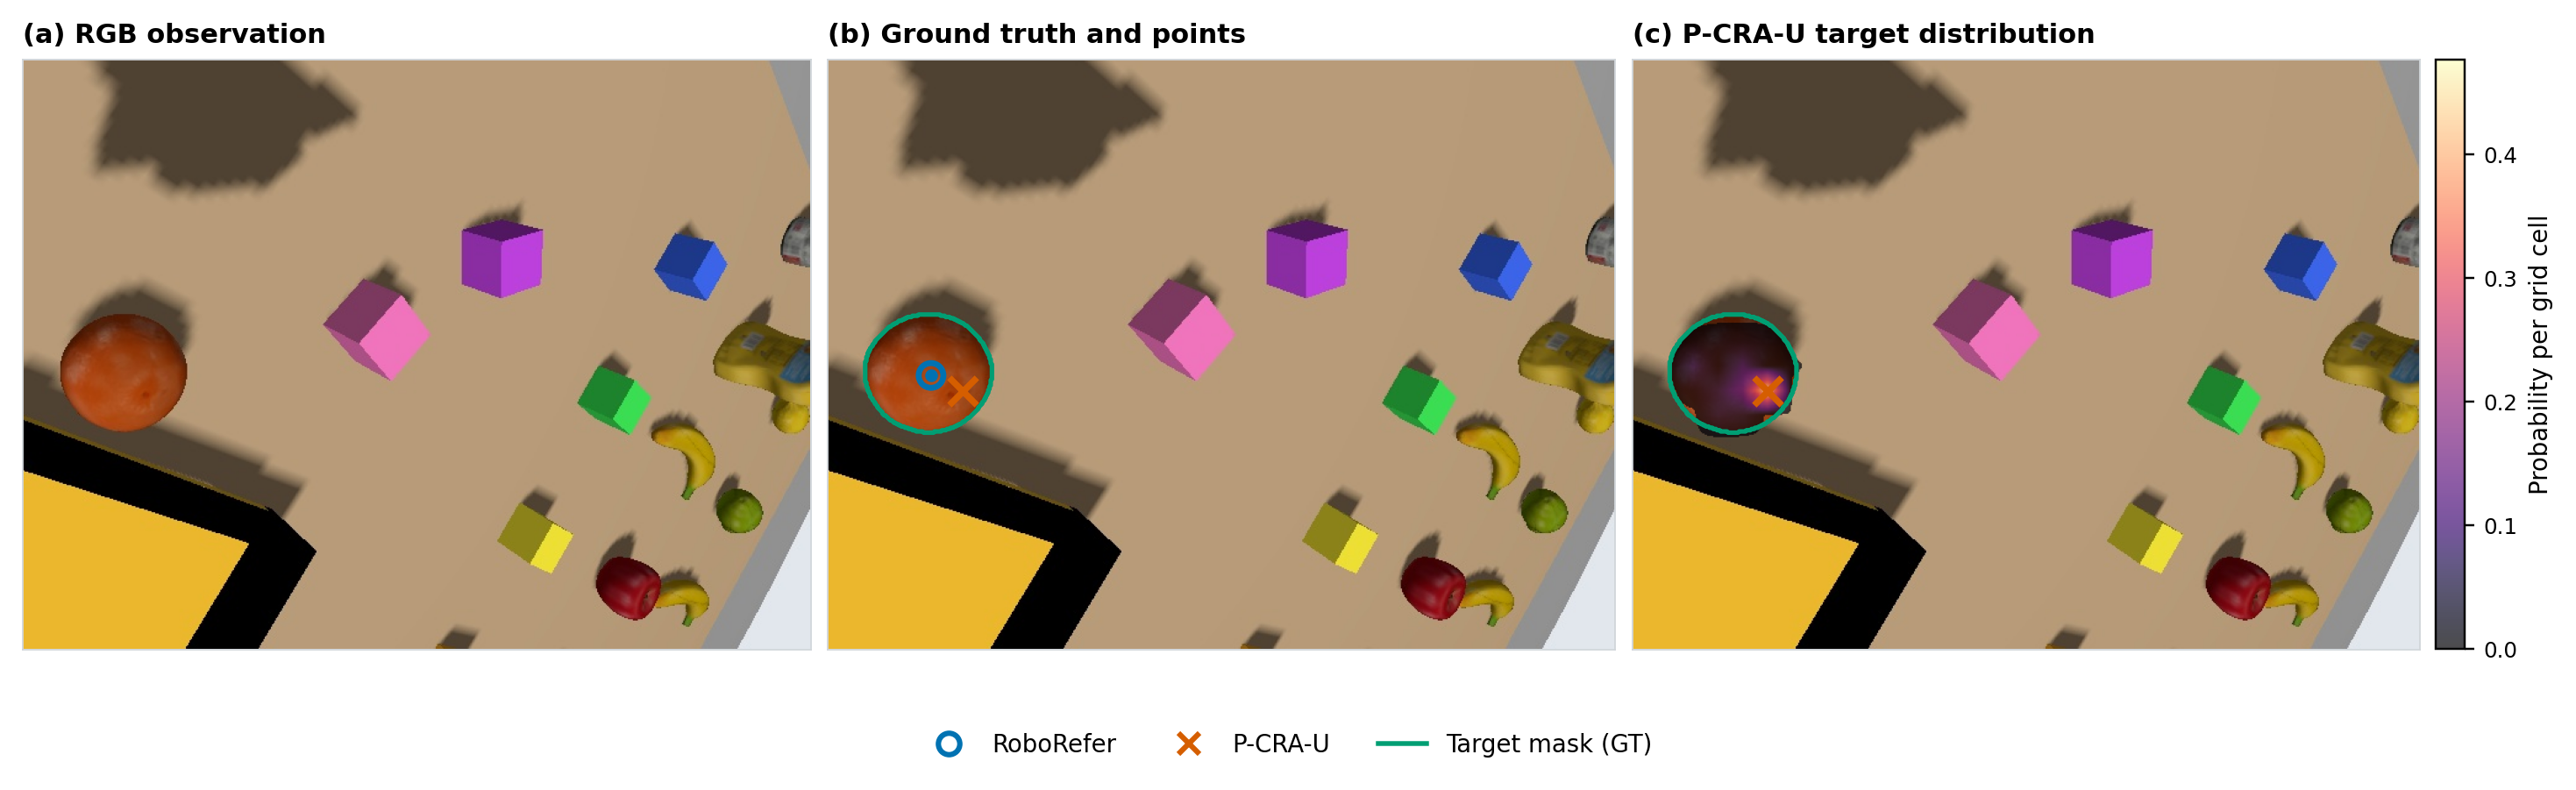
\includegraphics[width=\textwidth,height=0.65\textheight,keepaspectratio]{hinhanh/fig06_target_heatmap_real_rgb.png}
    \caption{Điểm RoboRefer, MAP và heatmap V2 trên RGB
    của sample \texttt{v211iid\_\allowbreak family\_\allowbreak 000127\_\allowbreak \_\allowbreak clean}.
    Heatmap nội suy để hiển thị từ lưới $24\times32$;
    ground-truth chỉ dùng đối chiếu sau suy luận.}
    \label{fig:results-target-heatmap}
    {\footnotesize Nguồn: capture Gazebo, prediction và
    evaluator Test-IID đã lưu; không phải ảnh robot vật lý.\par}
\end{figure}

Hình~\ref{fig:results-demo-spatial-distribution} cho thấy một
trường hợp mơ hồ khác: hai vùng xác suất nổi bật nằm gần hai ứng
viên của truy vấn. Điểm MAP là một lựa chọn theo phân bố vị trí,
chưa đủ để kết luận câu lệnh đã xác định được duy nhất một vật.

\begin{figure}[htbp]
    \centering
    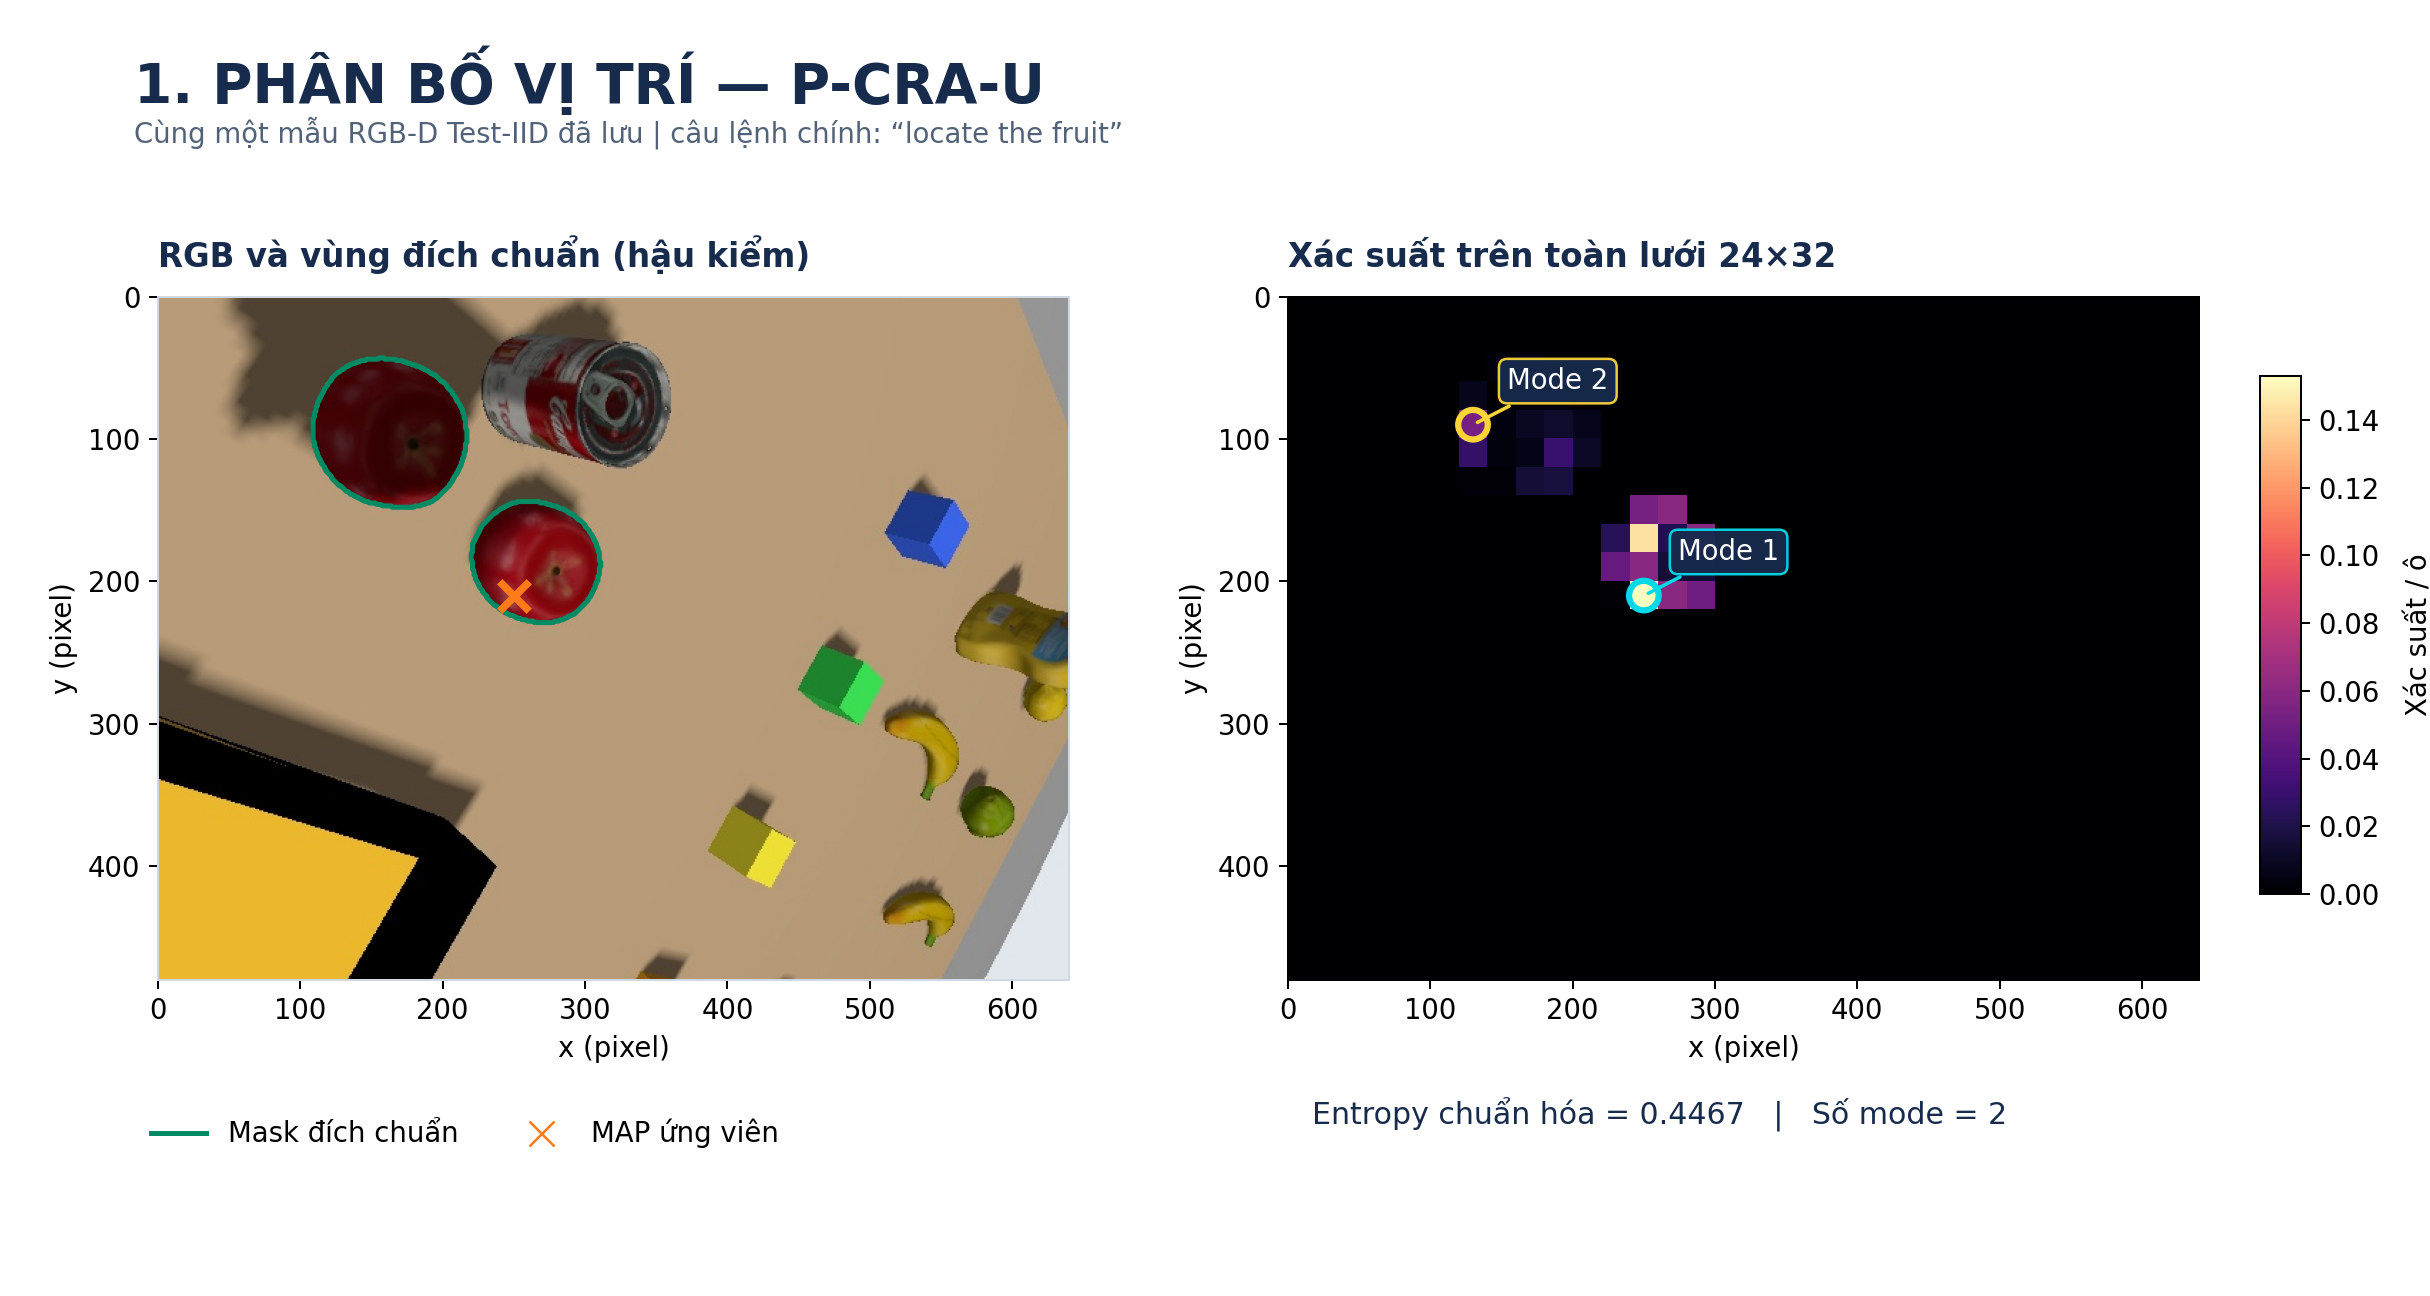
\includegraphics[width=\textwidth,height=0.66\textheight,keepaspectratio]{hinhanh/01_phan_bo_vi_tri.png}
    \caption{Minh họa phân bố vị trí của P-CRA-U trên sample
    \texttt{v211iid\_\allowbreak family\_\allowbreak 000137\_\allowbreak \_\allowbreak clean}. Hai mode là hai
    vùng ứng viên trên lưới $24\times32$; mask đích chuẩn chỉ
    được dùng để đối chiếu sau suy luận. Số mode không phải số
    instance đã nhận dạng.}
    \label{fig:results-demo-spatial-distribution}
\end{figure}

Target instance accuracy và top-$k$ instance recall
chưa có bảng đánh giá khóa đầy đủ. Một vật có thể tạo
nhiều đỉnh, hai vật có thể nằm trong một thành phần
xác suất; không suy ra các metric instance từ mode
count hay một heatmap minh họa.

\section{Đánh giá biểu diễn quan hệ}
\label{sec:results-relation}

\subsection{Kết quả edge head và giới hạn nhãn}

Accuracy trên cạnh hoạt động là $505/650=77.69\%$.
Mẫu số 650 là số cạnh đủ điều kiện theo evaluator,
không phải số câu lệnh. Nhãn edge là proxy supervision
của V2; metric không tương đương kiểm chứng độc lập
từng mệnh đề bằng hình học RGB-D.

\begin{table}[htbp]
    \centering
    \setlength{\tabcolsep}{4pt}
    \renewcommand{\arraystretch}{1.15}
    \caption{Bằng chứng hiện có cho relation/graph V2.}
    \label{tab:results-graph-evidence}
    \small
    \begin{tabularx}{\textwidth}{@{}>{\raggedright\arraybackslash}p{0.34\textwidth}r>{\raggedright\arraybackslash}X@{}}
        \toprule
        Chỉ số & Kết quả & Phạm vi \\
        \midrule
        Active-edge accuracy & 77.69\% & 505/650 cạnh với nhãn proxy \\
        Target extraction accuracy & -- & Chưa có semantic evaluator riêng \\
        Anchor extraction/localization & -- & Chưa có metric anchor đầy đủ \\
        Relation semantic macro-F1 & -- & Không thay bằng edge accuracy \\
        Edge precision/recall/F1 đầy đủ & -- & Chưa có bảng graph khóa tương ứng \\
        Multi-anchor exact match & -- & Chưa đánh giá toàn graph \\
        Oracle graph gap & -- & Chưa chạy oracle upper bound \\
        \bottomrule
    \end{tabularx}
    \vspace{2pt}
    {\footnotesize\raggedright Nguồn: \texttt{full\_\allowbreak metrics.json} và
    quy tắc supervision trong code V2; -- là chưa đánh giá.\par}
\end{table}

Cần phân biệt parse cấu trúc câu lệnh, dự đoán
anchor/edge evidence và định vị điểm cuối cùng.
Grounding theo nhóm \texttt{left\_\allowbreak of} hoặc
\texttt{between\_\allowbreak in\_\allowbreak depth} không phải accuracy parser
hay graph exact match.

Chưa có ablation bỏ relation slots, bỏ anchor head
hoặc dùng oracle graph trong điều kiện tương đương.
Mức tăng grounding vì vậy chỉ được quy cho toàn hệ
thống, không riêng relation-aware representation.
Đánh giá graph bổ sung phải lưu output trước khi
mở nhãn và định nghĩa khớp node, edge, slot rỗng cùng
trường hợp nhiều anchor.

Hình~\ref{fig:results-anchor-edge-case} cho thấy một ca có một
relation slot và một anchor slot hoạt động. Lưới anchor không có
trong file prediction Test-IID gốc, nên được trích xuất bổ sung
từ đúng checkpoint best V2 và feature cache đã khóa; score cạnh
hoạt động cùng điểm MAP được đối chiếu với prediction gốc.

\begin{figure}[htbp]
    \centering
    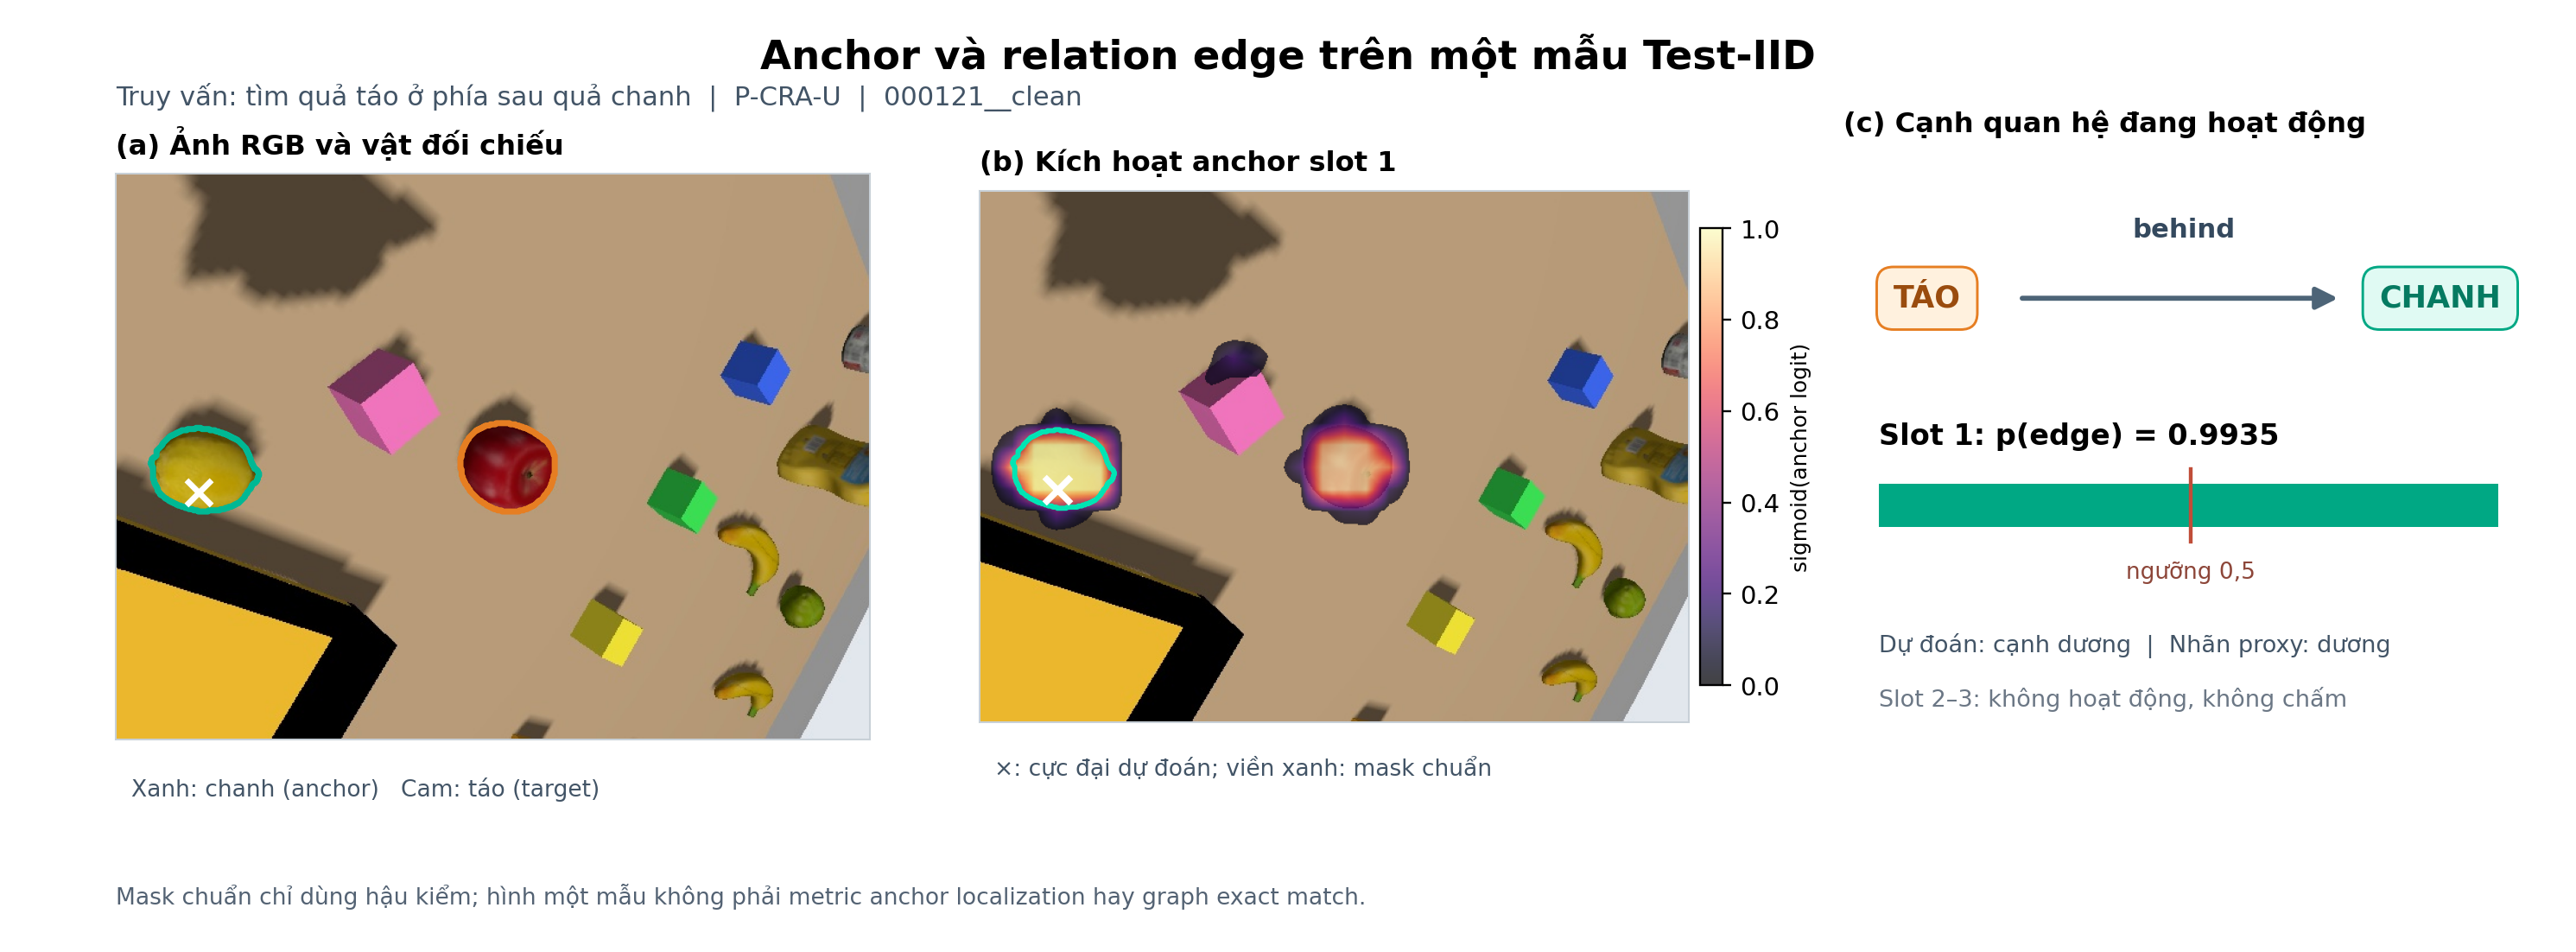
\includegraphics[width=\textwidth,height=0.62\textheight,keepaspectratio]{hinhanh/fig24_anchor_edge_test_iid.png}
    \caption{Anchor/edge evidence của P-CRA-U trên sample Test-IID
    \texttt{v211iid\_\allowbreak family\_\allowbreak 000121\_\allowbreak \_\allowbreak clean}: (a) RGB với mask
    target và anchor chỉ dùng hậu kiểm; (b) kích hoạt sigmoid của
    anchor slot 1 trên lưới $24\times32$, cực đại nằm trong mask
    quả chanh nhưng còn kích hoạt tại vùng quả táo; (c) cạnh
    \texttt{behind} đang hoạt động có score 0.9935, vượt ngưỡng 0.5
    và khớp nhãn proxy dương. Slot 2--3 không hoạt động, không
    được tính là cạnh dự đoán. Đây là ví dụ định tính, không phải
    metric anchor localization hay graph exact match.}
    \label{fig:results-anchor-edge-case}
    {\footnotesize Nguồn: RGB và mask evaluator-only Test-IID;
    checkpoint best V2 epoch 13/step 1120, feature cache và
    \texttt{predictions.jsonl} đã khóa.\par}
\end{figure}

\section{Đánh giá answerability}
\label{sec:results-answerability}

\subsection{Kết quả tổng thể và theo lớp}

Answerability được chấm trên toàn bộ 1000 sample.
Accuracy là 81.10\%, macro-F1 0.80969 và balanced accuracy 81.72\%.
So với V2 lịch sử, accuracy tăng 4.30 pp, macro-F1 tăng 0.03452.
CI 95\% paired theo family của chênh lệch macro-F1 là
$[0.01574,0.05392]$; CI của accuracy là $[2.30,6.40]$ pp.
Adapter sửa 71 ca phân loại sai nhưng làm sai thêm 28 ca, tăng ròng 43;
không phải mọi prediction đều cải thiện.

\begin{table}[htbp]
    \centering
    \setlength{\tabcolsep}{4pt}
    \renewcommand{\arraystretch}{1.15}
    \caption{Answerability của P-CRA-U có Adapter trên Test-IID.}
    \label{tab:results-answerability-class}
    \small
    \begin{tabularx}{\textwidth}{@{}>{\raggedright\arraybackslash}Xrrrr@{}}
        \toprule
        Lớp & Số mẫu & Precision & Recall & F1 \\
        \midrule
        FOUND & 420 & 0.8690 & 0.8690 & 0.8690 \\
        AMBIGUOUS & 105 & 1.0000 & 1.0000 & 1.0000 \\
        ABSENT & 132 & 0.5506 & 0.6591 & 0.6000 \\
        INSUFFICIENT & 343 & 0.8013 & 0.7405 & 0.7697 \\
        \bottomrule
    \end{tabularx}
    {\footnotesize\raggedright Nguồn: \texttt{answerability\_\allowbreak after} trong
    \texttt{test\_\allowbreak iid\_\allowbreak 7p5/full\_\allowbreak metrics.json}. INSUFFICIENT viết tắt
    INSUFFICIENT\_EVIDENCE. Precision/recall/F1 dùng thang $[0,1]$.\par}
\end{table}

Hình~\ref{fig:results-demo-answerability} đặt cạnh nhau bốn
trạng thái với xác suất dự đoán trên các sample Test-IID đã lưu.
Hình minh họa giữ xác suất V2 lịch sử; số liệu Adapter được báo ở bảng và ma trận mới. Trạng thái được xác định theo câu lệnh và bằng chứng quan sát;
chỉ nhìn thấy một vật trong ảnh không tự động có nghĩa là FOUND.

\begin{figure}[htbp]
    \centering
    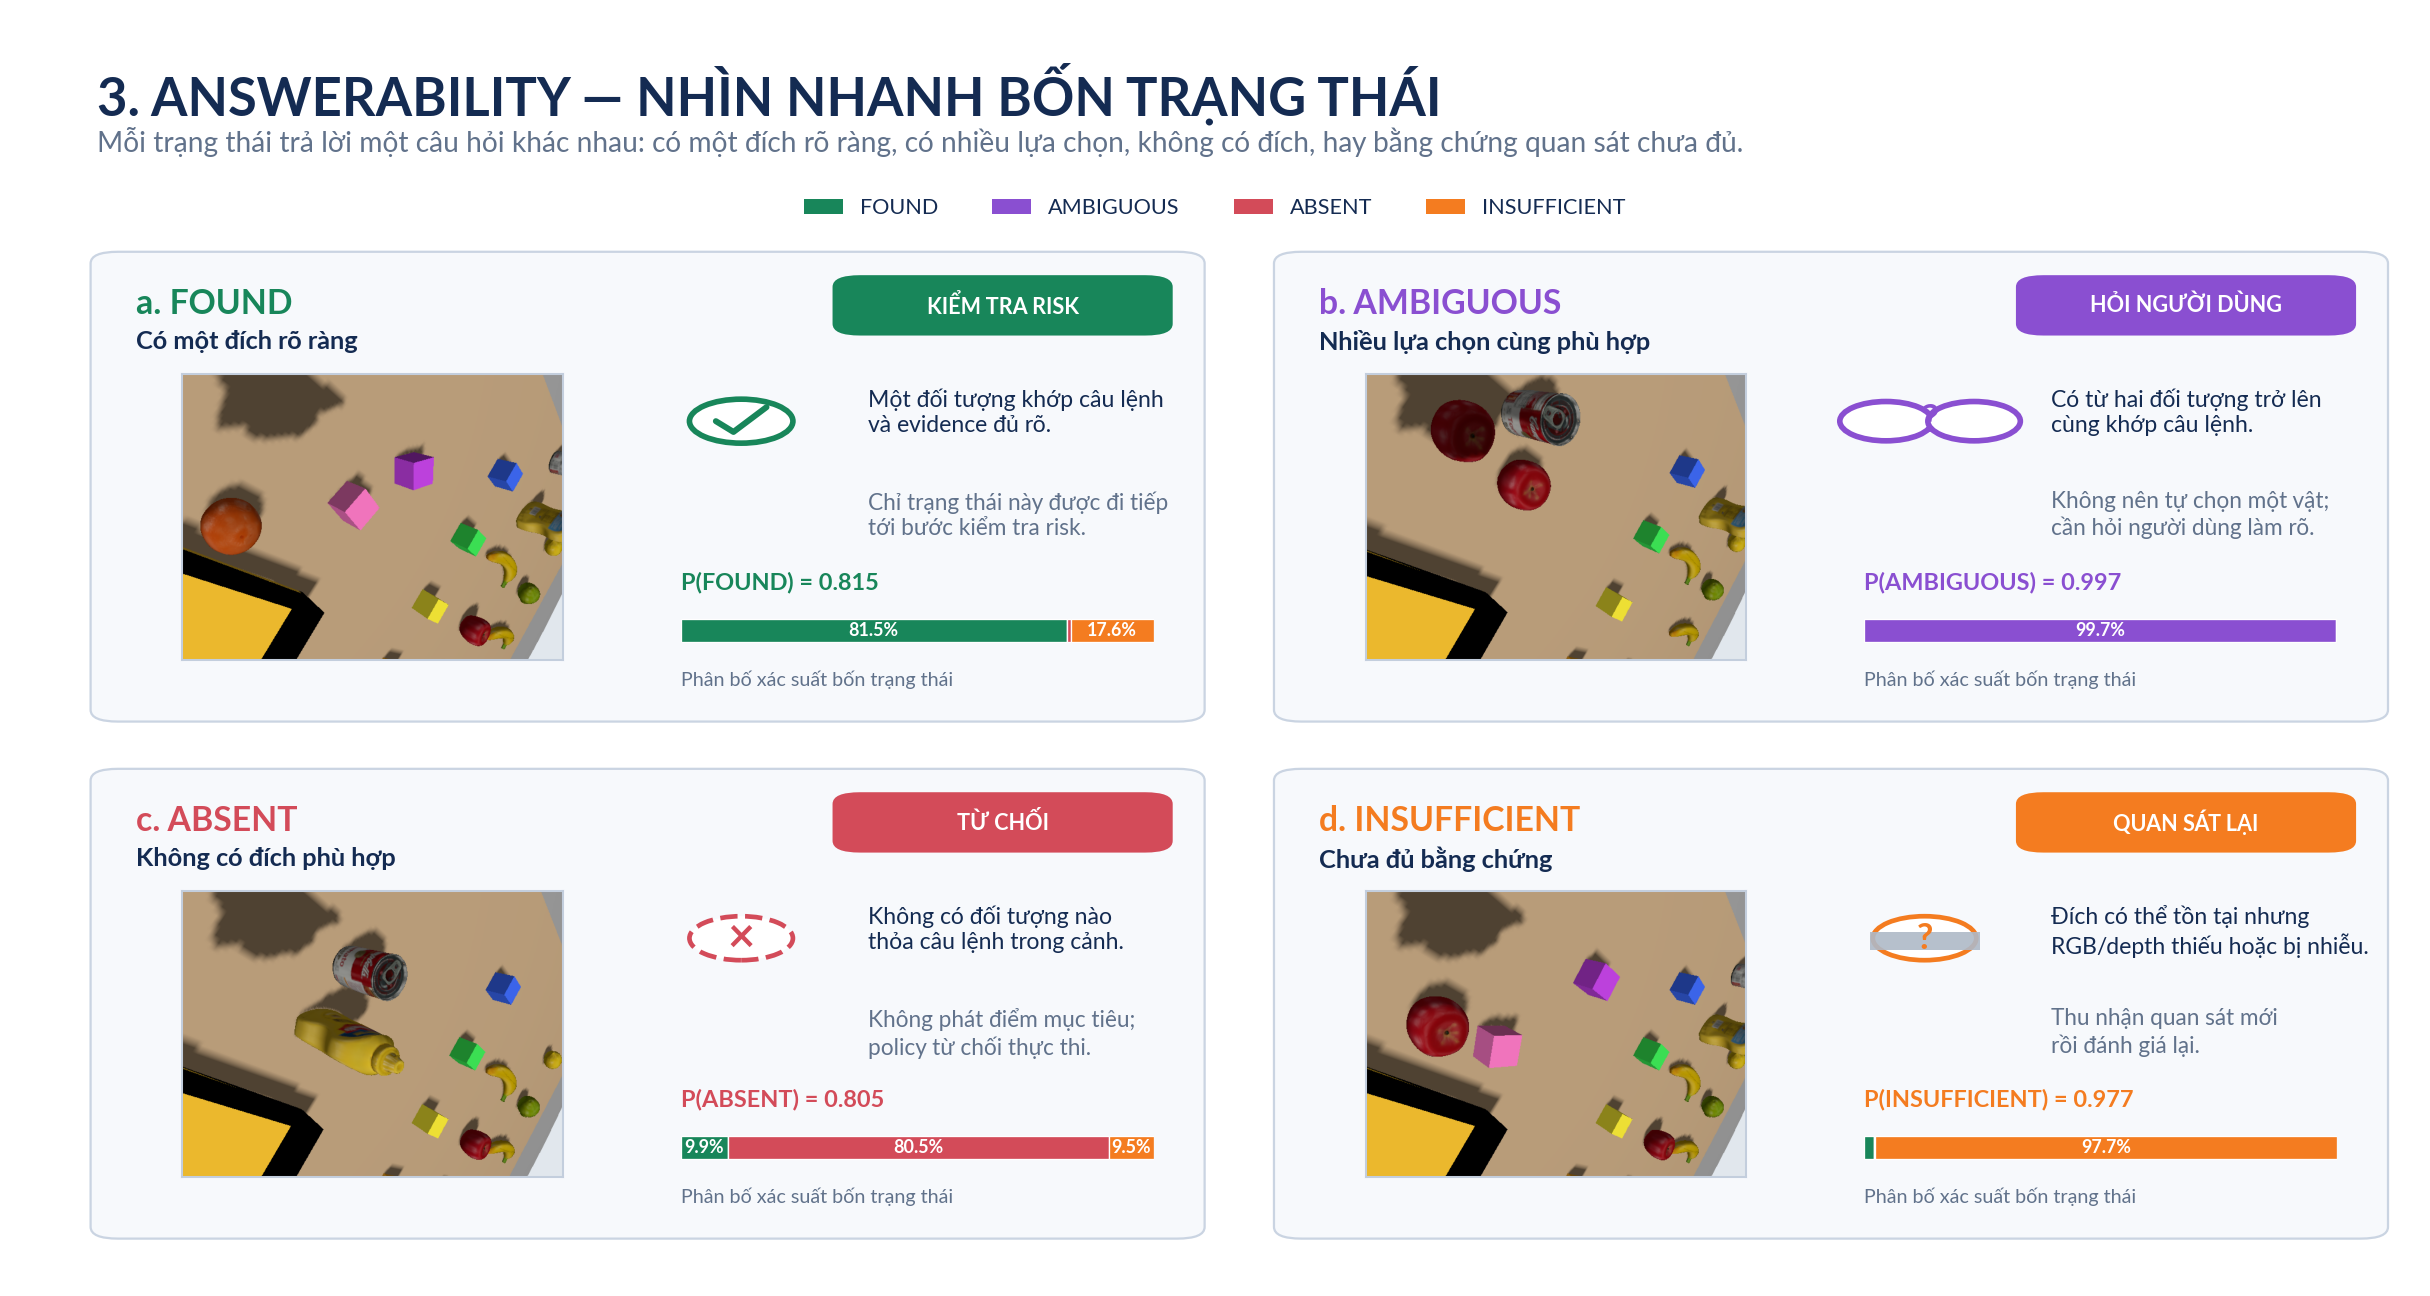
\includegraphics[width=\textwidth,height=0.68\textheight,keepaspectratio]{hinhanh/03_answerability.png}
    \caption{Bốn ví dụ answerability của V2 lịch sử: FOUND cho
    một đích rõ ràng, AMBIGUOUS cho nhiều lựa chọn, ABSENT cho
    truy vấn không có đích phù hợp và INSUFFICIENT\_EVIDENCE
    cho quan sát chưa đủ. Thanh màu thể hiện xác suất bốn lớp;
    thẻ FOUND minh họa bước kiểm tra risk trước khi policy
    có thể cho phép EXECUTE.}
    \label{fig:results-demo-answerability}
\end{figure}

\begin{table}[htbp]
    \centering
    \setlength{\tabcolsep}{4pt}
    \renewcommand{\arraystretch}{1.15}
    \caption{Confusion matrix answerability: hàng là nhãn thật,
    cột là dự đoán; đơn vị là số sample.}
    \label{tab:results-answerability-confusion}
    \small
    \begin{tabularx}{\textwidth}{@{}>{\raggedright\arraybackslash}Xrrrrr@{}}
        \toprule
        Nhãn thật & FOUND & AMBIG. & ABSENT & INSUFF. & Tổng \\
        \midrule
        FOUND & 365 & 0 & 22 & 33 & 420 \\
        AMBIGUOUS & 0 & 105 & 0 & 0 & 105 \\
        ABSENT & 15 & 0 & 87 & 30 & 132 \\
        INSUFFICIENT & 40 & 0 & 49 & 254 & 343 \\
        \midrule
        Tổng & 420 & 105 & 158 & 317 & 1000 \\
        \bottomrule

    \end{tabularx}
    \vspace{2pt}
    {\footnotesize\raggedright Nguồn: confusion matrix đã lưu.
    AMBIG.: AMBIGUOUS; INSUFF.: INSUFFICIENT\_EVIDENCE.\par}
\end{table}

AMBIGUOUS đạt 105/105 nhưng chỉ được xác nhận trong
registry và template hiện tại. Spatial source còn
dùng nhãn yếu suy từ AMBIGUOUS; không xem hai thành
tích này là hai bằng chứng độc lập về mọi dạng mơ hồ.

ABSENT vẫn yếu nhất, precision tăng từ 0.4913 lên 0.5506. Trong 158 dự đoán ABSENT có 71 mẫu thuộc lớp khác; 49 mẫu INSUFFICIENT\_EVIDENCE bị đoán ABSENT, giảm từ 57 của V2. Thiếu bằng chứng và không tồn tại vật
dẫn tới can thiệp khác nhau: quan sát lại có thể
phù hợp hơn từ chối khi vật vẫn hiện diện.

\subsection{False FOUND và ý nghĩa đối với policy}

\begin{table}[htbp]
    \centering
    \setlength{\tabcolsep}{4pt}
    \renewcommand{\arraystretch}{1.15}
    \caption{False FOUND trước cổng selective policy.}
    \label{tab:results-false-found}
    \small
    \begin{tabularx}{\textwidth}{@{}>{\raggedright\arraybackslash}Xrrr@{}}
        \toprule
        Nhãn thật & Dự đoán FOUND & Số mẫu & Tỉ lệ (\%) \\
        \midrule
        ABSENT & 15 & 132 & 11.36 \\
        AMBIGUOUS & 0 & 105 & 0.00 \\
        INSUFFICIENT & 40 & 343 & 11.66 \\
        \midrule
        Tất cả non-FOUND & 55 & 580 & 9.48 \\
        \bottomrule

    \end{tabularx}
    \vspace{2pt}
    {\footnotesize\raggedright Nguồn: confusion matrix answerability;
    đây chưa phải số lần EXECUTE hoặc robot thực thi sai.\par}
\end{table}

Trong 420 dự đoán FOUND có 55 false FOUND (13.10\%);
V2 có 70/415 (16.87\%). Đây khác False-FOUND 55/580 ở bảng tổng:
một tỉ lệ dùng mẫu số prediction FOUND, tỉ lệ kia dùng non-FOUND thật.
Policy mới vẫn chấp nhận 29 non-FOUND (7 ABSENT, 22 INSUFFICIENT),
nên giảm lỗi phân loại không tự bảo đảm giảm lỗi sau cổng vận hành.

Ở chiều ngược lại, 55/420 FOUND thật không được đoán FOUND:
22 ABSENT và 33 INSUFFICIENT, giảm từ 75/420 của V2.
Trên riêng 405 ca FOUND có MAP đúng, số bị cổng answerability chặn
giảm từ 66 xuống 48; Adapter sửa 30 nhưng làm sai thêm 12 ca hợp lệ.
Các con số 75 và 66 của V2 dùng hai mẫu số khác nhau, không hoán đổi.
Phân tích coverage cần thêm cổng risk, trình bày tại
Mục~\ref{sec:results-selective}.

\subsection{Chất lượng xác suất của head}

Multiclass Brier là 0.28002, NLL 0.51783 và confidence ECE 10 bin 0.07595; V2 lịch sử lần lượt là 0.32800, 0.57250 và 0.08566. Các giá trị mới tính từ xác suất Adapter đã lưu, không fit thêm bằng test. Đây là xác suất
bốn lớp answerability, khác với Brier/NLL/ECE
của risk nhị phân; không ghép hai nhóm như thể
cùng biến cố.

\begin{figure}[htbp]
    \centering
    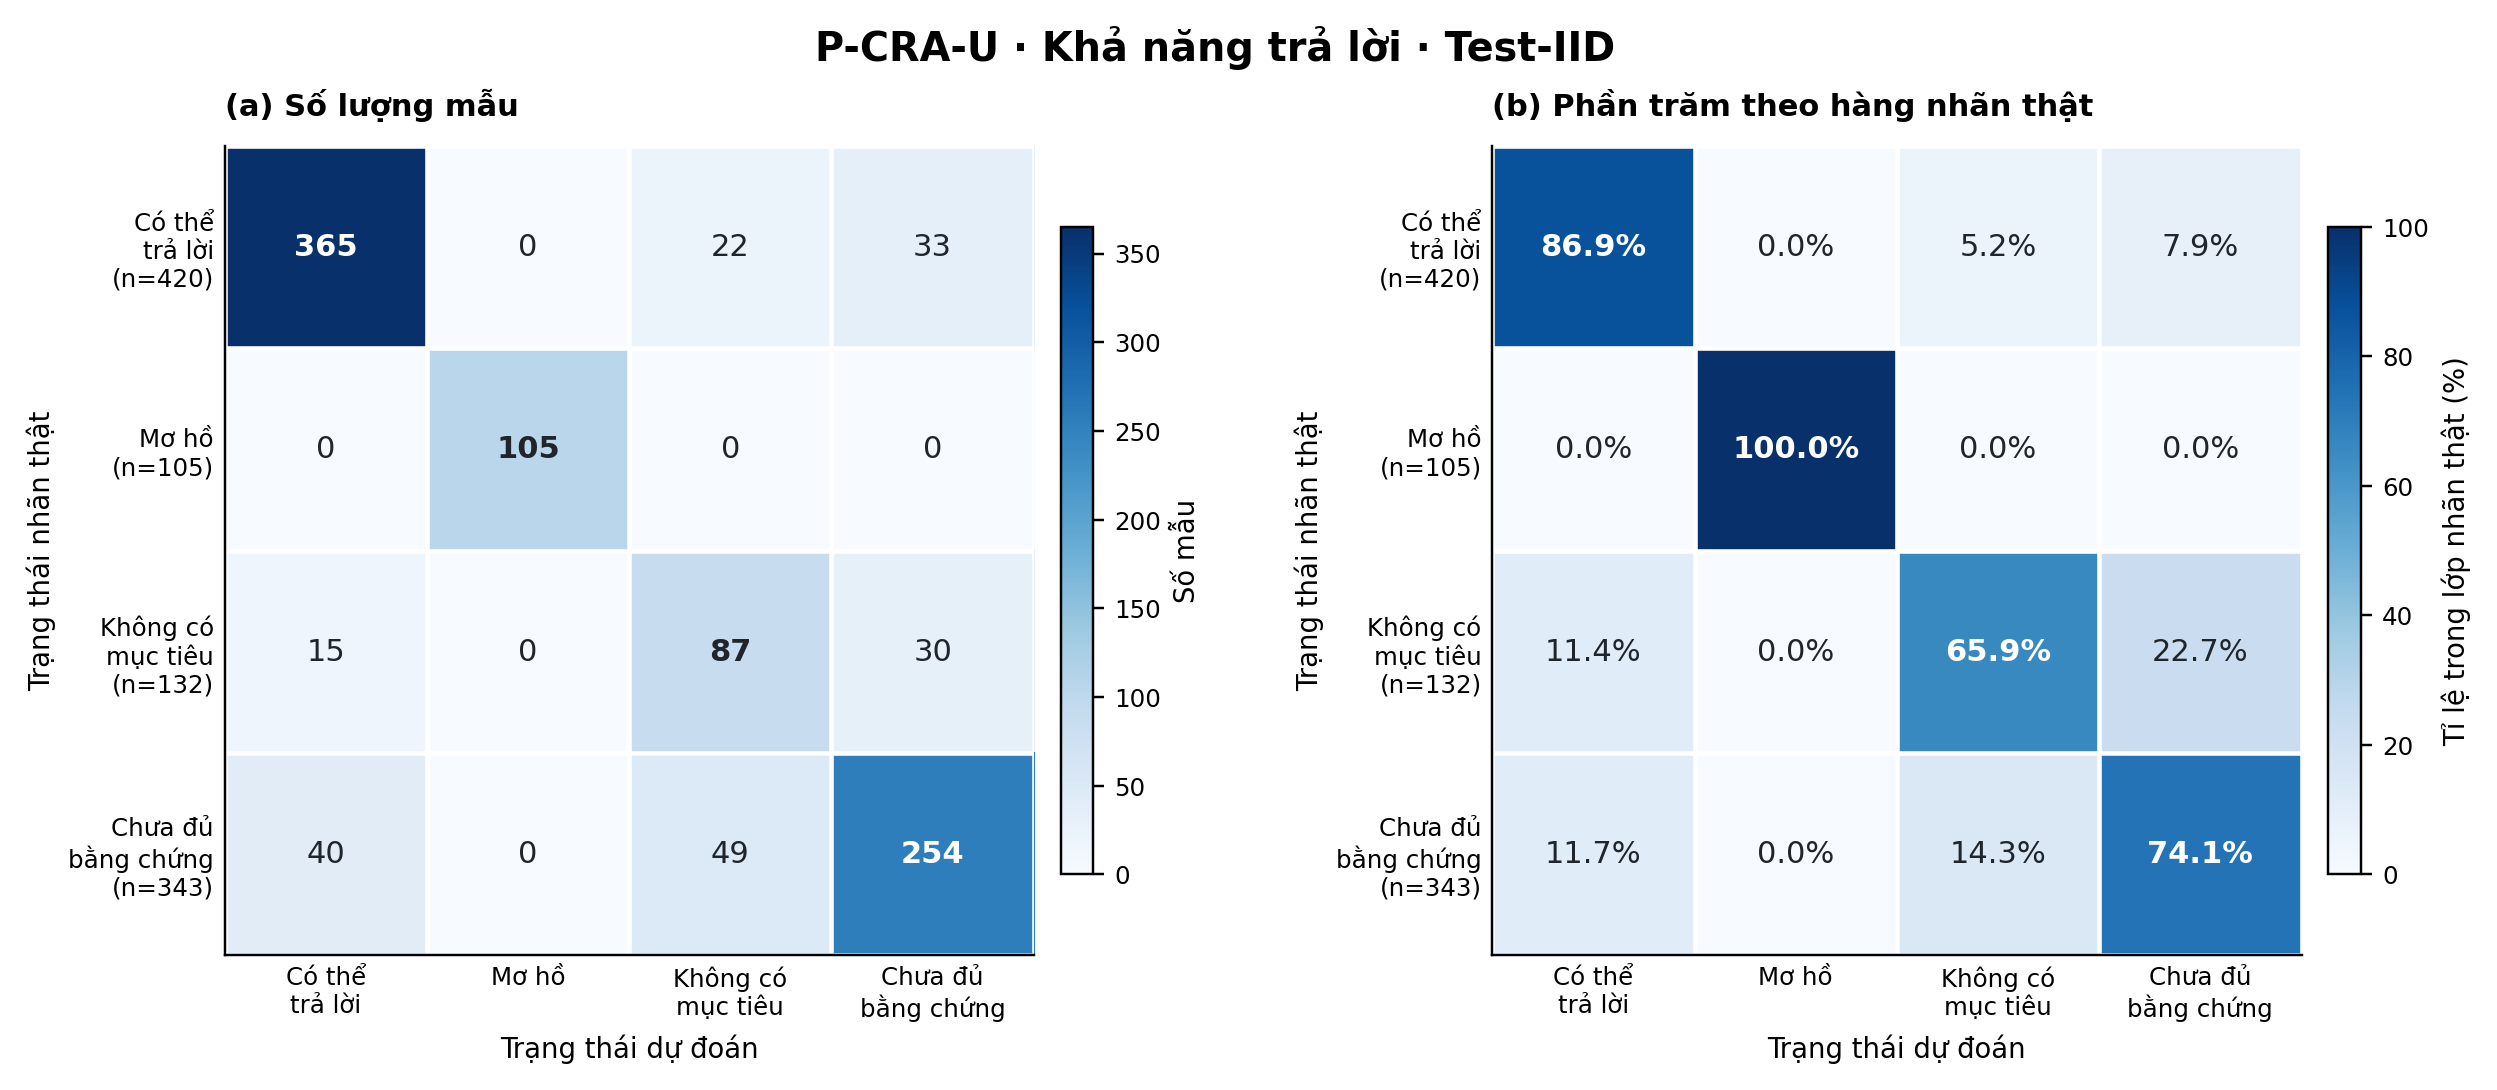
\includegraphics[width=\textwidth,height=0.60\textheight,keepaspectratio]{hinhanh/fig19_answerability_confusion_test_iid_adapter_vi.png}
    \caption{Confusion matrix answerability của P-CRA-U:
    (a) số sample; (b) tỉ lệ chuẩn hóa theo hàng nhãn thật.
    Hàng là ground-truth, cột là prediction; các ô đường
    chéo của (b) là recall từng lớp. Tổng cộng 1000 sample Test-IID.}
    \label{fig:results-answer-confusion-pending}
    {\footnotesize Nguồn: \texttt{answerability.confusion\_\allowbreak matrix}
    trong \texttt{full\_\allowbreak metrics.json}; dựng bằng Matplotlib
    từ kết quả đã khóa, không chạy lại suy luận.\par}
\end{figure}

\section{Khả năng phát hiện lỗi bằng uncertainty}
\label{sec:results-uncertainty}

\subsection{Biến cố lỗi và phạm vi kết luận}

Risk được chấm theo biến cố
\begin{equation}
    e_i=\mathbf{1}\left[
        y_i^{\mathrm{answer}}\neq\mathrm{FOUND}
        \;\lor\;
        \widehat{p}_i\notin M_i^{\mathrm{target}}
    \right].
    \label{eq:results-risk-event}
\end{equation}
Có 595 lỗi và 405 không lỗi trên 1000 sample.
580 lỗi đến từ non-FOUND, 15 lỗi còn lại là điểm
sai trên FOUND. Một AMBIGUOUS vẫn có thể hit mask
nhưng bị tính lỗi theo điều kiện chấp nhận câu
lệnh. AUROC risk không phải AUROC localization
failure đơn thuần.

\begin{table}[htbp]
    \centering
    \setlength{\tabcolsep}{4pt}
    \renewcommand{\arraystretch}{1.15}
    \caption{Phát hiện và xếp hạng biến cố lỗi của risk Adapter.}
    \label{tab:results-error-ranking}
    \small
    \begin{tabularx}{\textwidth}{@{}>{\raggedright\arraybackslash}Xr>{\raggedright\arraybackslash}X@{}}
        \toprule
        Chỉ số & Kết quả & Phạm vi \\
        \midrule
        Số lỗi / toàn bộ sample & 595/1000 &
        Biến cố ở Công thức~\eqref{eq:results-risk-event} \\
        AUROC $\uparrow$ & 0.95957 & Risk cao xếp lỗi lên trước \\
        Average precision (AP) $\uparrow$ & 0.96741 &
        Lớp dương là lỗi; prevalence 0.595 \\
        AURC $\downarrow$ & 0.25575 & Nhận dần theo risk tăng dần \\
        Oracle AURC & 0.22923 & Thứ tự oracle với cùng nhãn lỗi \\
        Excess-AURC $\downarrow$ & 0.02652 & AURC trừ oracle AURC \\
        \bottomrule
    \end{tabularx}
    \vspace{2pt}
    {\footnotesize\raggedright Nguồn: \texttt{risk\_\allowbreak calibration\_\allowbreak and\_\allowbreak ranking}
    trong \texttt{full\_\allowbreak metrics.json}. AP theo implementation
    đã lưu, không đổi thành cách tích phân PR khác.\par}
\end{table}

AUROC và AP cho thấy khả năng phân biệt tốt biến cố
tổng hợp. Tuy nhiên, non-FOUND chiếm phần lớn lỗi.
Chưa có bảng riêng về ranking 15 localization
failure trong FOUND; không suy ra mọi điểm sai
đều được phát hiện tốt như nhau từ AUROC tổng.

\subsection{Spatial distribution và bằng chứng mơ hồ}

Hình~\ref{fig:results-multimodal} minh họa một
sample mơ hồ có nhiều vùng xác suất. MAP đơn lẻ
không mô tả đầy đủ trạng thái này. Các vòng đánh
dấu đỉnh là cực đại cục bộ phục vụ trực quan,
không phải metric instance. Mode count của hậu
xử lý phụ thuộc ngưỡng và connected component.

\begin{figure}[htbp]
    \centering
    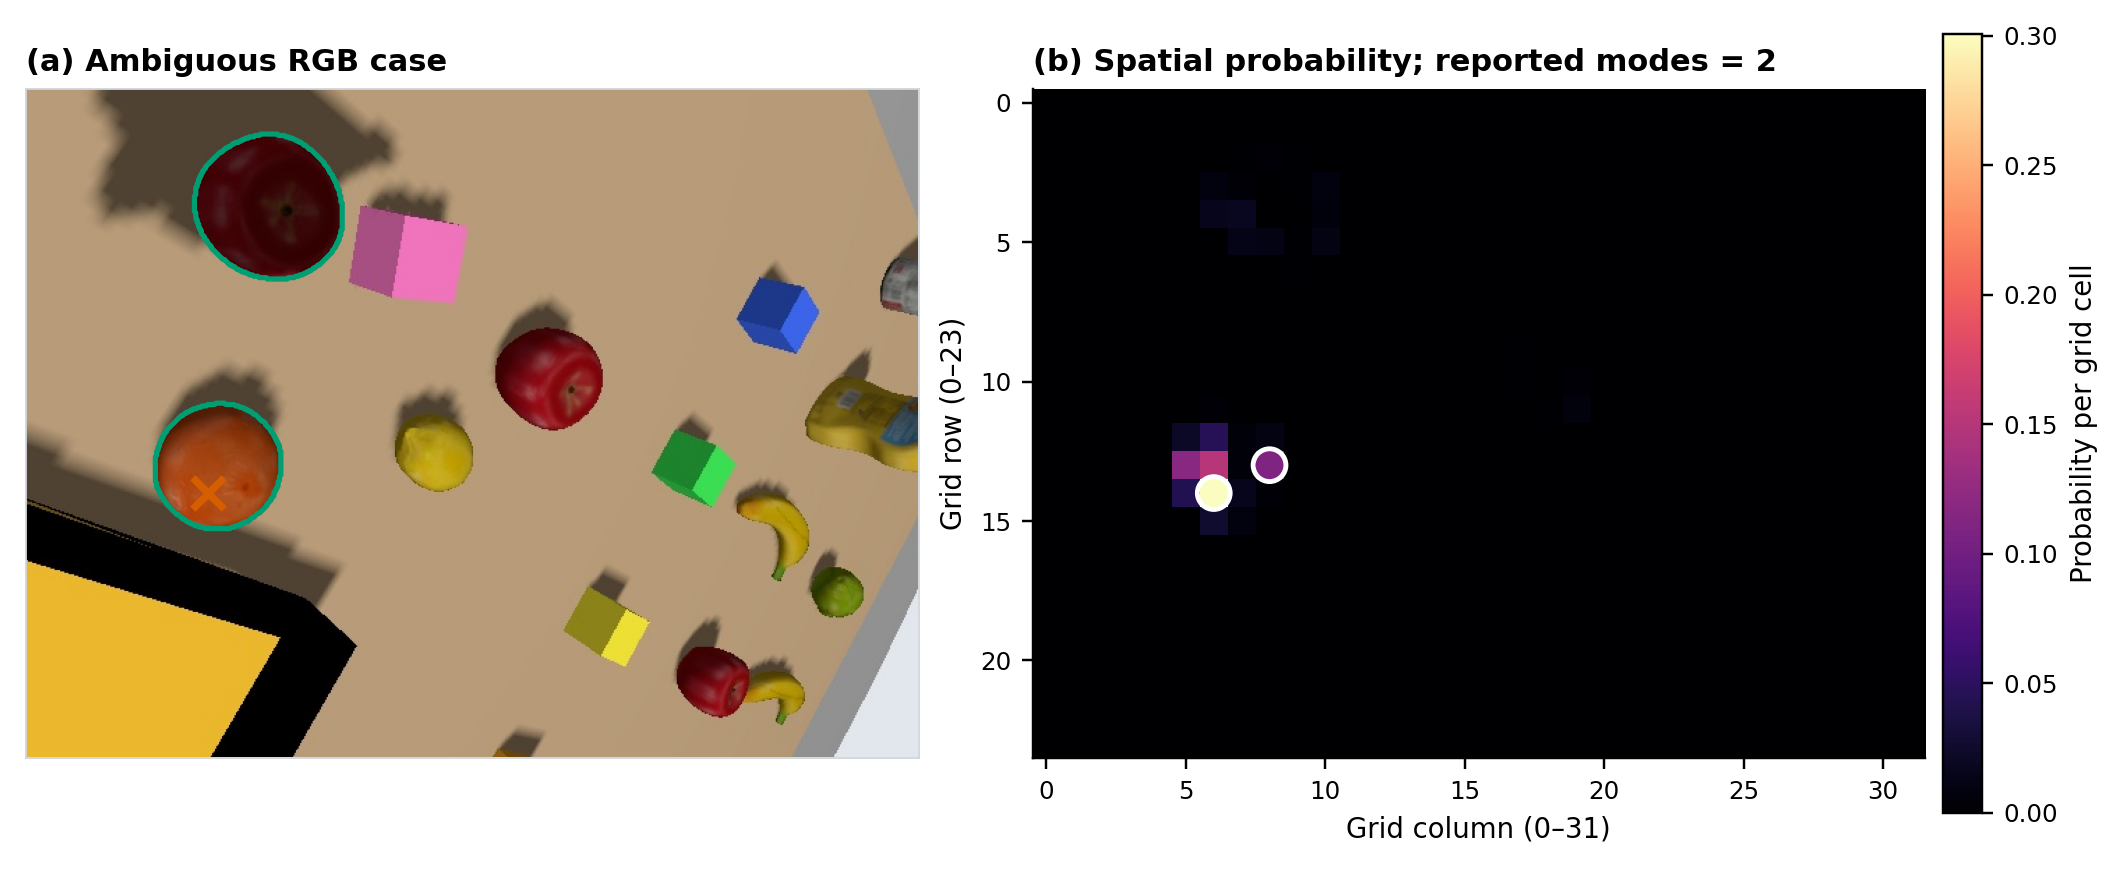
\includegraphics[width=\textwidth,height=0.65\textheight,keepaspectratio]{hinhanh/fig07_multimodal_spatial_distribution.png}
    \caption{Phân bố không gian đa đỉnh trên sample
    \texttt{v211iid\_\allowbreak family\_\allowbreak 000031\_\allowbreak \_\allowbreak clean}, nhãn AMBIGUOUS.
    Số vòng đánh dấu không được coi là số instance
    đã nhận dạng đúng.}
    \label{fig:results-multimodal}
    {\footnotesize Nguồn: RGB Gazebo, spatial prediction
    và evaluator Test-IID; GT chỉ dùng hậu kiểm.\par}
\end{figure}

Để tách localization failure khỏi trạng thái non-FOUND,
phân tích tương quan chỉ sử dụng 420 sample có nhãn thật
FOUND. Khoảng cách từ MAP tới target mask được ghép theo
sample ID từ kết quả paired; 405 sample có khoảng cách
bằng 0 và 15 sample có khoảng cách dương. Không loại
outlier, không thêm jitter và không chỉ lấy các điểm sai.

Hình~\ref{fig:results-localization-correlation-pending}
đối chiếu khoảng cách với entropy không gian chuẩn hóa,
$1-\text{peak margin}$ và calibrated risk. Phép biến đổi
$1-\text{peak margin}$ giúp cả ba trục có chiều tăng
hướng tới bất định/risk cao hơn. Pearson được tính trên
khoảng cách pixel gốc; Spearman dùng thứ hạng trung bình
cho các giá trị bằng nhau, bao gồm 405 khoảng cách bằng 0.
Thang symlog của trục khoảng cách chỉ phục vụ hiển thị,
không thay đổi dữ liệu dùng tính tương quan.

Entropy có Pearson $r=0.0148$ và Spearman
$\rho=0.0117$; $1-\text{peak margin}$ có $r=0.0146$
và $\rho=-0.0111$. Hai evidence không gian riêng lẻ
gần như không có liên hệ đơn điệu với khoảng cách
trên tập FOUND này. Calibrated risk Adapter có $r=0.2653$
và $\rho=0.1885$, thể hiện liên hệ dương nhưng còn yếu.
Risk được fit cho biến cố lỗi tổng hợp, không riêng
khoảng cách localization. Các hệ số là thống kê mô tả,
chưa có CI theo family hoặc kiểm định ý nghĩa;
không suy ra khả năng phát hiện mọi điểm sai.

\begin{figure}[htbp]
    \centering
    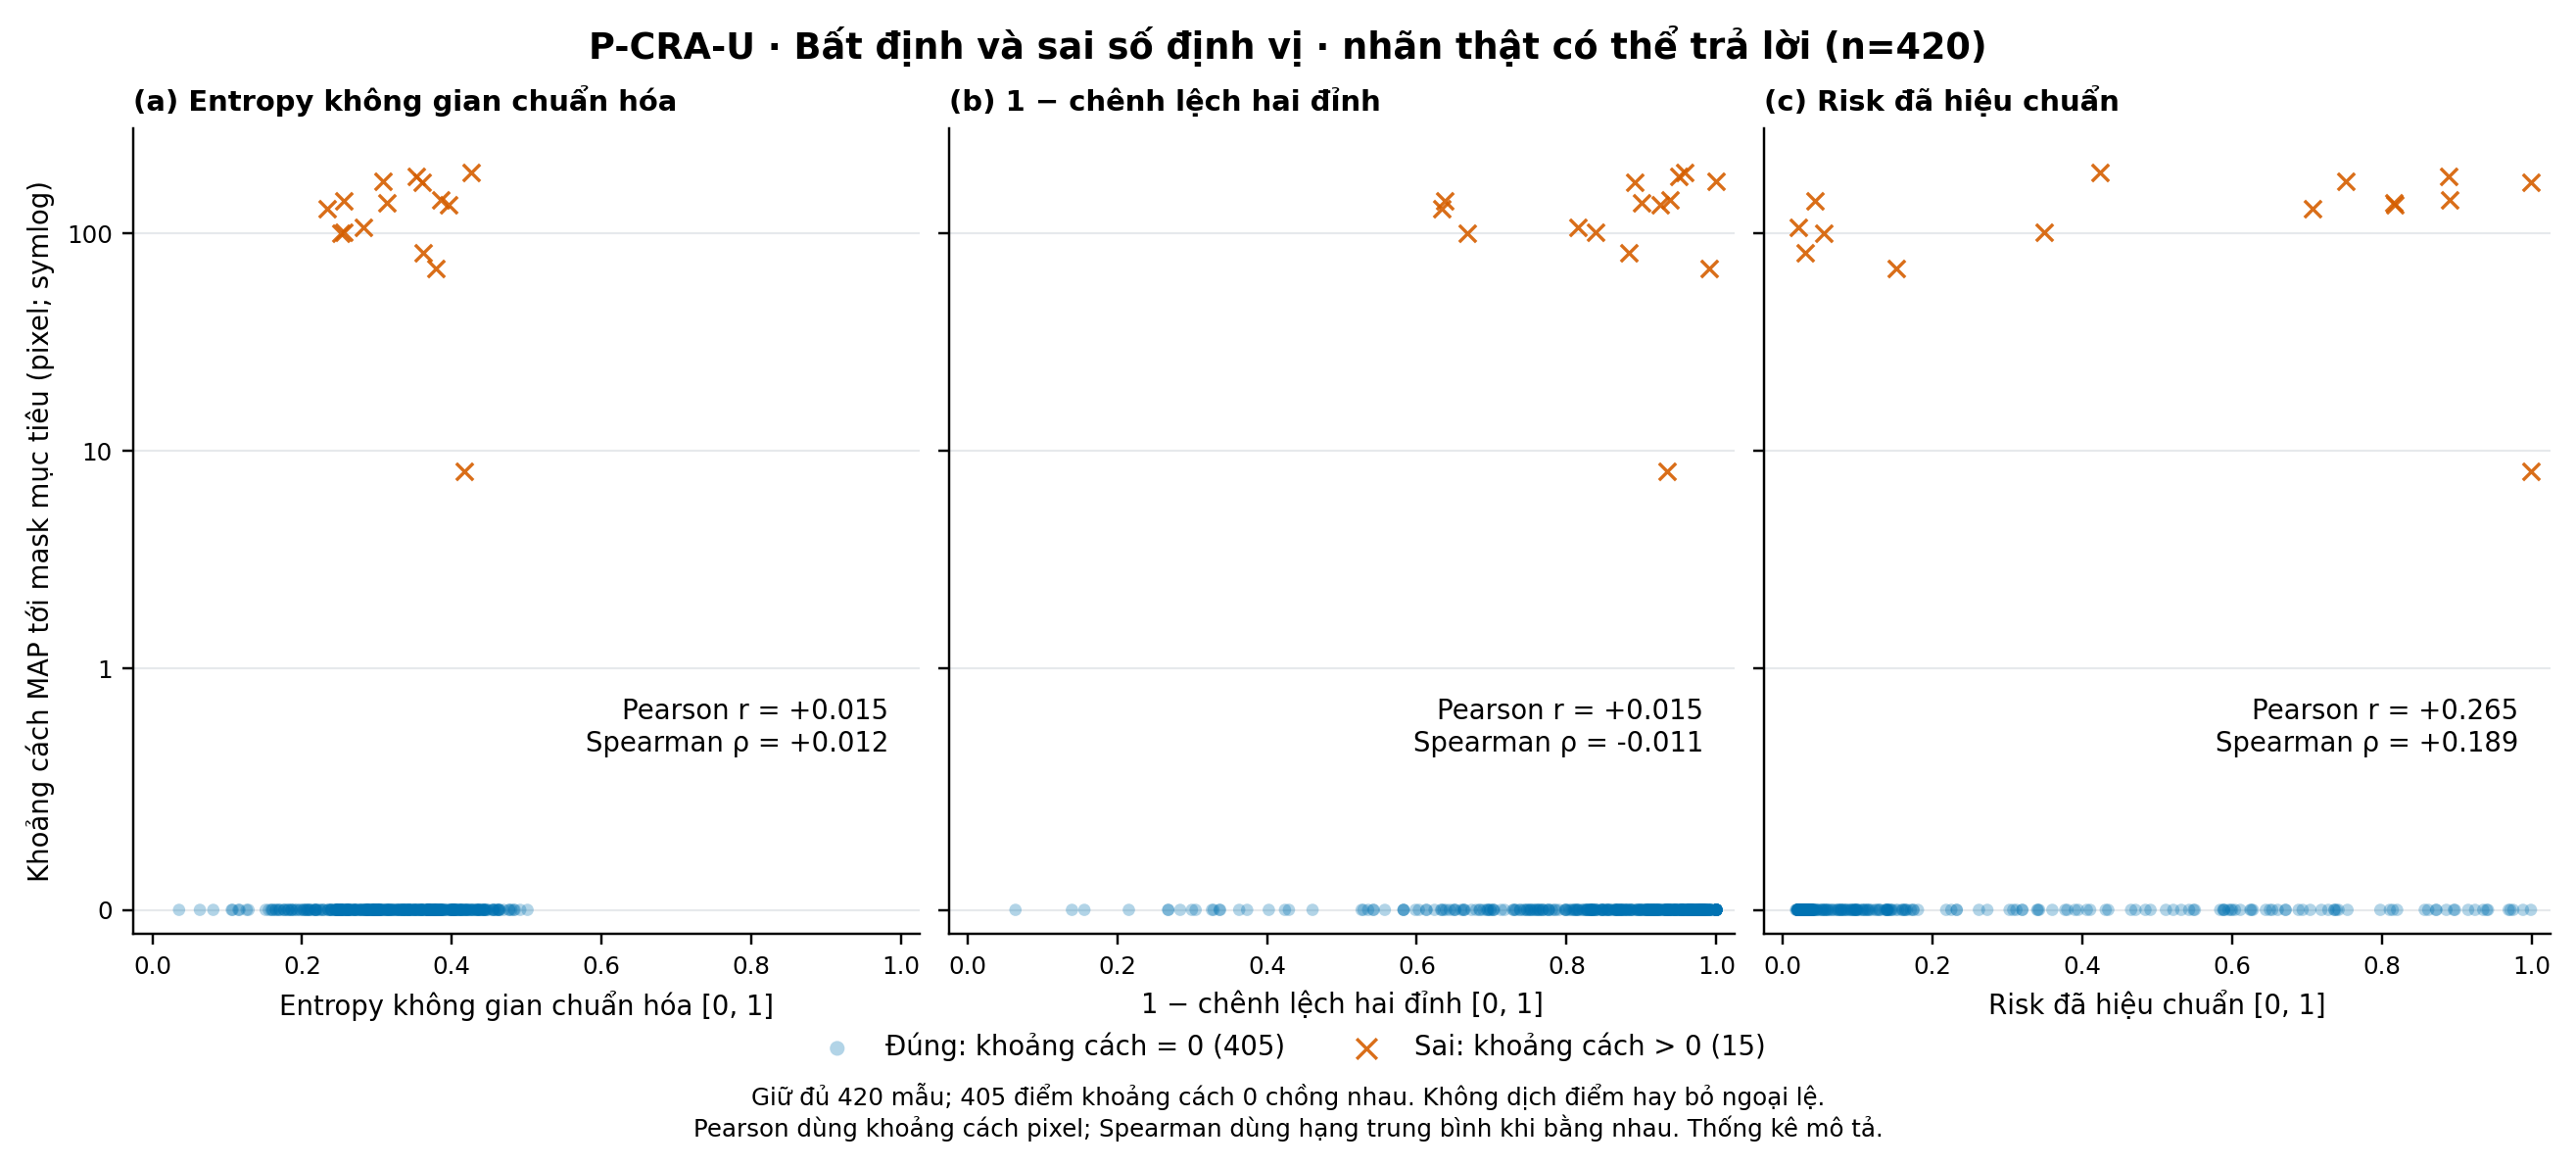
\includegraphics[width=\textwidth,height=0.58\textheight,keepaspectratio]{hinhanh/fig22_pcrau_uncertainty_localization_adapter_vi.png}
    \caption{Uncertainty--localization error của P-CRA-U
    trên 420 sample FOUND: (a) entropy chuẩn hóa;
    (b) $1-\text{peak margin}$; (c) calibrated risk.
    Khoảng cách tới mask có đơn vị pixel; trục tung dùng
    symlog để giữ cả giá trị 0. Các điểm đúng chồng nhau
    ở khoảng cách 0; không loại mẫu hoặc thêm jitter.
    Pearson dùng khoảng cách gốc, Spearman xử lý ties
    bằng thứ hạng trung bình.}
    \label{fig:results-localization-correlation-pending}
    {\footnotesize Nguồn: spatial evidence trong
    \texttt{predictions.jsonl}, risk trong
    \texttt{decisions.jsonl} và khoảng cách
    \texttt{v2\_\allowbreak distance\_\allowbreak px} trong \texttt{paired\_\allowbreak samples.csv};
    dựng bằng Matplotlib, không fit lại risk bằng test.\par}
\end{figure}

\section{Đánh giá source uncertainty}
\label{sec:results-source}

\subsection{Kết quả đa nhãn và từng source}

Source head sử dụng sigmoid độc lập cho semantic,
relation, spatial, depth và occlusion. Một sample có
thể có nhiều source dương, nên tổng support không
cần bằng 1000. Ngưỡng nhị phân của artifact V2 giữ
0.5 cho mọi source; không tối ưu lại ngưỡng trên test.

Macro-F1 năm source là 0.67739, micro-F1 0.62140,
macro-AUROC 0.88378 và macro-AP 0.70645.
Nếu không tính spatial nhãn yếu, macro-F1 bốn
source còn 0.59792. Giá trị thứ hai giúp tránh
để thành tích gần hoàn hảo của spatial che khuất
chất lượng attribution ở các source còn lại.

\begin{table}[htbp]
    \centering
    \setlength{\tabcolsep}{4pt}
    \renewcommand{\arraystretch}{1.15}
    \caption{Source uncertainty trên 1000 sample,
    threshold 0.5. Các metric dùng thang $[0,1]$.}
    \label{tab:results-source-main}
    \small
    \begin{tabularx}{\textwidth}{@{}>{\raggedright\arraybackslash}Xrrrrrrr@{}}
        \toprule
        Nguồn & $n_+$ & \shortstack{Preci-\\sion} & Recall & F1 & \shortstack{Speci-\\ficity} & AUROC & AP \\
        \midrule
        Semantic & 237 & 0.3804 & 0.7046 & 0.4941 & 0.6435 & 0.7766 & 0.6028 \\
        Relation & 237 & 0.4987 & 0.8228 & 0.6210 & 0.7431 & 0.8650 & 0.6706 \\
        Spatial$^\dagger$ & 105 & 0.9906 & 1.0000 & 0.9953 & 0.9989 & 1.0000 & 1.0000 \\
        Depth & 160 & 0.6364 & 0.7875 & 0.7039 & 0.9143 & 0.9156 & 0.7132 \\
        Occlusion & 183 & 0.4797 & 0.7104 & 0.5727 & 0.8274 & 0.8617 & 0.5457 \\
        \midrule
        \multicolumn{4}{@{}l}{Macro, 5 nguồn} & 0.6774 & -- & 0.8838 & 0.7065 \\
        \multicolumn{4}{@{}l}{Micro-F1, 5 nguồn} & 0.6214 & -- & -- & -- \\
        \multicolumn{4}{@{}l}{Macro-F1, bỏ spatial} & 0.5979 & -- & -- & -- \\
        \bottomrule
    \end{tabularx}
    \vspace{2pt}
    {\footnotesize\raggedright Nguồn: \texttt{full\_\allowbreak metrics.json};
    macro bỏ spatial tính từ bốn F1 tương ứng.
    $^\dagger$Spatial dùng nhãn yếu suy từ AMBIGUOUS,
    không phải nguồn lỗi nhân quả được đo độc lập.\par}
\end{table}

\begin{table}[htbp]
    \centering
    \setlength{\tabcolsep}{4pt}
    \renewcommand{\arraystretch}{1.15}
    \caption{Phân rã lỗi và chất lượng xác suất từng source.}
    \label{tab:results-source-errors}
    \small
    \begin{tabularx}{\textwidth}{@{}>{\raggedright\arraybackslash}Xrrrrrrr@{}}
        \toprule
        Nguồn & TP & FP & FN & TN & \shortstack{Dự đoán\\dương} & Brier & ECE$_{10}$ \\
        \midrule
        Semantic & 167 & 272 & 70 & 491 & 439 & 0.18873 & 0.18930 \\
        Relation & 195 & 196 & 42 & 567 & 391 & 0.16444 & 0.19976 \\
        Spatial$^\dagger$ & 105 & 1 & 0 & 894 & 106 & 0.00177 & 0.01445 \\
        Depth & 126 & 72 & 34 & 768 & 198 & 0.08957 & 0.08794 \\
        Occlusion & 130 & 141 & 53 & 676 & 271 & 0.13104 & 0.11258 \\
        \bottomrule
    \end{tabularx}
    \vspace{2pt}
    {\footnotesize\raggedright Nguồn: thống kê per-source Test-IID.
    TP/FP/FN/TN của mỗi hàng cộng thành 1000;
    source Brier/ECE không phải risk Brier/ECE.\par}
\end{table}

Depth là source không yếu có F1 và AP cao nhất.
Semantic có 272 false positive, nhiều hơn 167
true positive; precision chỉ 0.3804. Occlusion
có 141 false positive so với 130 true positive.
Các score này hữu ích như evidence nhưng chưa
đủ tin cậy để coi mỗi cảnh báo là nguyên nhân
thực sự của một lỗi grounding.

Relation có recall 0.8228 nhưng specificity
0.7431, cho thấy thiên về phát hiện nhiều
trường hợp dương và chấp nhận cảnh báo thừa.
Nếu muốn giảm false positive bằng threshold
riêng, phải fit trên calibration trong một
experiment mới và đánh giá bằng protocol phù
hợp; không chỉnh V2 sau khi đã xem Test-IID.

\subsection{Phản ứng paired trước thay đổi bằng chứng}

Với mỗi family, so sánh source probability của
variant với clean:
\begin{equation}
    \Delta u_{f,s}^{(v)}
    =u_{f,s}^{(v)}-u_{f,s}^{(\mathrm{clean})}.
    \label{eq:results-source-delta}
\end{equation}
Mỗi loại variant có 200 cặp family. Bảng dưới
là trung bình chênh lệch xác suất, không phải
logit hay phần trăm accuracy. Đây là phân tích
mô tả từ prediction có sẵn, không fit thêm mô hình.

\begin{table}[htbp]
    \centering
    \setlength{\tabcolsep}{4pt}
    \renewcommand{\arraystretch}{1.15}
    \caption{Thay đổi source probability so với clean,
    trung bình trên 200 cặp family cho mỗi variant.}
    \label{tab:results-source-delta}
    \small
    \begin{tabularx}{\textwidth}{@{}>{\raggedright\arraybackslash}Xrrrrrr@{}}
        \toprule
        Variant & $\Delta u_{\rm sem}$ & $\Delta u_{\rm rel}$ & $\Delta u_{\rm spat}$ & $\Delta u_{\rm dep}$ & $\Delta u_{\rm occ}$ & \shortstack{Nguồn tương\\ứng tăng} \\
        \midrule
        Semantic CF & $+0.2202$ & $-0.2089$ & $-0.1823$ & $-0.2214$ & $-0.3297$ & 162/200 \\
        Relation CF & $+0.0561$ & $+0.0723$ & $-0.1776$ & $-0.1192$ & $-0.1439$ & 130/200 \\
        Depth corruption & $+0.0950$ & $+0.0155$ & $+0.0079$ & $+0.4304$ & $-0.0890$ & 194/200 \\
        Occlusion/view CF & $-0.0398$ & $-0.0417$ & $-0.0025$ & $-0.0104$ & $+0.1860$ & 176/200 \\
        \bottomrule
    \end{tabularx}
    \vspace{2pt}
    {\footnotesize\raggedright Nguồn: source probability đã lưu, ghép
    clean--variant theo family. Cột cuối đếm $\Delta u>0$
    của source cùng tên variant. Chưa có CI cho bảng này.\par}
\end{table}

Depth tăng trung bình 0.4304 và tăng ở 194/200
cặp, trong khi semantic tăng 0.0950 và relation
chỉ tăng 0.0155. Đây là dấu hiệu phản ứng có
tính chọn lọc tương đối đối với perturbation
depth. Occlusion tăng 0.1860 ở trung bình và
tăng ở 176/200 cặp. Relation có thay đổi nhỏ
hơn, tăng trung bình 0.0723 ở 130/200 cặp.

Tuy nhiên, semantic CF không đồng nghĩa câu
lệnh vô nghiệm: variant có thể chọn một vật
khác và vẫn FOUND. Việc semantic probability
tăng chỉ chứng minh mô hình phản ứng với
thay đổi câu lệnh, không tự chứng minh nhãn
semantic uncertainty phải dương. Chính hiện
tượng này góp phần giải thích false positive.
Các thay đổi source là bằng chứng mô tả,
không xác lập attribution nhân quả độc lập.

\begin{figure}[htbp]
    \centering
    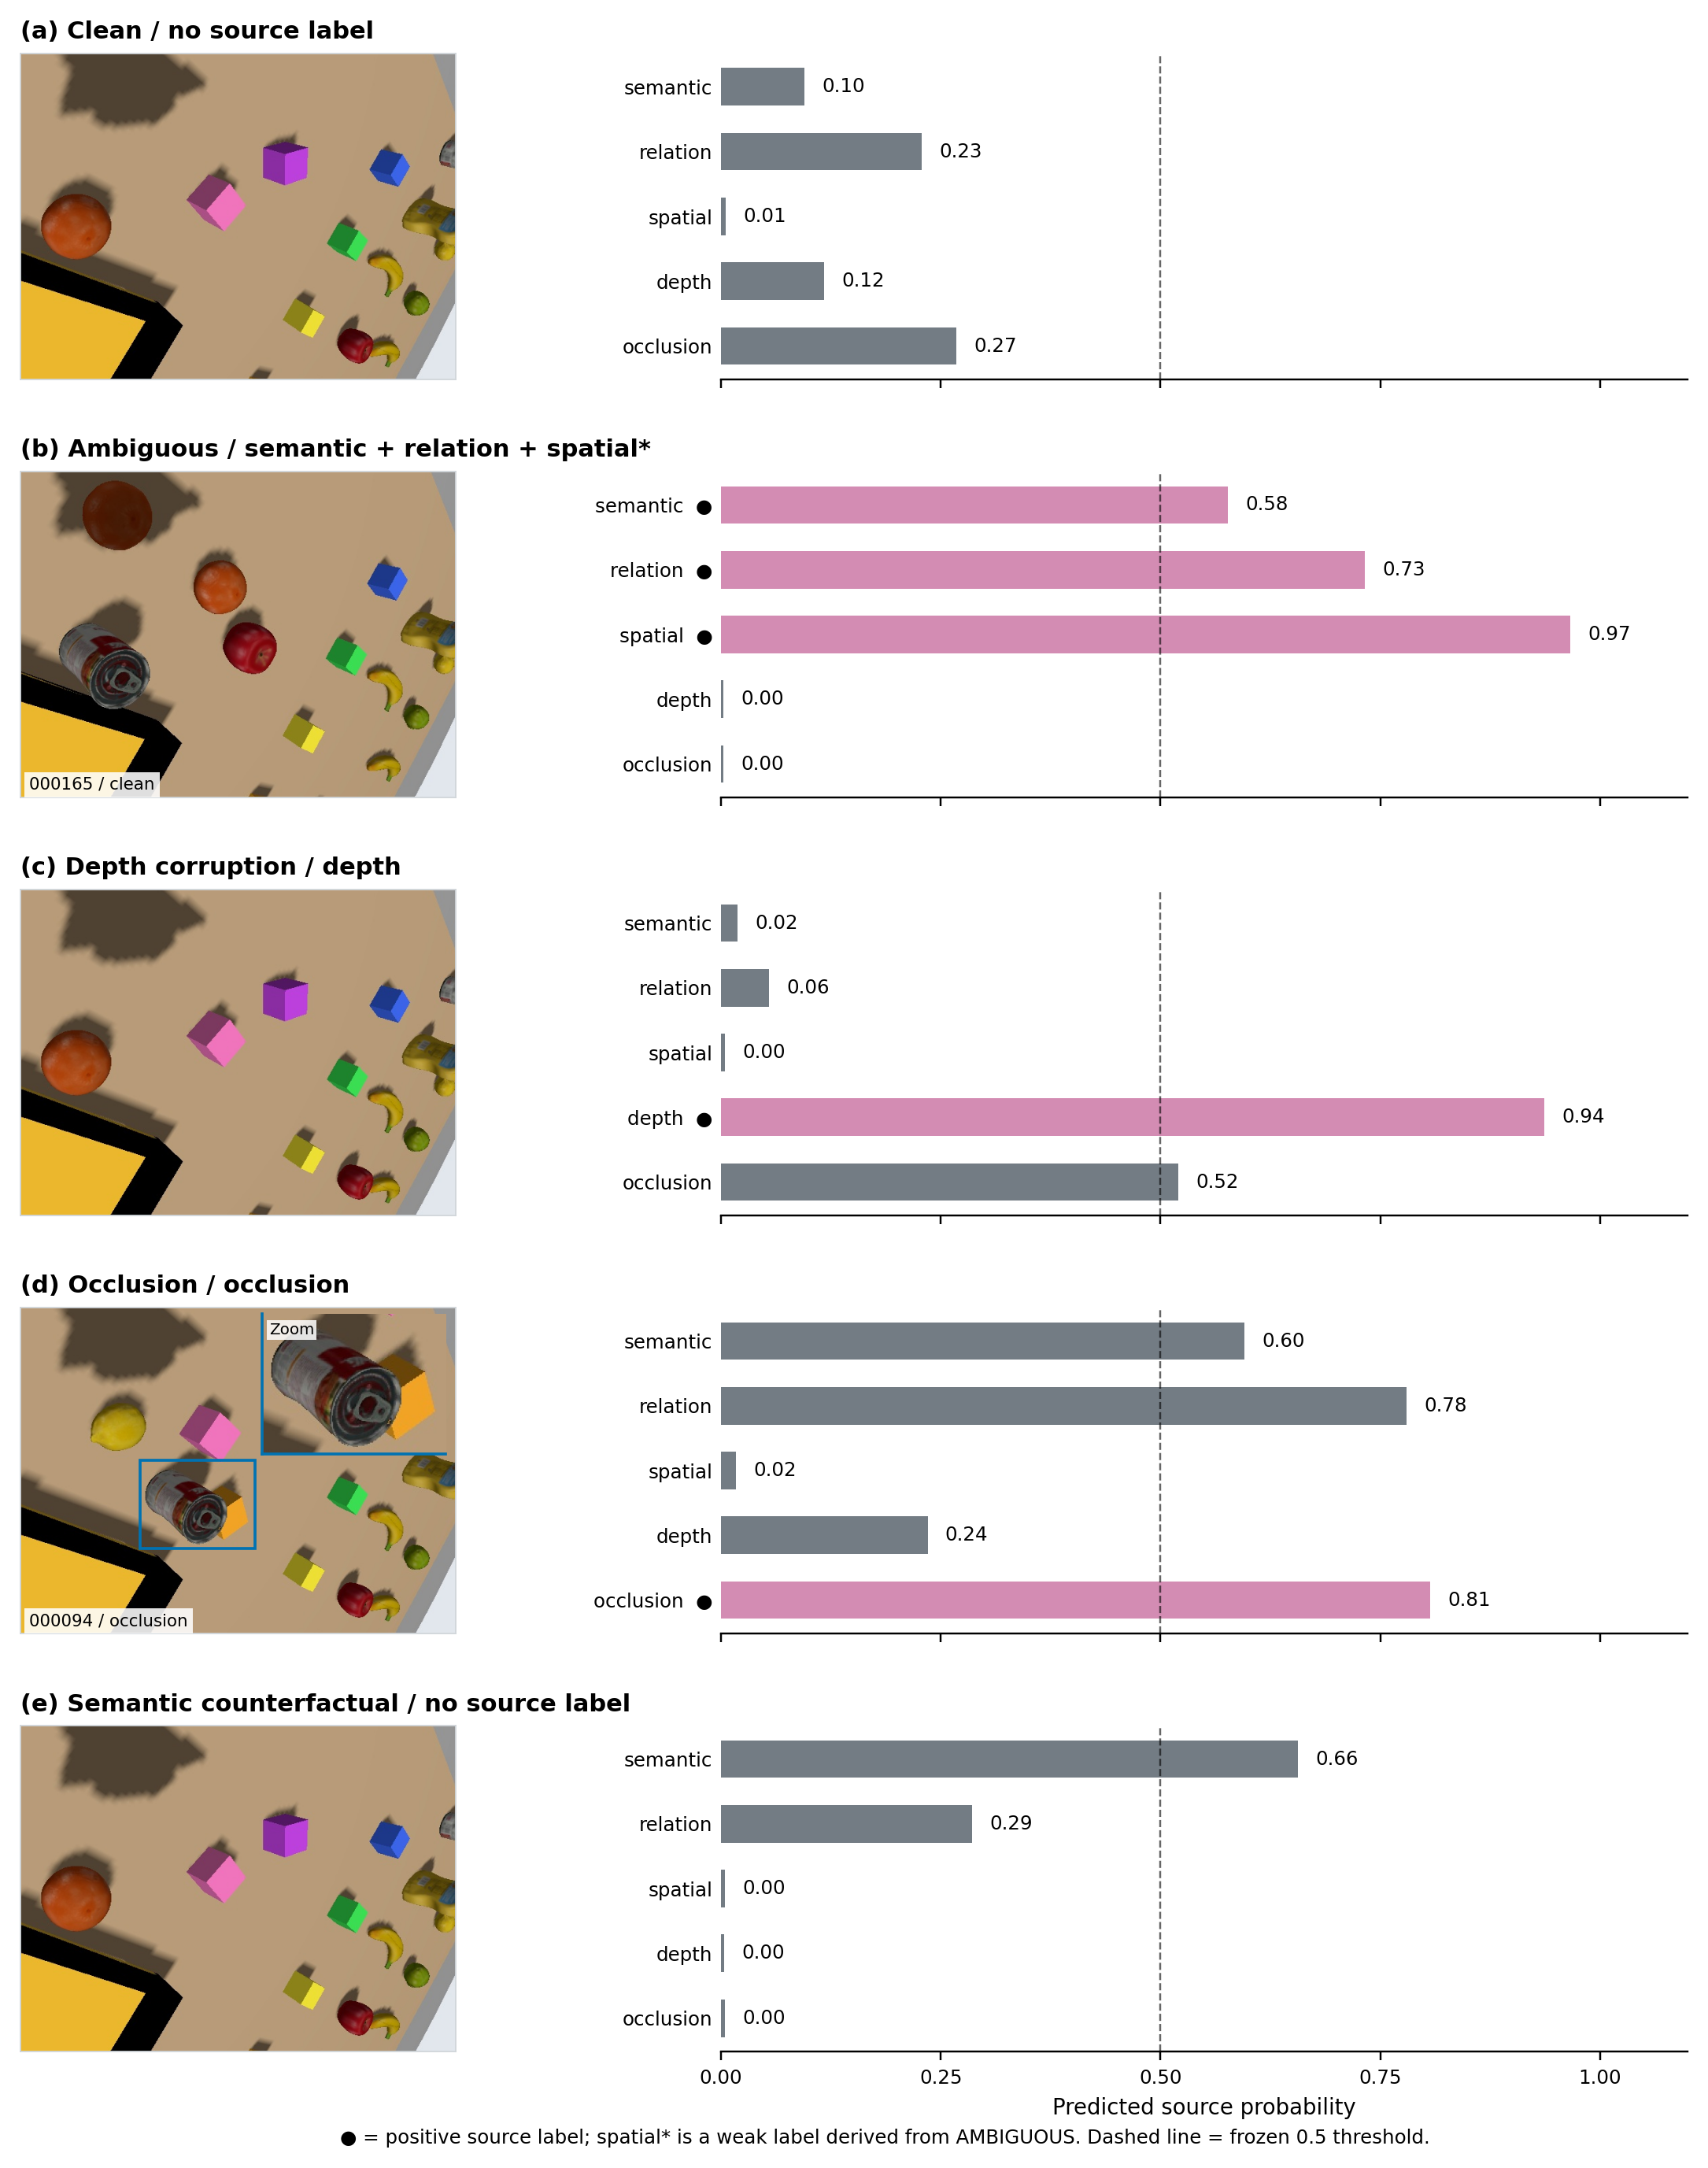
\includegraphics[width=\textwidth,height=0.72\textheight,keepaspectratio]{hinhanh/fig08_source_uncertainty_cases.png}
    \caption{Source scores từ prediction Test-IID đã khóa:
    (a), (c), (e) thuộc family 127; (b) là sample
    \texttt{v211iid\_\allowbreak family\_\allowbreak 000165\_\allowbreak \_\allowbreak clean} mơ hồ,
    với score spatial thực 0.9659 (hiển thị 0.97);
    (d) là sample \texttt{v211iid\_\allowbreak family\_\allowbreak 000094\_\allowbreak \_\allowbreak occlusion\_\allowbreak view\_\allowbreak counterfactual},
    trong đó hộp súp che một phần khối lập phương màu cam.
    Ô phóng to ở (d) lấy từ cùng ảnh RGB; score occlusion
    là 0.8069 (hiển thị 0.81). Ký hiệu nhãn dương chỉ phục
    vụ evaluator; spatial là nhãn yếu suy từ AMBIGUOUS.
    Variant semantic của family 127 có false positive
    semantic dù target vẫn FOUND.}
    \label{fig:results-source-cases}
    {\footnotesize Nguồn: RGB Gazebo, source prediction
    và nhãn thật của Test-IID; threshold hiển thị 0.5.\par}
\end{figure}

Hình~\ref{fig:results-demo-source-occlusion} tách hai cách nhìn
về che khuất. Trên ảnh camera, chai mù tạt che một phần hộp súp;
trong bố trí mặt bàn, hai vật có footprint tách nhau. Đây là
minh họa một sample, không phải phép đánh giá độ chính xác
hình học hoặc source head trên toàn tập.

\begin{figure}[htbp]
    \centering
    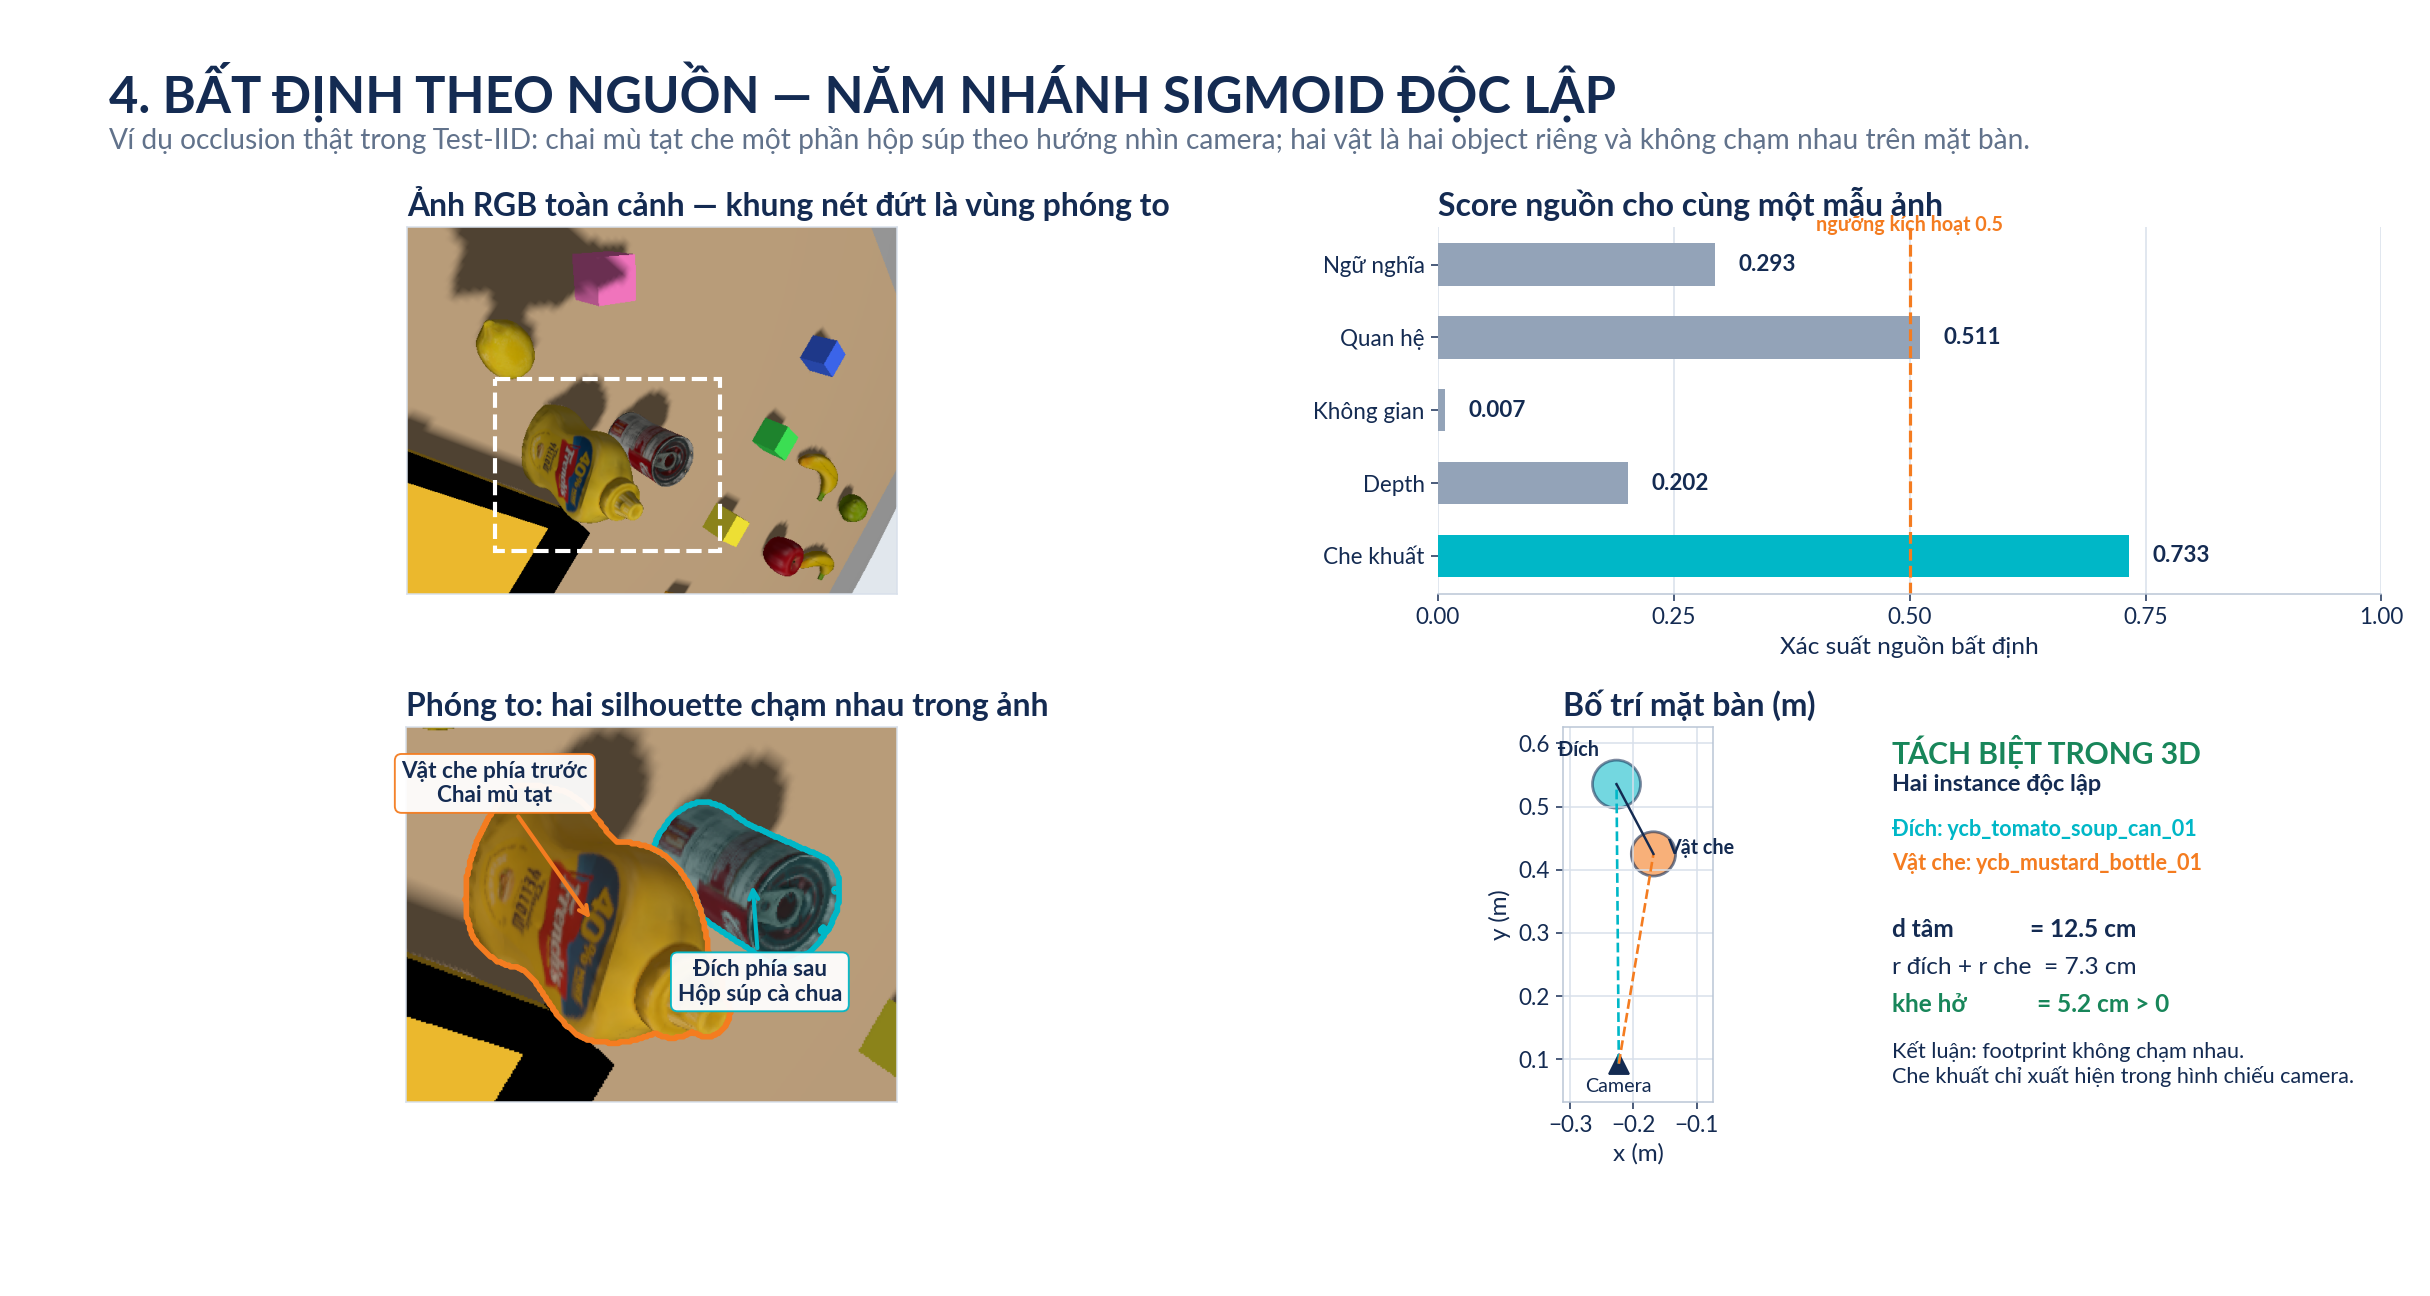
\includegraphics[width=\textwidth,height=0.68\textheight,keepaspectratio]{hinhanh/04_bat_dinh_theo_nguon.png}
    \caption{Năm score source trên sample
    \texttt{v211iid\_\allowbreak family\_\allowbreak 000113\_\allowbreak \_\allowbreak occlusion\_\allowbreak view\_\allowbreak counterfactual}.
    Nhãn chuẩn source là occlusion; score occlusion 0.733 và
    relation 0.511 cùng vượt ngưỡng 0.5. Chai mù tạt che hộp
    súp trong hình chiếu camera, còn khoảng hở giữa hai
    footprint theo layout là 5.2 cm. Mask và semantic label
    chỉ dùng để chú giải sau suy luận.}
    \label{fig:results-demo-source-occlusion}
\end{figure}

\begin{figure}[htbp]
    \centering
    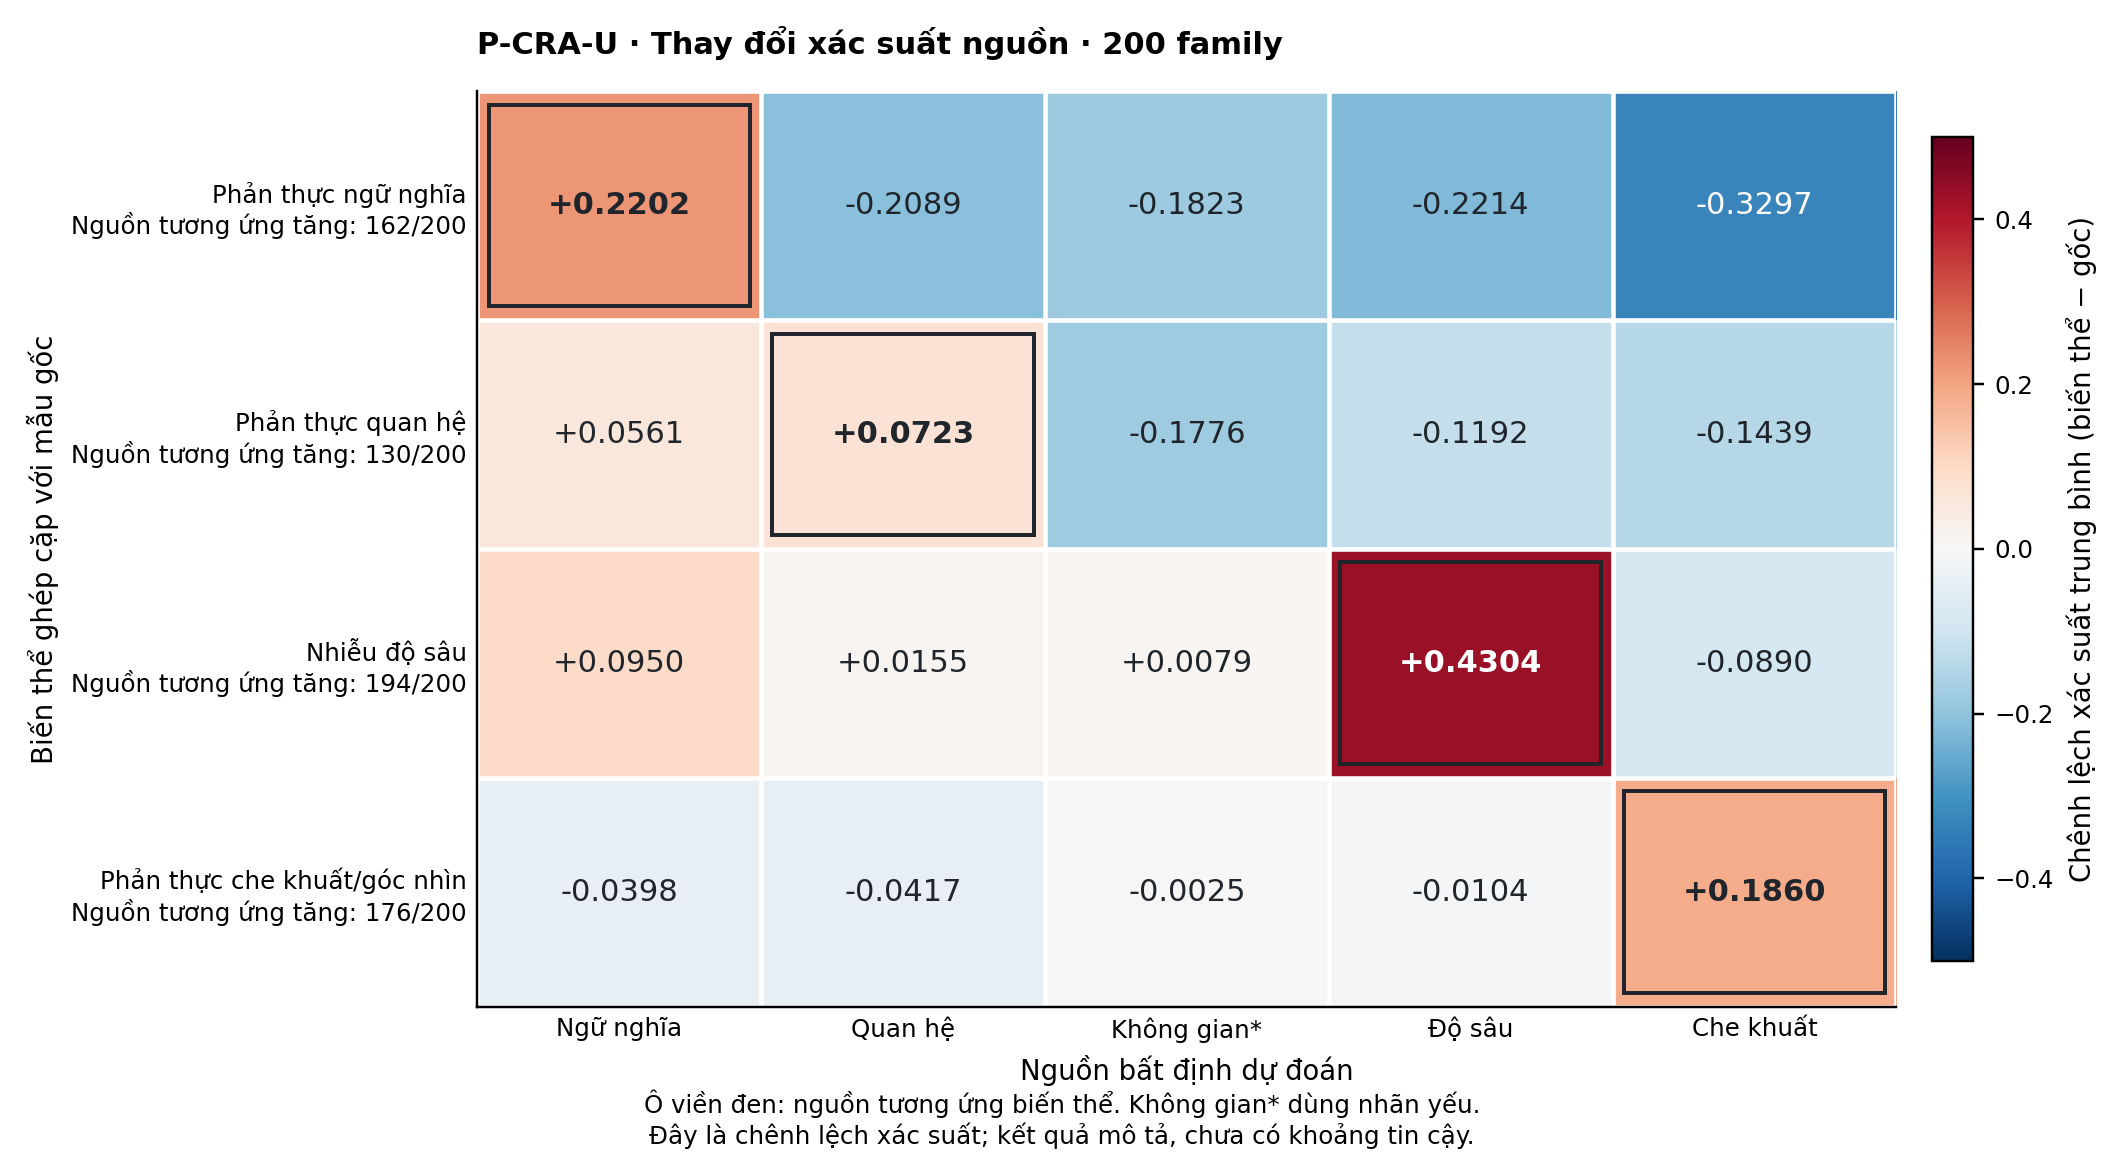
\includegraphics[width=\textwidth,height=0.58\textheight,keepaspectratio]{hinhanh/fig21_pcrau_paired_source_delta_adapter_vi.png}
    \caption{Phản ứng paired của source uncertainty
    P-CRA-U: mỗi ô là trung bình $\Delta u_s$
    giữa variant và clean trên 200 cặp family.
    Màu đỏ biểu thị tăng, xanh biểu thị giảm xác suất;
    ô viền đen là source cùng tên loại can thiệp.
    Số cạnh hàng đếm cặp có source tương ứng tăng.
    Spatial$^*$ dùng nhãn yếu; không xem heatmap này
    là bằng chứng attribution nhân quả. Số liệu khớp
    Bảng~\ref{tab:results-source-delta}, chưa có CI.}
    \label{fig:results-source-delta-pending}
    {\footnotesize Nguồn: \texttt{source\_\allowbreak probabilities}
    trong \texttt{predictions.jsonl}, ghép clean--variant
    theo family ID; dựng bằng Matplotlib, không suy luận lại.\par}
\end{figure}

Top-1 source accuracy chưa được báo vì nhãn là đa
nhãn và có sample không source dương. Cần định nghĩa
rõ cách chấm trong hai trường hợp này trước khi
bổ sung, không thay đa nhãn F1 bằng argmax tùy ý.

\section{Đánh giá calibration}
\label{sec:results-calibration}

\subsection{Score tham chiếu và risk đã hiệu chuẩn}

Score tham chiếu của mỗi phiên bản là $r_{\rm raw}=1-p(\mathrm{FOUND})$
từ chính answerability head tương ứng. Risk V2 dùng logistic18;
P-CRA-U hiện tại dùng logistic33 fit sau khi đóng băng Adapter.
Bảng tách rõ phiên bản, tránh dùng raw score cũ làm mốc của head mới.

\begin{table}[htbp]
    \centering
    \setlength{\tabcolsep}{4pt}
    \renewcommand{\arraystretch}{1.15}
    \caption{Chất lượng risk trên cùng 1000 mẫu, với cùng biến cố lỗi.}
    \label{tab:results-calibration-comparison}
    \small
    \begin{tabularx}{\textwidth}{@{}>{\raggedright\arraybackslash}Xrrrrrr@{}}
        \toprule
        Score & \shortstack{AUROC\\$\uparrow$} & \shortstack{AP\\$\uparrow$} &
        \shortstack{Brier\\$\downarrow$} & \shortstack{NLL\\$\downarrow$} &
        \shortstack{ECE$_{10}$\\$\downarrow$} & \shortstack{AURC\\$\downarrow$} \\
        \midrule
        V2: raw & 0.94416 & 0.96223 & 0.10355 & 0.33439 & 0.07203 & 0.26256 \\
        V2: logistic18 & 0.94546 & 0.96202 & 0.09615 & 0.29848 & 0.04647 & 0.26045 \\
        \midrule
        Adapter: raw & 0.96361 & 0.97601 & 0.08014 & 0.25919 & 0.04847 & 0.25140 \\
        Adapter: logistic33 & 0.95957 & 0.96741 & 0.07711 & 0.25707 & 0.03108 & 0.25575 \\
        \bottomrule
    \end{tabularx}
    {\footnotesize\raggedright Nguồn: artifact V2, prediction và runtime decision
    Adapter; raw là $1-p(\mathrm{FOUND})$ của từng phiên bản.
    Cùng quy tắc metric, không fit bằng test. Chưa có scalar-only đã fit
    để cô lập lợi ích hiệu chuẩn khỏi lợi ích thêm evidence.\par}
\end{table}

Hình~\ref{fig:results-demo-calibrated-risk} nối score risk
với bốn hành động trên những sample cụ thể. Chỉ mẫu FOUND
có risk dưới ngưỡng đã khóa đi đến EXECUTE; các trạng thái
còn lại cần quyết định phù hợp với answerability và evidence.

\begin{figure}[htbp]
    \centering
    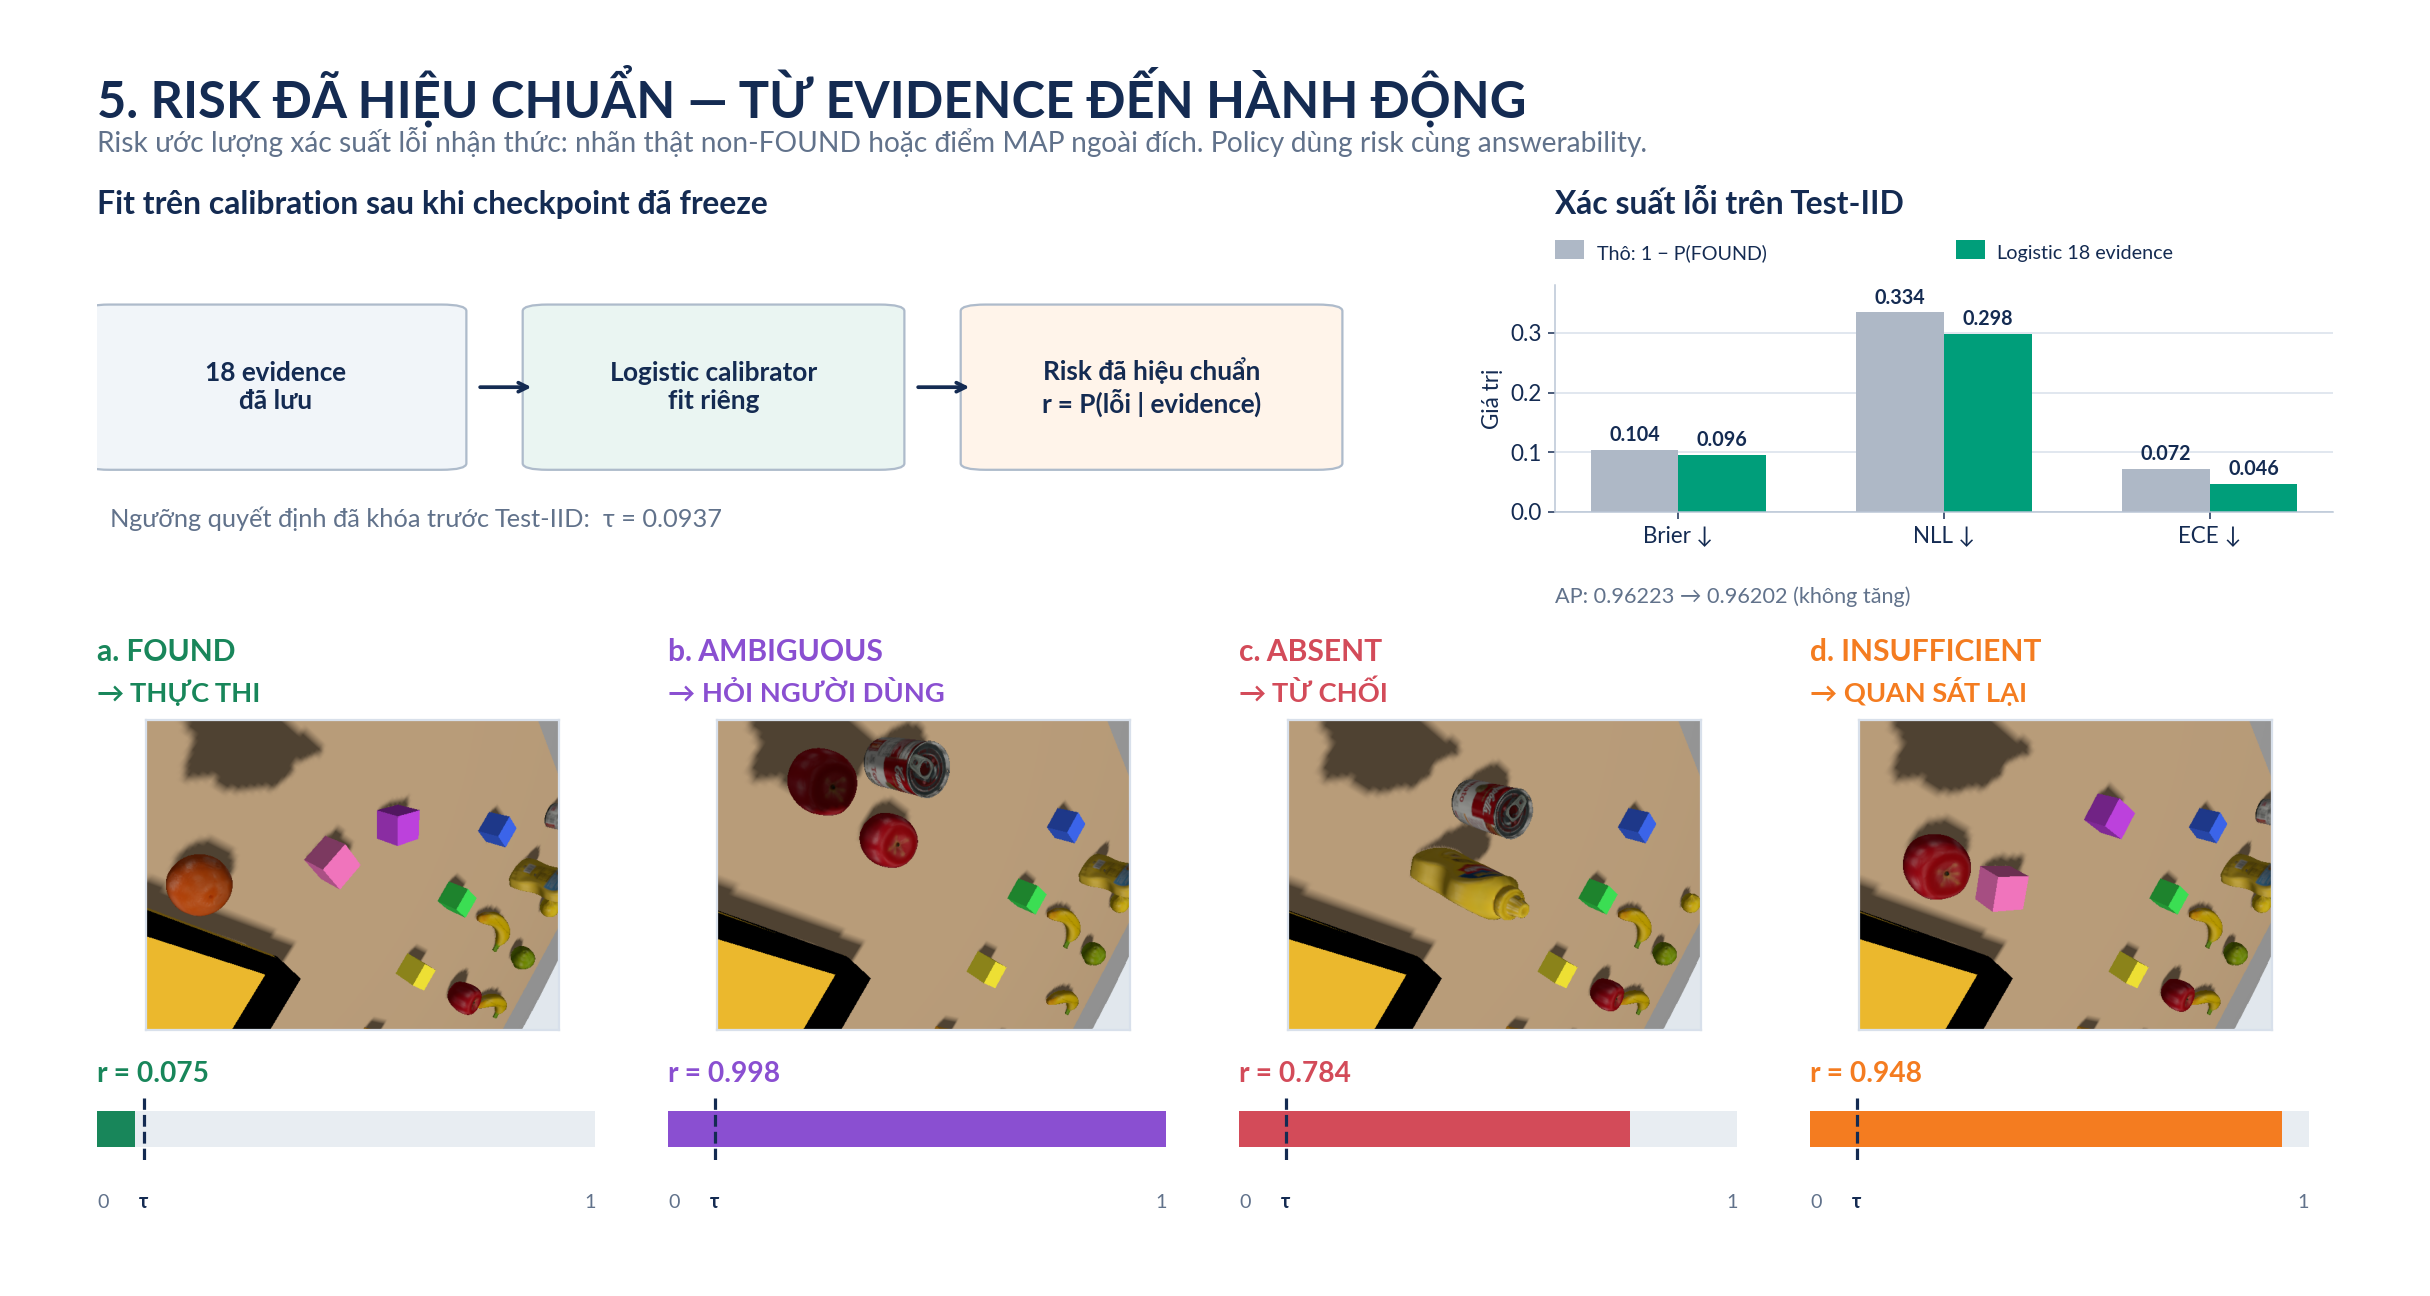
\includegraphics[width=\textwidth,height=0.68\textheight,keepaspectratio]{hinhanh/05_risk_da_hieu_chuan.png}
    \caption{Minh họa V2 lịch sử: logistic calibrator 18 evidence và
    risk trên bốn sample Test-IID. Ngưỡng $\tau=0.0937$ được
    chọn trước test; các cột Brier, NLL và ECE so sánh
    $1-p(\mathrm{FOUND})$ với risk đã hiệu chuẩn. Risk là ước
    lượng của biến cố lỗi nhận thức ở
    Công thức~\eqref{eq:results-risk-event}, không phải xác
    suất robot thao tác thất bại.}
    \label{fig:results-demo-calibrated-risk}
\end{figure}

Với Adapter, logistic33 giảm Brier từ 0.08014 xuống 0.07711,
NLL từ 0.25919 xuống 0.25707 và ECE từ 0.04847 xuống 0.03108
so với raw score cùng head. Tuy nhiên, AUROC/AP thấp hơn raw,
AURC tăng từ 0.25140 lên 0.25575: hiệu chuẩn xác suất và ranking
là hai tiêu chí khác nhau, không phải mọi chỉ số đều cải thiện.
So với logistic18 V2 lịch sử, logistic33 có Brier/NLL/ECE và AURC
tốt hơn, nhưng phép so sánh đồng thời thay answerability và evidence;
chưa quy phần cải thiện riêng cho source hoặc bước fit xác suất.

Phần lớn biến cố lỗi là non-FOUND. Chất lượng risk tổng không xác nhận
ranking riêng của 15 điểm sai trên FOUND. Chưa có CI family cho mọi
chênh lệch Brier/NLL/ECE, nên các giá trị là thống kê mô tả.
Hình demo risk 18 evidence được giữ như minh họa V2 lịch sử;
reliability và risk--coverage bên dưới dùng kết quả Adapter hiện tại.

\subsection{Reliability diagram}

ECE dùng 10 bin độ rộng bằng nhau. Trục tung
của Hình~\ref{fig:results-reliability} là tỉ
lệ lỗi quan sát, không phải accuracy; đường
chéo biểu thị risk bằng tần suất lỗi.
Kích thước marker phản ánh số sample trong
bin, giúp phân biệt bin ít quan sát với bin
có nhiều bằng chứng.

\begin{figure}[htbp]
    \centering
    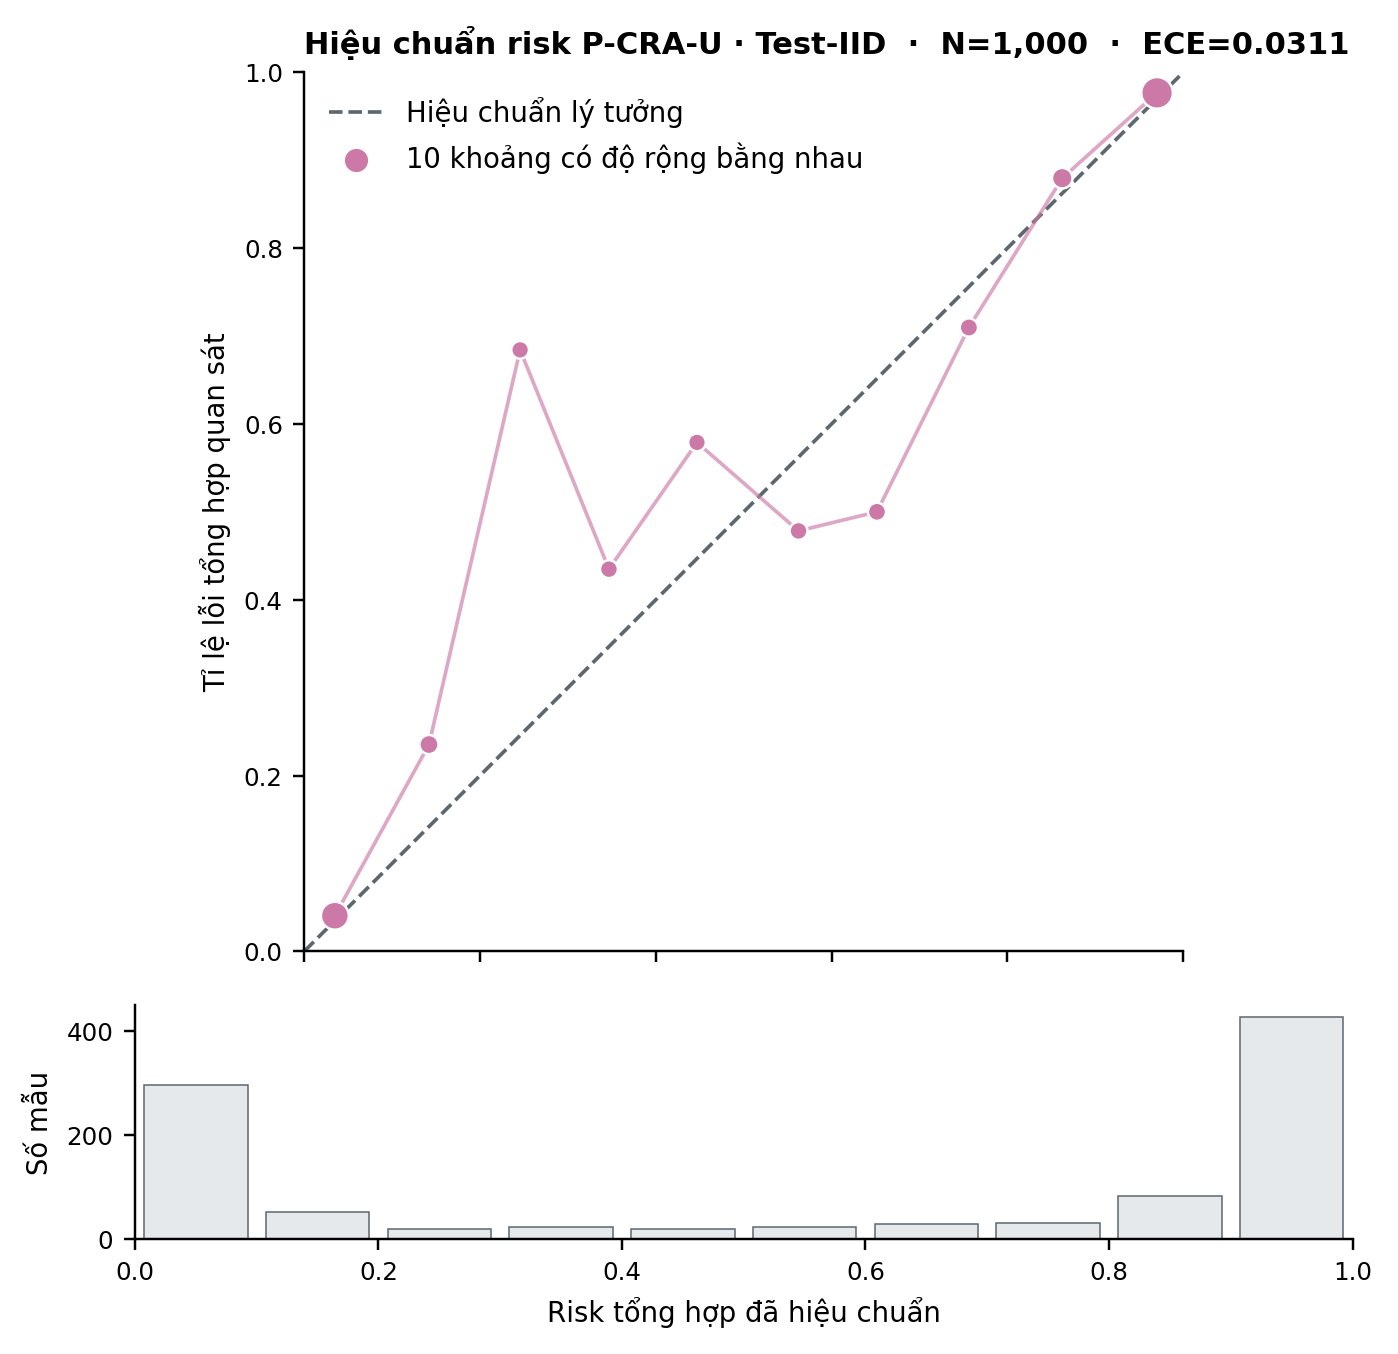
\includegraphics[width=\textwidth,height=0.62\textheight,keepaspectratio]{hinhanh/fig10_reliability_test_iid_adapter_vi.png}
    \caption{Reliability diagram của risk Adapter trên Test-IID,
    với 10 bin và ECE 0.03108. Marker biểu thị quy mô bin;
    đường chéo là hiệu chuẩn lý tưởng của xác suất lỗi.}
    \label{fig:results-reliability}
    {\footnotesize Nguồn: calibrated risk và error event
    thật của 1000 sample Test-IID.\par}
\end{figure}

ECE nhỏ không đồng nghĩa mọi phân tầng đều
được hiệu chuẩn tốt. Những bin ít mẫu hoặc
nhóm box bị hồi quy cần phân tích riêng.
Chưa có CI theo family cho ECE/Brier/NLL,
nên các khác biệt ở bảng calibration là
ước lượng điểm, không phải kết luận kiểm
định thống kê tương ứng.

\subsection{Risk--coverage và điểm vận hành}

Đường risk--coverage nhận dần sample theo
risk tăng dần. AURC tích lũy rủi ro trên
nhiều mức coverage, còn threshold đóng băng
xác định một điểm vận hành.
Profile Adapter khóa $\tau=0.2611932835$ và cổng FOUND, chấp nhận
361/1000 mẫu với 34 lỗi: coverage 36.10\%, selective risk 9.42\%.
Đường cong nhận dần cả 1000 mẫu theo risk; điểm policy có thêm cổng
answerability nên không nhất thiết nằm đúng trên đường risk-only.
Ở ngưỡng này, risk-only nhận 362 mẫu, còn policy nhận 361 mẫu.

\begin{figure}[htbp]
    \centering
    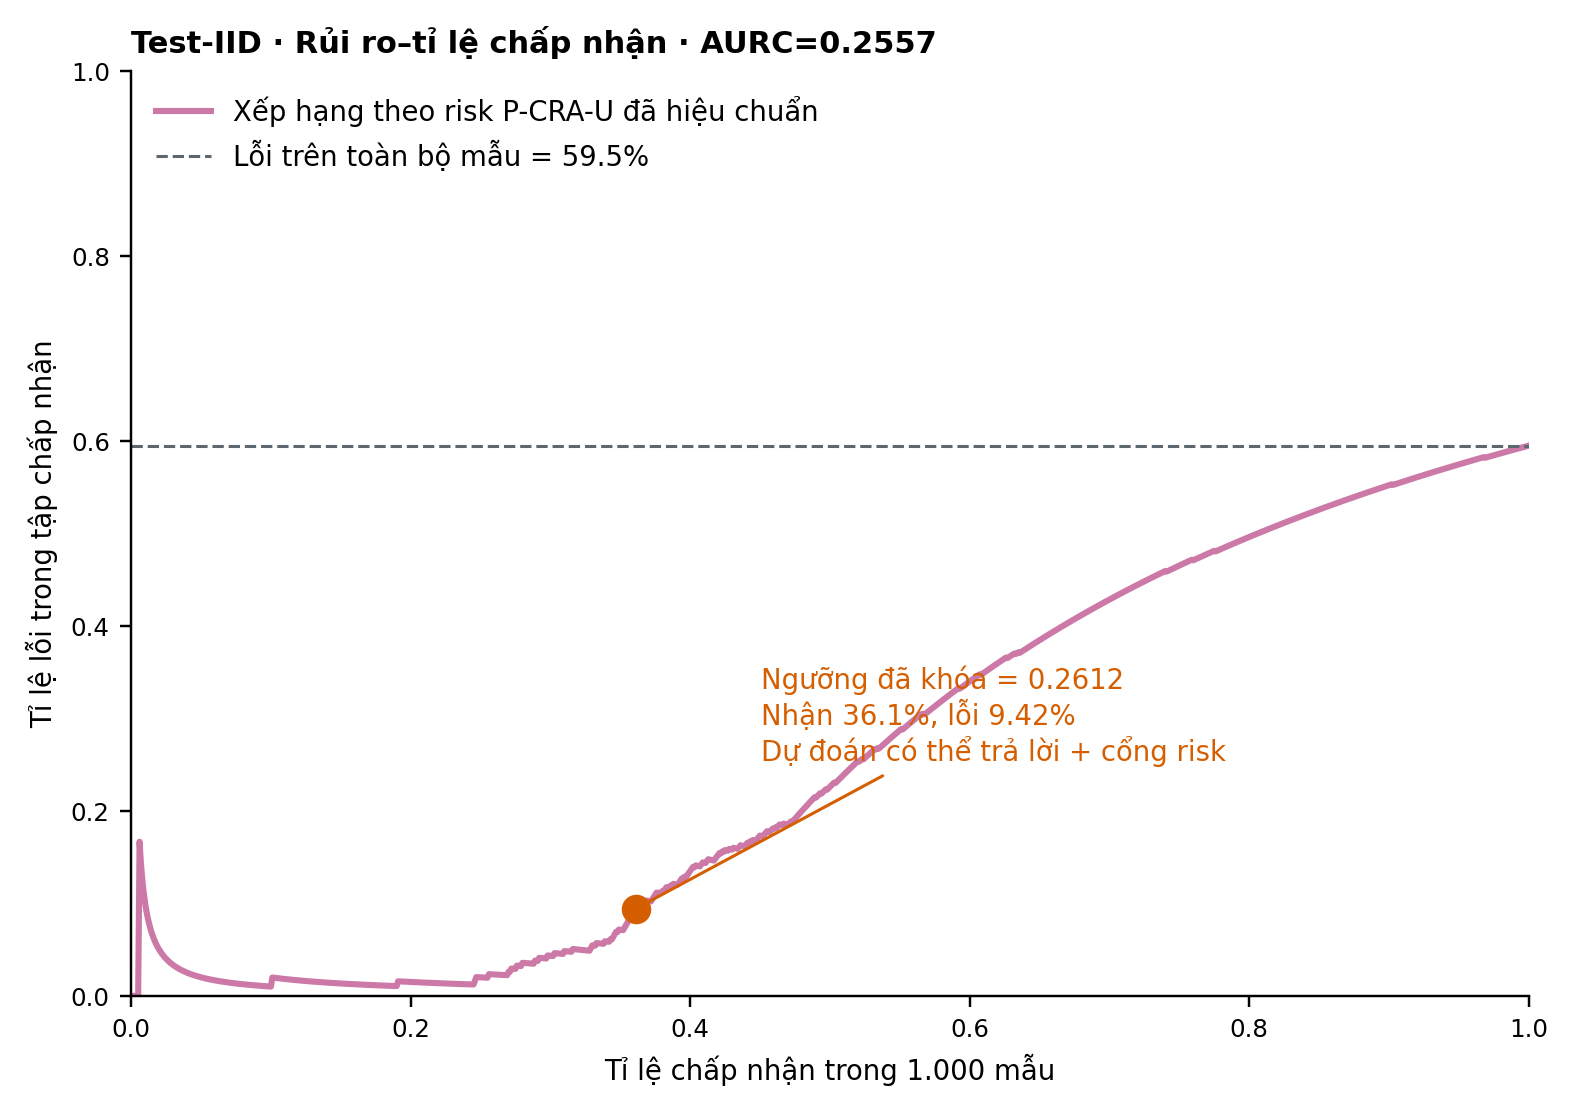
\includegraphics[width=\textwidth,height=0.62\textheight,keepaspectratio]{hinhanh/fig11_risk_coverage_test_iid_adapter_vi.png}
    \caption{Risk--coverage của Adapter trên Test-IID cũ.
    AURC risk-only là 0.25575; điểm policy hard-FOUND có coverage
    36.10\% và selective risk 9.42\%. Ngân sách chọn ngưỡng trên
    calibration là 7.5\%, không phải lỗi test đã đạt 7.5\%.}
    \label{fig:results-risk-coverage}
    {\footnotesize Nguồn: prediction, runtime risk và ngưỡng khóa
    của Adapter; không chọn lại ngưỡng theo test.\par}
\end{figure}

AURC cần đọc cùng prevalence lỗi 0.595. Ngay cả thứ tự oracle nhận
405 ca đúng trước cũng có AURC 0.22923 vì phải nhận thêm 595 ca lỗi
khi coverage tiến tới 100\%. Adapter có excess-AURC 0.02652,
giảm từ 0.03122 của V2; không dùng ngưỡng tùy ý AURC $<0.1$ cho
biến cố và phân bố này. AURC không phụ thuộc riêng mốc ngân sách
5\%, 7.5\% hay 10\%; mỗi mốc chỉ chọn một điểm vận hành.
Ngược lại, AURC tổng chưa bảo đảm risk thấp ở đúng vùng hành động.

{\setlength{\emergencystretch}{3em}
CI 95\% cluster theo 200 family của selective risk là
$[6.37,12.53]\%$. Coverage có CI $[33.80,38.40]\%$.
Lỗi điểm 9.42\% vượt ngân sách 7.5\%; cận Wilson theo sample là
12.87\%. Mức vận hành được chọn chấp nhận đánh đổi thực nghiệm này
để tăng số ca đúng được nhận, không có bảo đảm lỗi dưới 7.5\%
hoặc dưới 10\% trên phân bố mới. Bootstrap giữ ngưỡng đã khóa;
không chọn lại ngưỡng trong từng lượt hoặc bằng số liệu test.\par}


\section{Vùng tin cậy không gian}
\label{sec:results-region}

\subsection{Coverage và kích thước vùng}

Vùng highest-density dùng $\alpha=0.1$ và
frozen probability mass 0.6041832. Mức nominal
coverage là 90\%, còn Test-IID đạt 86.83\%
theo score evaluator đã khai báo. Hai đại
lượng không đồng nhất; mass 0.60418 không
phải nominal coverage 60.42\%.

\begin{table}[htbp]
    \centering
    \setlength{\tabcolsep}{4pt}
    \renewcommand{\arraystretch}{1.15}
    \caption{Vùng highest-density kế thừa V2 của P-CRA-U trên 835 sample
    có target, dùng threshold fit trước test.}
    \label{tab:results-region}
    \small
    \begin{tabularx}{\textwidth}{@{}>{\raggedright\arraybackslash}Xr>{\raggedright\arraybackslash}X@{}}
        \toprule
        Đại lượng & Giá trị & Ý nghĩa \\
        \midrule
        $\alpha$ & 0.10 & Mức lỗi mục tiêu của thiết kế \\
        Nominal coverage (\%) & 90.00 & $1-\alpha$ \\
        Frozen probability mass & 0.6041832 & Tham số fit trên calibration \\
        Empirical coverage (\%) & 86.83 & 725/835 sample theo score \\
        Coverage gap (pp) & $-3.17$ & Empirical trừ nominal \\
        Diện tích lưới trung bình (\%) & 0.5194 & Tỉ lệ ô region / 768 ô \\
        Diện tích lưới trung vị (\%) & 0.5208 & Tương ứng 4/768 ô \\
        \bottomrule
    \end{tabularx}
    \vspace{2pt}
    {\footnotesize\raggedright Nguồn: \texttt{conformal\_\allowbreak spatial\_\allowbreak region}
    trong \texttt{full\_\allowbreak metrics.json}. Diện tích không phải
    diện tích bounding box; chưa có CI cho coverage.\par}
\end{table}

Vùng nhỏ, trung vị bốn ô, có thể thuận tiện
để hiển thị một ứng viên compact. Tuy nhiên,
110/835 sample chưa đạt event coverage theo
score; empirical thấp hơn nominal 3.17 pp.
Không công bố hệ thống đã đạt bảo đảm 90\%
chỉ vì cấu hình đặt $\alpha=0.1$.

\subsection{Quy tắc rời rạc và cách đọc hình}

Evaluator hiện chấm $S_i\leq m_\alpha$, với
$S_i$ là khối lượng tích lũy đến ô target
đầu tiên trong thứ tự xác suất. Region hiển
thị lấy các ô đến khi đạt hoặc vượt mass.
Ở biên lưới rời rạc, score event không nhất
thiết đồng nhất hoàn toàn với kiểm tra giao
tập ô và mask. Số liệu trong bảng giữ đúng
event đã lưu, không đổi định nghĩa coverage.

\begin{figure}[htbp]
    \centering
    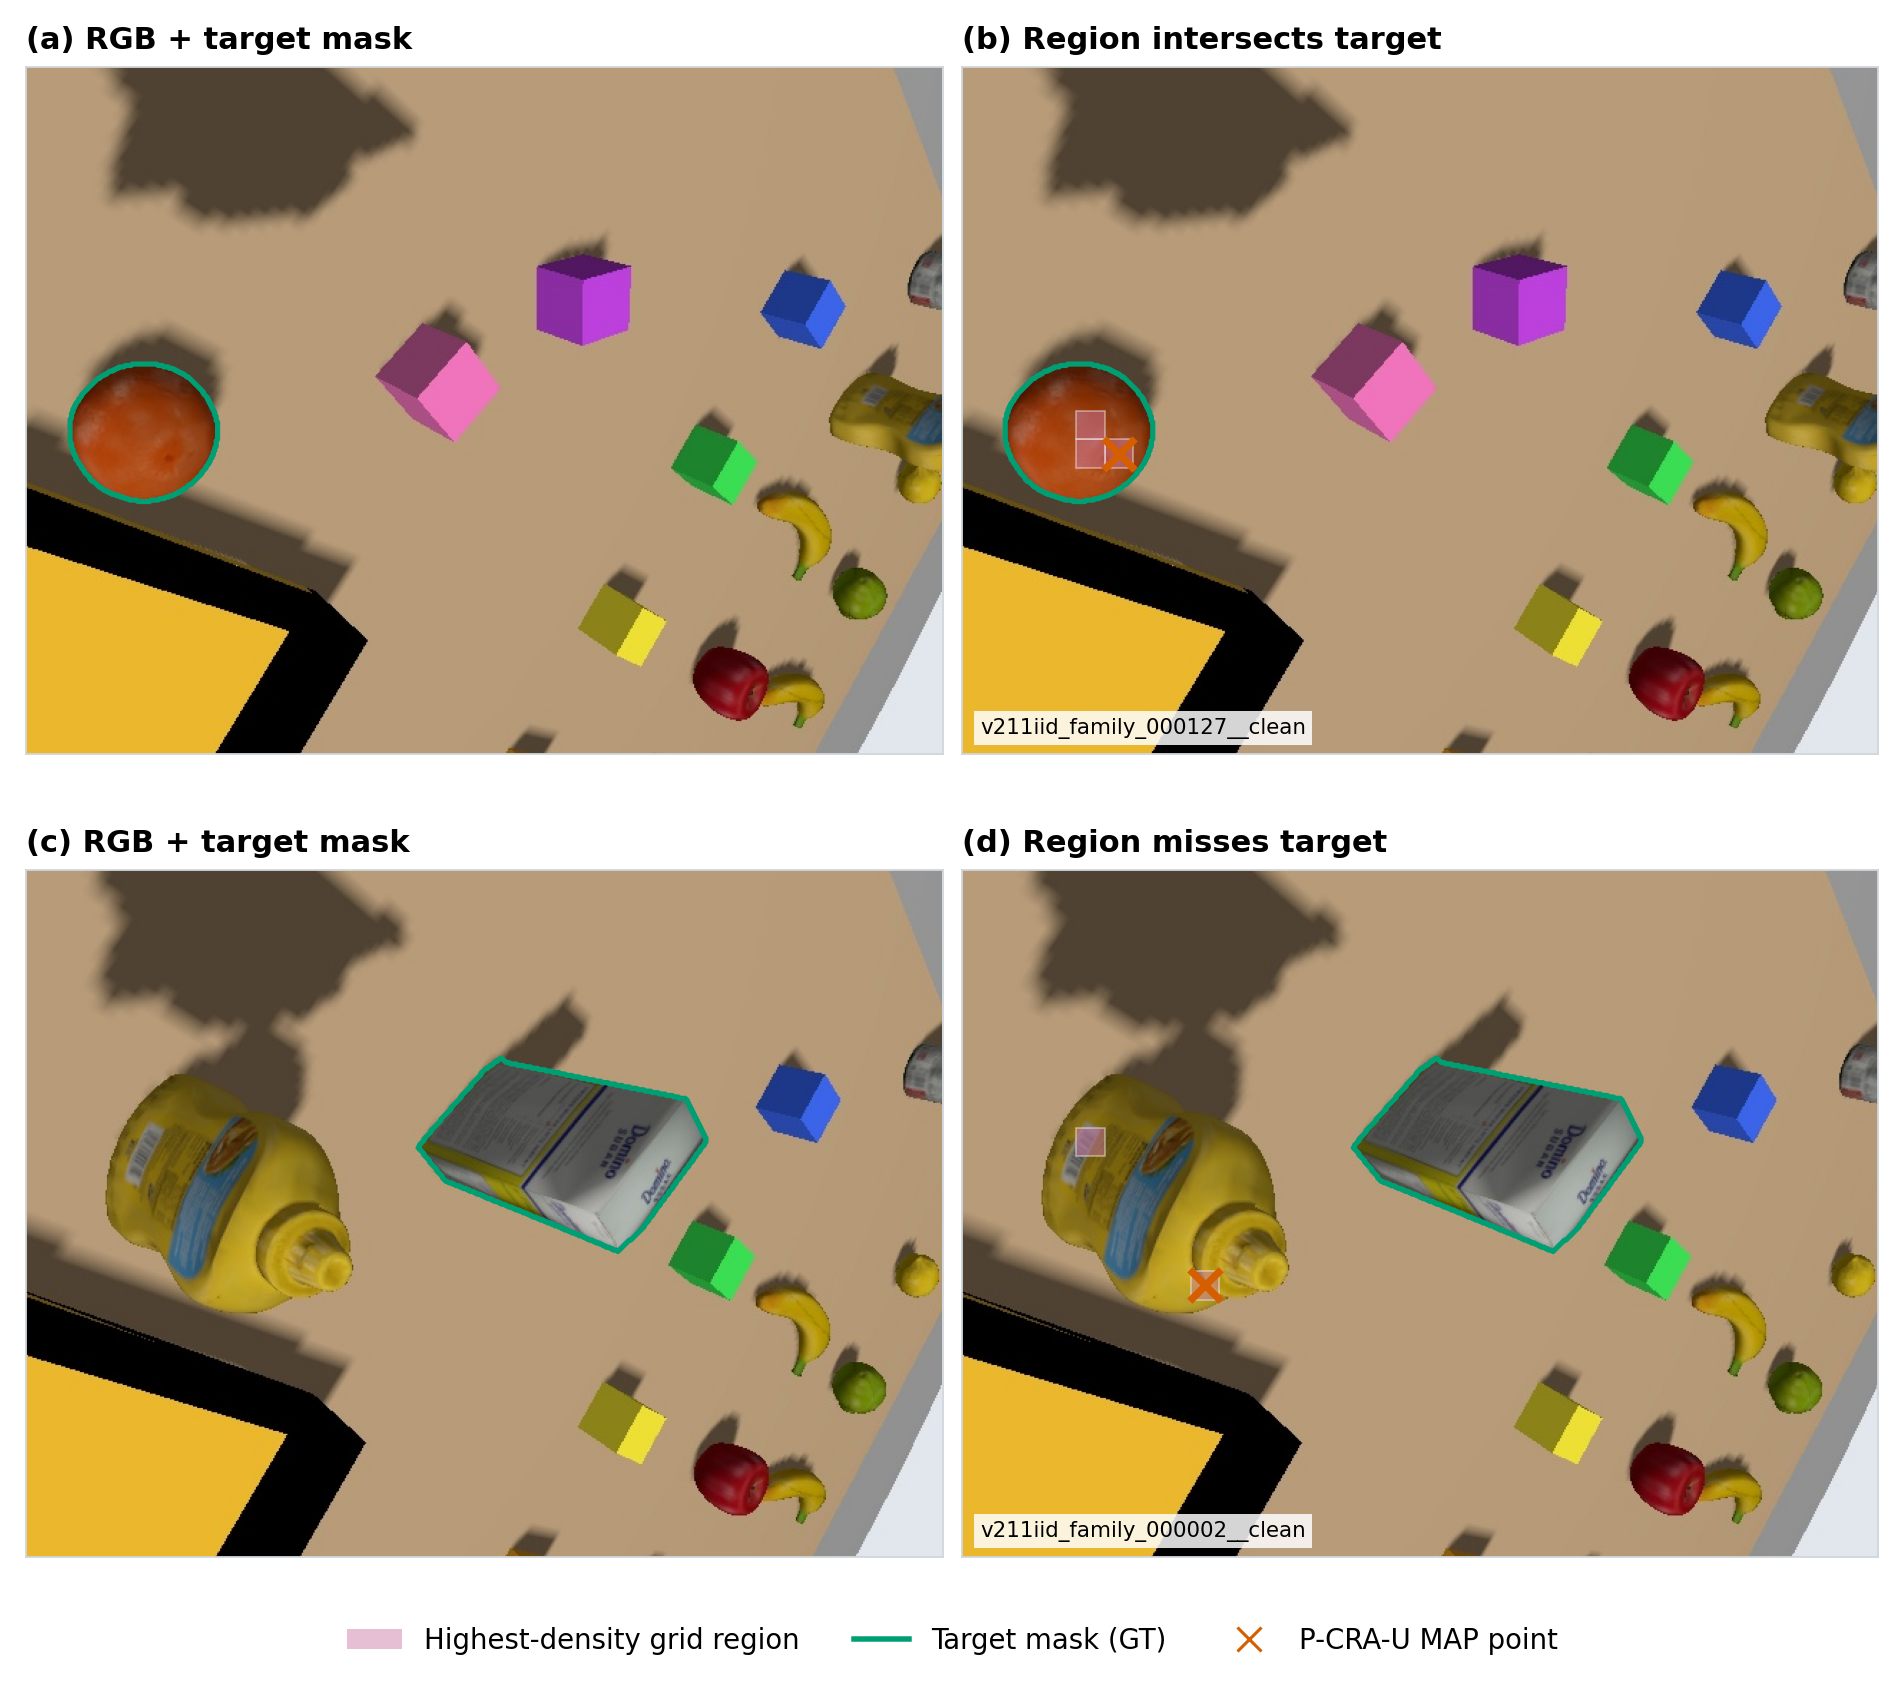
\includegraphics[width=\textwidth,height=0.65\textheight,keepaspectratio]{hinhanh/fig12_confidence_region_true_rgb.png}
    \caption{Vùng highest-density trên RGB của hai sample:
    family 127 clean là ví dụ vùng chạm target, family
    002 clean là ví dụ bỏ lỡ target. Vùng được dựng từ
    prediction, không chỉnh tay theo mask.}
    \label{fig:results-confidence-region}
    {\footnotesize Nguồn: probability grid V2, frozen mass
    và evaluator Test-IID; mask target chỉ dùng hậu kiểm.\par}
\end{figure}

Hình~\ref{fig:results-demo-spatial-region} phóng to vùng
highest-density của chính sample mơ hồ ở
Hình~\ref{fig:results-demo-spatial-distribution}. Vùng có thể
gồm các ô rời nhau và chứa MAP ứng viên, nhưng không giải
quyết thay answerability để cấp quyền thực thi.

\begin{figure}[htbp]
    \centering
    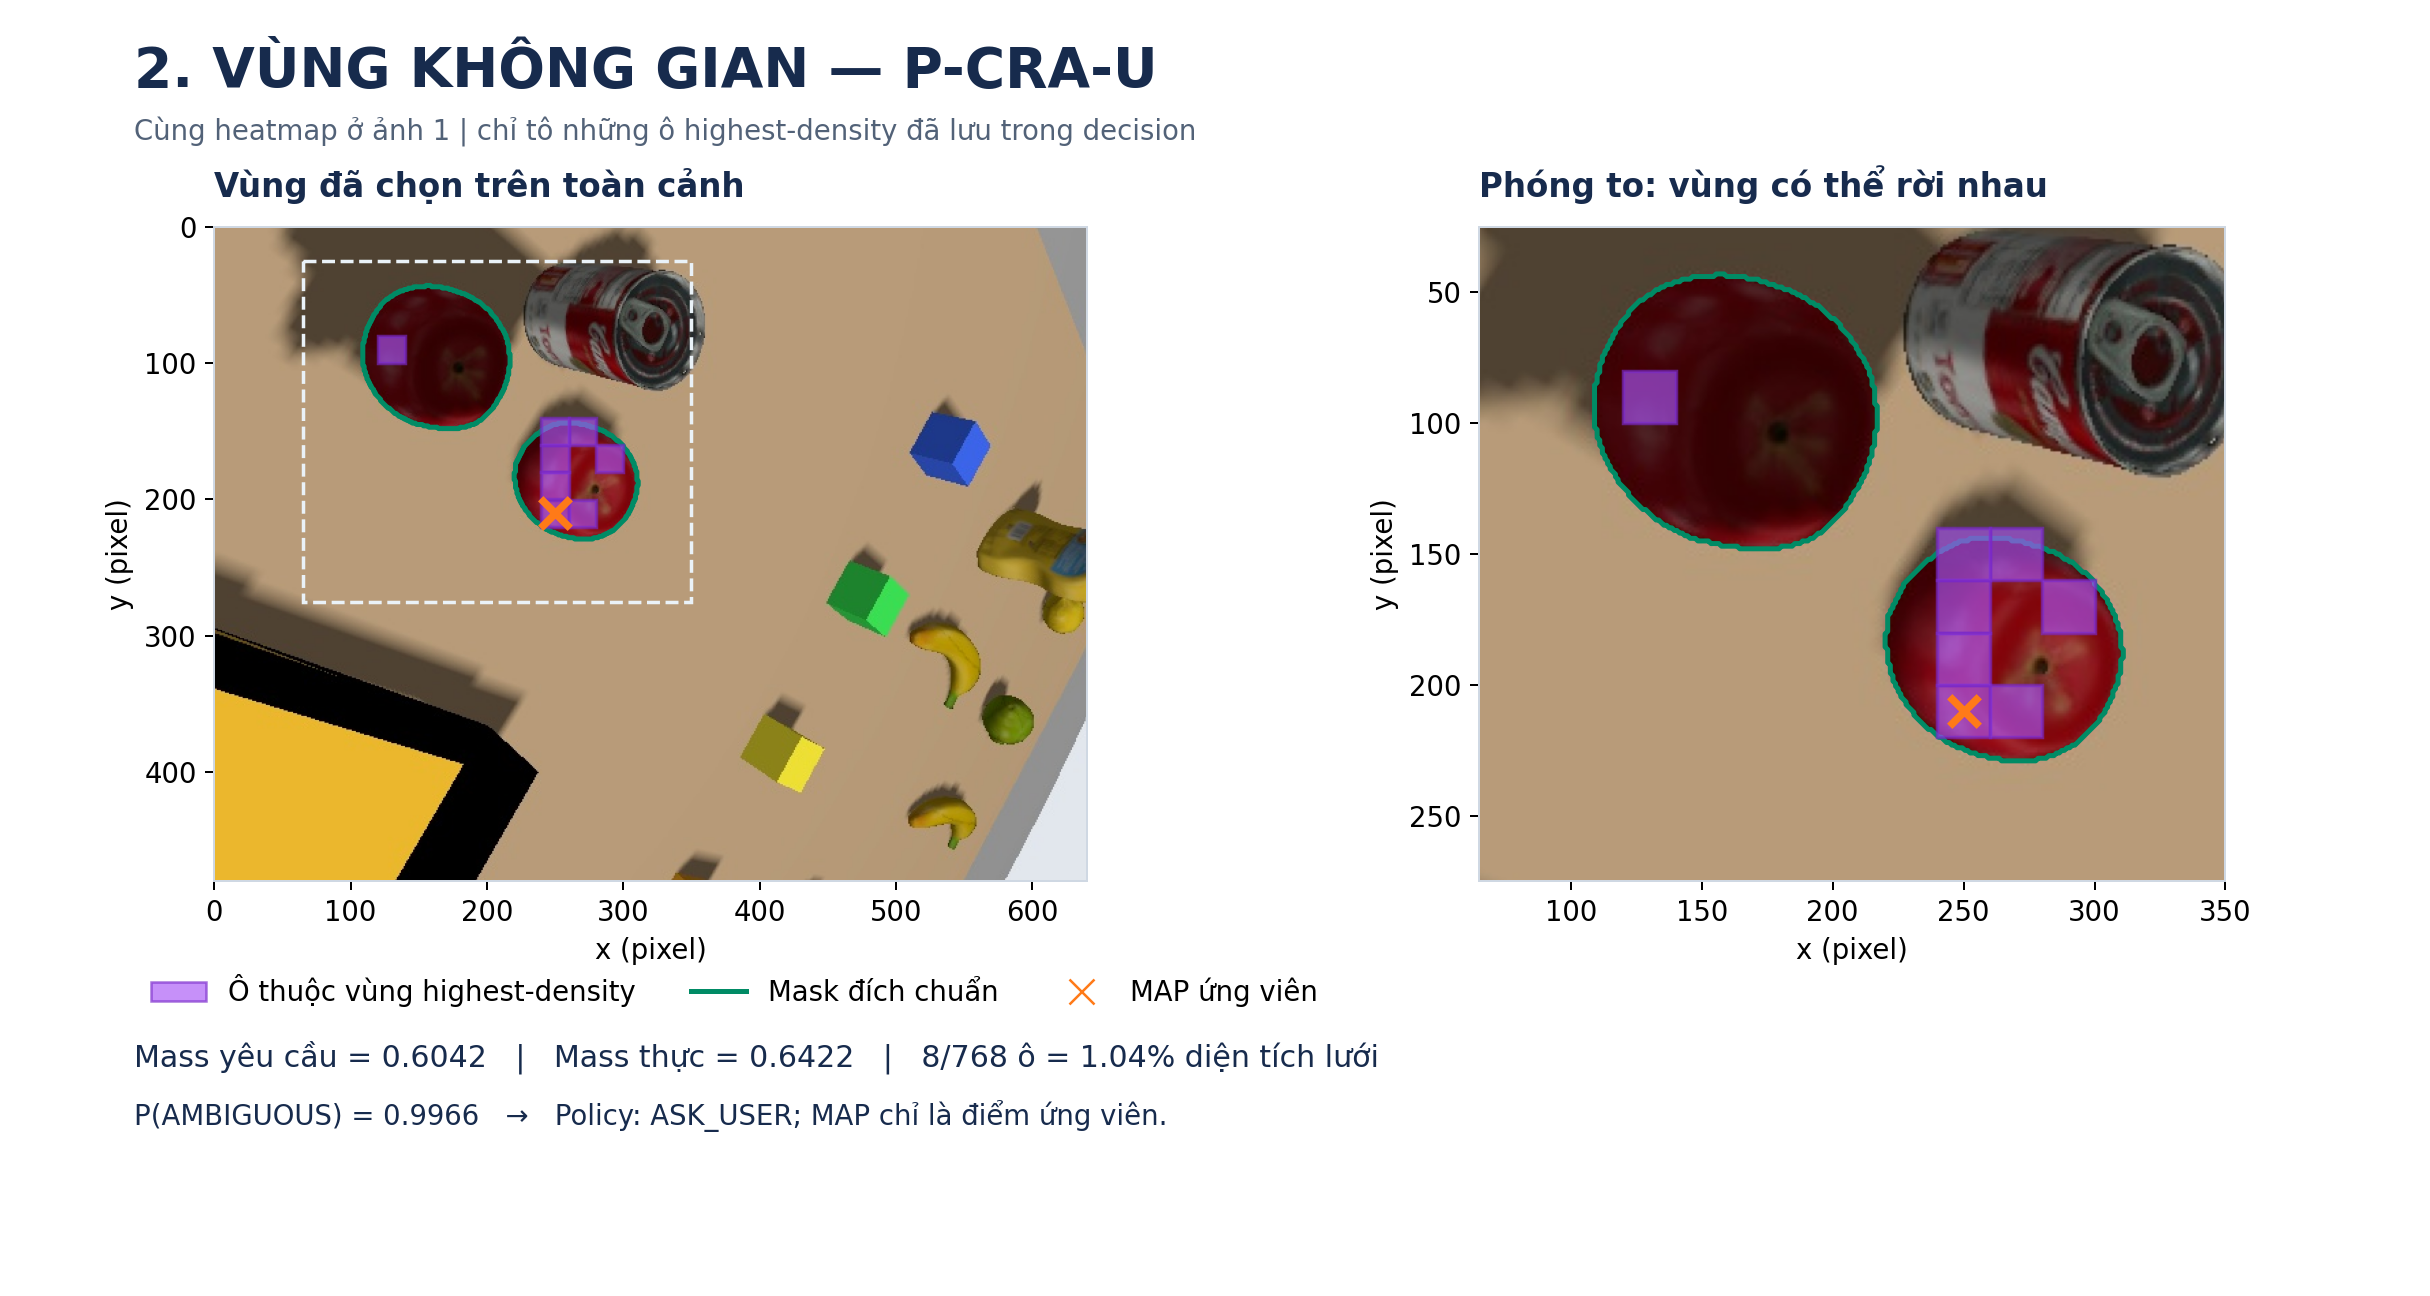
\includegraphics[width=\textwidth,height=0.66\textheight,keepaspectratio]{hinhanh/02_vung_khong_gian.png}
    \caption{Vùng highest-density đã lưu cho sample
    \texttt{v211iid\_\allowbreak family\_\allowbreak 000137\_\allowbreak \_\allowbreak clean}: mass yêu cầu
    0.6042, mass thực 0.6422 trên 8/768 ô lưới. Mẫu được
    dự đoán AMBIGUOUS nên policy chọn ASK\_USER; MAP và vùng
    xác suất không đồng nghĩa đã chọn đúng một vật duy nhất.}
    \label{fig:results-demo-spatial-region}
\end{figure}

Family dependence và sai khác giao thức
giới hạn việc viện dẫn bảo đảm conformal
hữu hạn mẫu. Kết quả ở đây là kiểm tra
empirical của vùng đã fit, không khẳng định
phân phối bất kỳ hoặc robot vật lý.

\begin{figure}[htbp]
    \centering
    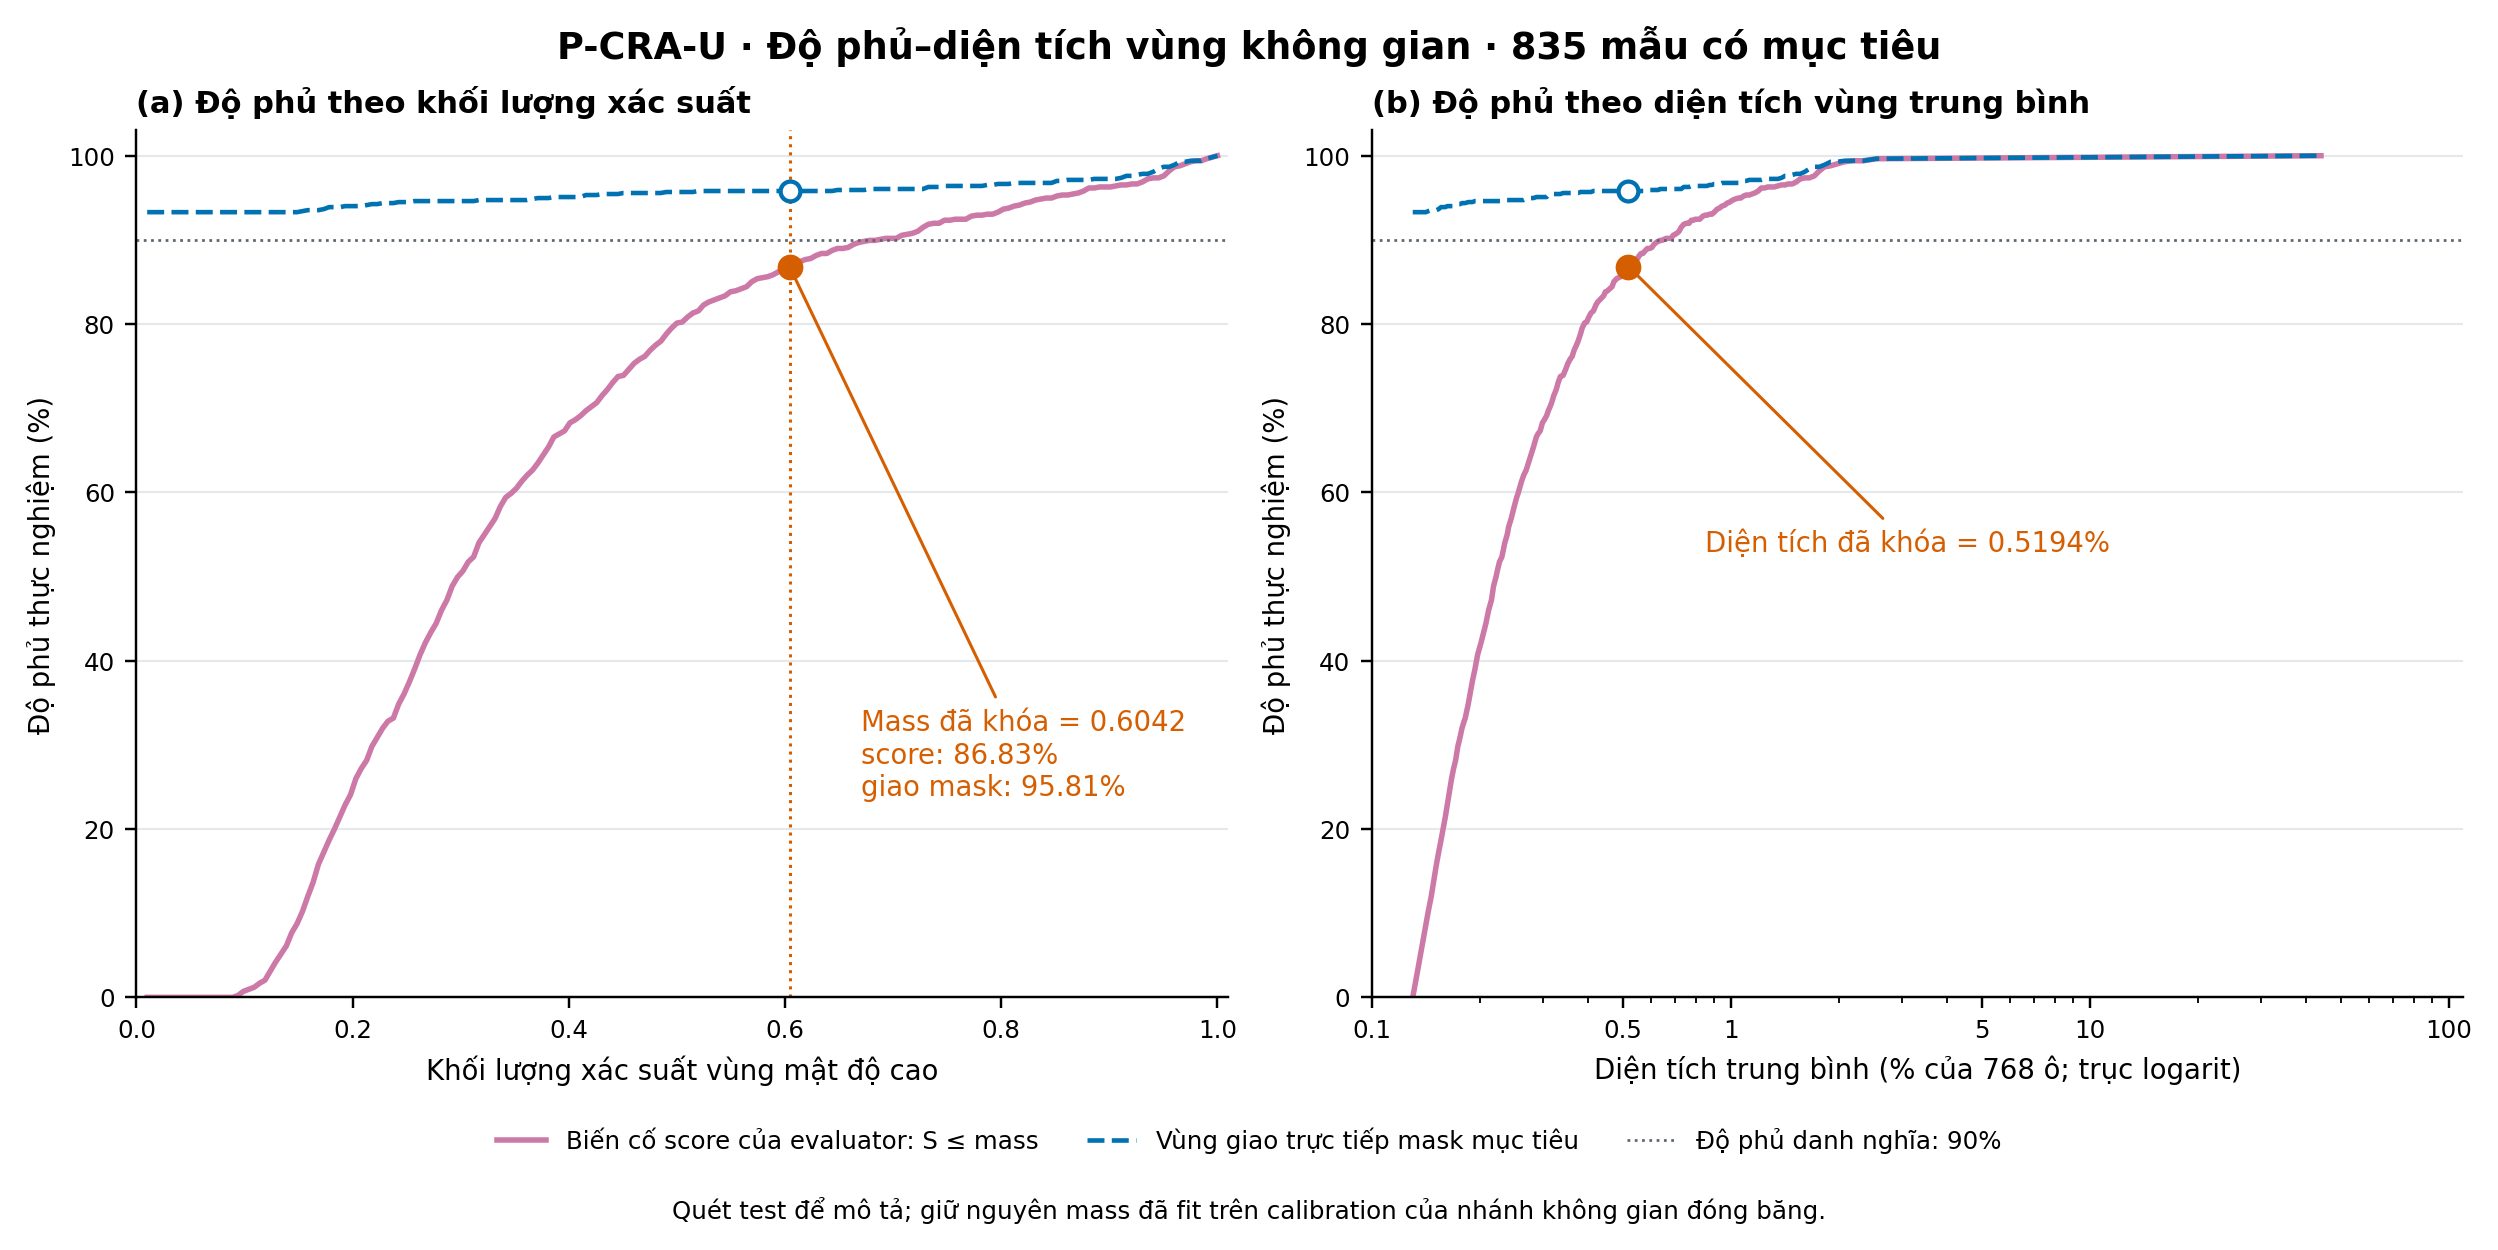
\includegraphics[width=\textwidth,height=0.60\textheight,keepaspectratio]{hinhanh/fig23_pcrau_coverage_area_adapter_vi.png}
    \caption{Coverage--area của vùng highest-density
    P-CRA-U trên 835 sample có target: (a) coverage
    theo mass yêu cầu; (b) coverage theo diện tích
    lưới trung bình, với trục diện tích logarithmic.
    Hai đường phân biệt score event $S_i\leq m$
    của evaluator với giao region--mask trực tiếp.
    Điểm mass đã khóa $m=0.6041832$ có diện tích
    trung bình 0.5194\%, score coverage 86.83\%
    và direct-intersection coverage 95.81\%.
    Đường ngang 90\% là nominal, không phải bảo đảm
    cho đường cong test.}
    \label{fig:results-coverage-area-pending}
    {\footnotesize Nguồn: probability grid và
    \texttt{target\_\allowbreak required\_\allowbreak hd\_\allowbreak mass} đã lưu, mask
    evaluator và region trong \texttt{decisions.jsonl};
    quét 201 giá trị mass bằng Matplotlib/NumPy,
    không chọn lại mass theo test.\par}
\end{figure}

Khi mass tăng, vùng nhận thêm ô nên diện tích và
coverage không giảm. Direct-intersection coverage
ở mass đã khóa là $800/835=95.81\%$, khác với
$725/835=86.83\%$ của score event trong
Bảng~\ref{tab:results-region}. Vùng hiển thị nhận
cả ô làm khối lượng tích lũy đạt hoặc vượt mass;
score event lại yêu cầu khối lượng đến ô target
đầu tiên không vượt mass. Vì vậy, một target nằm
ở ô vượt biên có thể giao vùng nhưng không đạt
score event. Ngoài ra, sáu sample có thứ tự ô
đồng xác suất khác giữa thao tác sắp xếp của
evaluator và policy; đường score giữ nguyên
giá trị đã lưu, đường giao vùng giữ đúng cách
hậu xử lý của policy.

Phân tích bổ sung này không thay định nghĩa hay
số liệu coverage đã báo của evaluator. Direct
intersection chỉ yêu cầu vùng chạm ít nhất một
pixel mask, không bảo đảm chứa toàn bộ vật hoặc
đủ chính xác cho thao tác. Đường cong là mô tả
từ prediction đã khóa, chưa có CI theo family
và không được dùng chọn lại mass cho P-CRA-U.

\section{Ablation và các experiment phát triển}
\label{sec:results-ablation}

\subsection{Trạng thái bằng chứng ablation}

So sánh RoboRefer--sidecar V2 thay đổi toàn đường
dự đoán, không phải ablation một thành phần.
Bảng~\ref{tab:results-ablation} giữ một hàng
V2 lịch sử và Adapter có số liệu, đồng thời chỉ rõ các hàng còn thiếu. Adapter là bước phát triển answerability; phép so sánh này không phải ablation riêng depth, relation hoặc ranking loss. Không suy ra đóng góp riêng của depth,
relation, anchor, source hay ranking loss
bằng cách điền lại số full model.

\begin{table}[htbp]
    \centering
    \setlength{\tabcolsep}{4pt}
    \renewcommand{\arraystretch}{1.15}
    \caption{Ma trận ablation trong phạm vi Test-IID.
    Hai phiên bản đầy đủ có kết quả; các nhánh bỏ thành phần chưa đánh giá.}
    \label{tab:results-ablation}
    \small
    \begin{tabularx}{\textwidth}{@{}>{\raggedright\arraybackslash}Xrrrr@{}}
        \toprule
        Cấu hình & \shortstack{PIT (\%)\\$\uparrow$} & \shortstack{Answer F1\\$\uparrow$} & \shortstack{Risk AP\\$\uparrow$} & \shortstack{Brier\\$\downarrow$} \\
        \midrule
        V2 lịch sử & 92.81 & 0.7752 & 0.9620 & 0.09615 \\
        P-CRA-U (Adapter) & 92.81 & 0.8097 & 0.9674 & 0.07711 \\
        Bỏ depth, retrain tương ứng & -- & -- & -- & -- \\
        Bỏ relation slots & -- & -- & -- & -- \\
        Bỏ anchor head & -- & -- & -- & -- \\
        Bỏ source supervision & -- & -- & -- & -- \\
        Bỏ counterfactual ranking & -- & -- & -- & -- \\
        Scalar-only calibration & -- & -- & -- & -- \\
        \bottomrule
    \end{tabularx}
    \vspace{2pt}
    {\footnotesize\raggedright Nguồn: full V2 Test-IID; các đối chứng
    còn lại chưa có kết quả khóa cùng protocol.
    PIT dùng 835 mẫu, các cột còn lại dùng 1000 mẫu.\par}
\end{table}

Test-time tắt depth của một model đã học
RGB-D là stress test thiếu phương thức,
không tương đương RGB-only được retrain.
Bỏ source khỏi vector nhưng giữ hệ số
logistic cũ cũng không phải đối chứng
scalar-only hợp lệ. Các hạn chế này khiến
RQ1 và RQ4 chưa được trả lời ở mức cô lập
đóng góp kiến trúc.

\subsection{Diễn biến huấn luyện V2}

\begin{table}[htbp]
    \centering
    \setlength{\tabcolsep}{4pt}
    \renewcommand{\arraystretch}{1.15}
    \caption{Một số mốc history V2. Epoch đánh số từ 0;
    checkpoint sử dụng là epoch 13, không phải cuối run.}
    \label{tab:results-v2-history}
    \small
    \begin{tabularx}{\textwidth}{@{}>{\raggedright\arraybackslash}Xrrrr@{}}
        \toprule
        Epoch & \shortstack{Train total\\$\downarrow$} & \shortstack{Dev total\\$\downarrow$} & \shortstack{Dev PIT (\%)\\$\uparrow$} & \shortstack{LR cuối\\epoch} \\
        \midrule
        0 & 4.83731 & 3.65689 & 42.69 & $8.10\times10^{-5}$ \\
        5 & 2.19667 & 2.13034 & 85.97 & $1.80902\times10^{-4}$ \\
        13 & 1.17249 & 1.69711 & 97.31 & $5.26131\times10^{-5}$ \\
        19 & 0.94789 & 1.79097 & 97.31 & 0 \\
        \bottomrule
    \end{tabularx}
    \vspace{2pt}
    {\footnotesize\raggedright Nguồn: history của
    \texttt{pcrau\_\allowbreak target\_\allowbreak v2\_\allowbreak full\_\allowbreak seed\_\allowbreak 24082026}.
    PIT dev dùng 335 sample có target.\par}
\end{table}

Train loss tiếp tục giảm sau epoch 13
nhưng dev total tăng ở cuối run. Diễn biến
này phù hợp với dấu hiệu overfit theo
tiêu chí dev loss; grounding tổng có thể
không đổi do không phản ánh toàn bộ nhiệm
vụ đa head. Best được chọn bằng dev total,
không chọn lại bằng Test-IID.

\subsection{Diễn biến huấn luyện Adapter}

Adapter có 25 bản ghi epoch 0--24. Hình mới dùng loss train Adapter
và accuracy/macro-F1 answerability dev; log không lưu loss dev theo
epoch, nên không vẽ đường dev loss giả định. Best epoch 13/step 1120
được chọn bằng macro-F1 dev trong các checkpoint qua cổng, khác tiêu
chí dev total loss của V2. Best đạt macro-F1 dev 0.8725; mức Test-IID
0.8097 cho thấy cải thiện dev không chuyển nguyên vẹn sang test.

\begin{figure}[htbp]
    \centering
    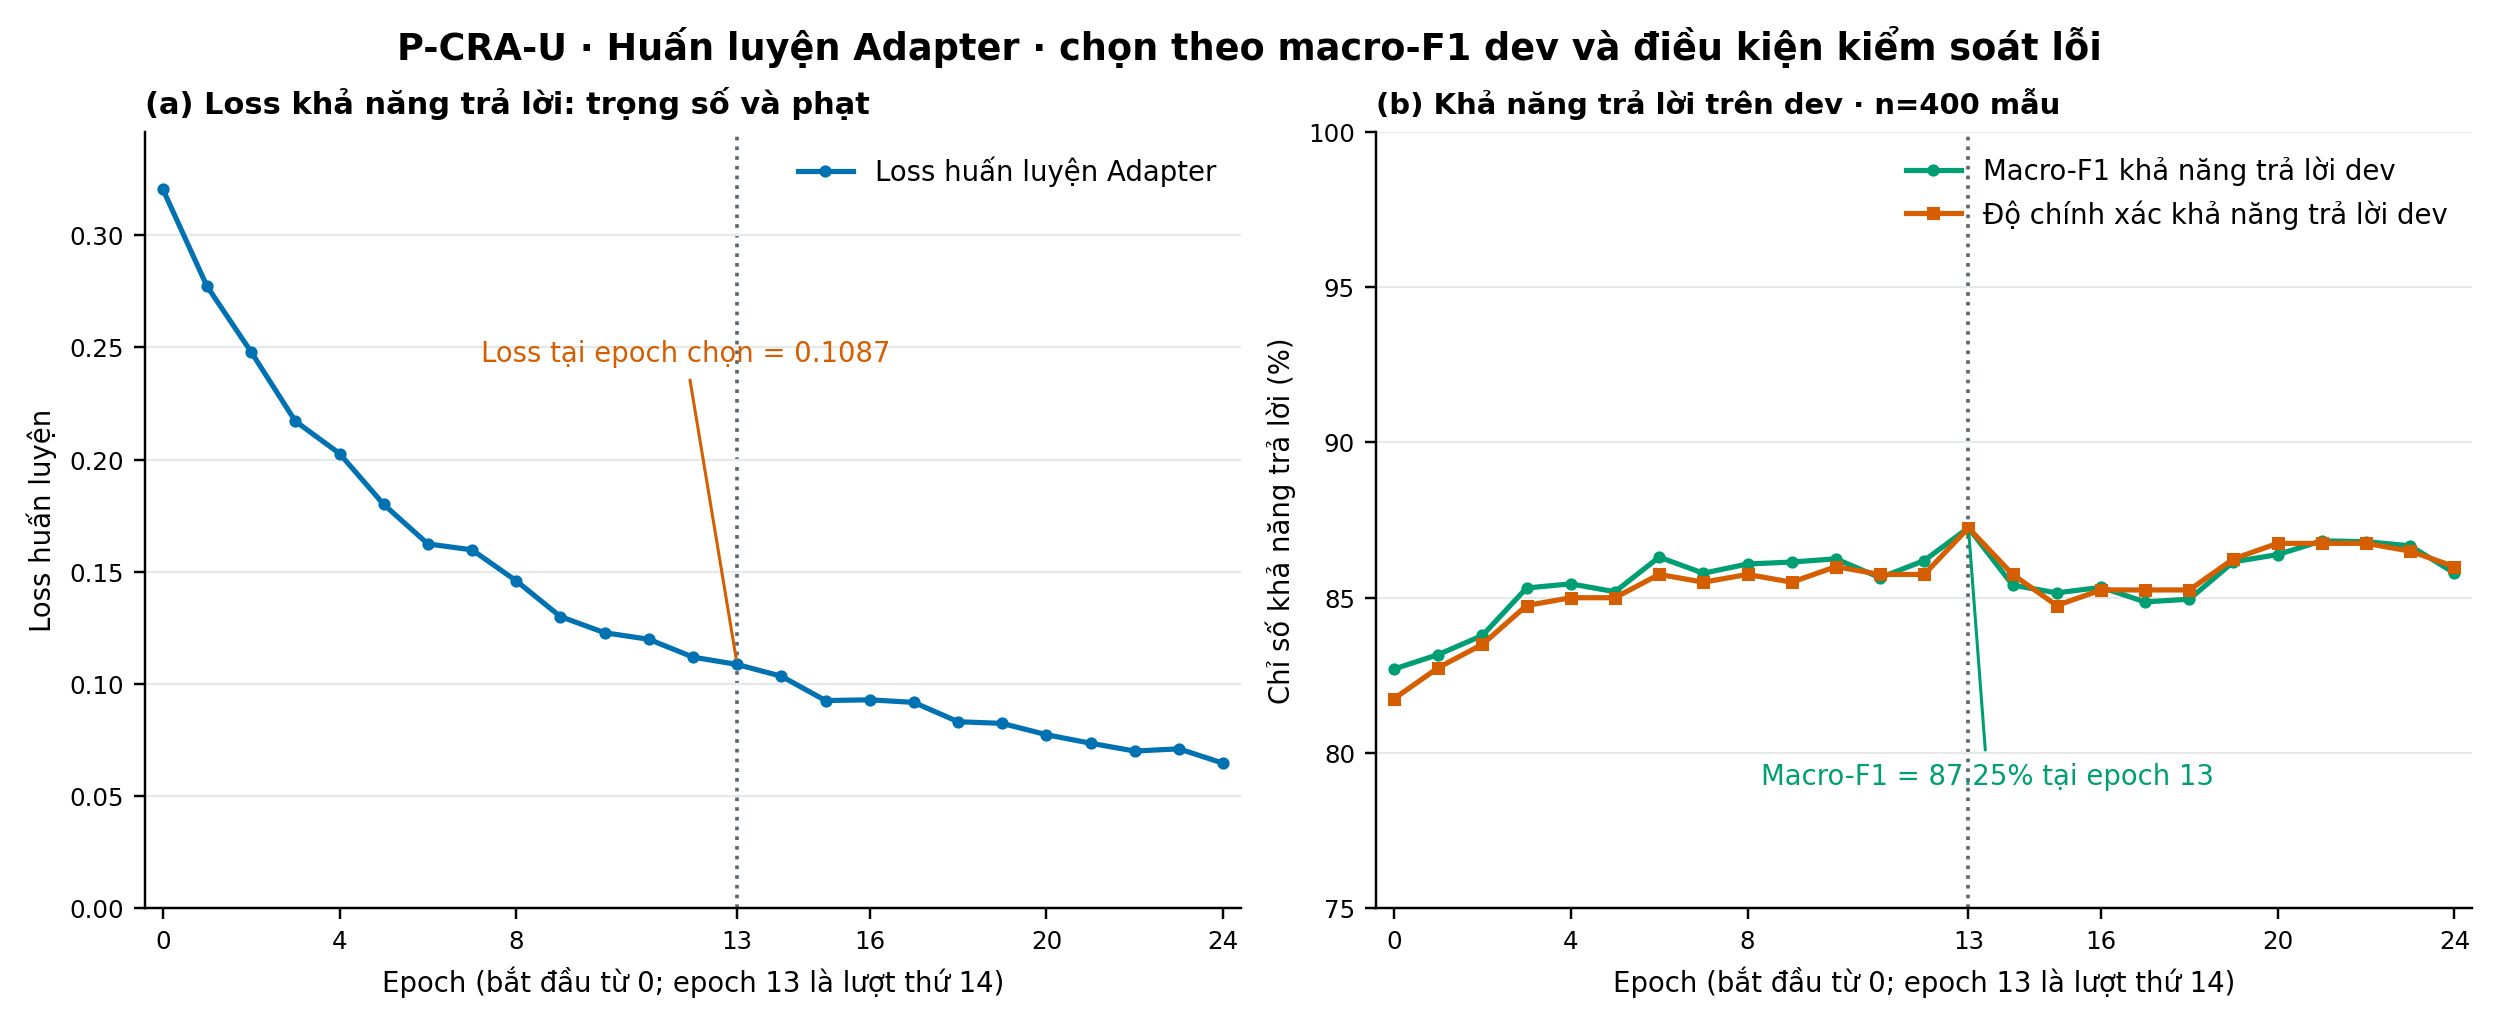
\includegraphics[width=\textwidth,height=0.55\textheight,keepaspectratio]{hinhanh/fig20_pcrau_training_curves_adapter_vi.png}
    \caption{Huấn luyện Adapter P-CRA-U: (a) loss train Adapter;
    (b) accuracy và macro-F1 answerability trên 400 mẫu dev.
    Đường dọc đánh dấu best epoch 13/step 1120, chọn bằng macro-F1
    dev và các cổng phân loại. Epoch đánh số từ 0.}
    \label{fig:results-training-pending}
    {\footnotesize Nguồn: \texttt{detail\_\allowbreak cost/history.jsonl} và
    metadata best Adapter; không ghép loss Adapter với loss đa nhiệm V2.\par}
\end{figure}

\subsection{V3 regularized với ba seed}

V3 đồng thời đổi dropout, modality dropout,
weight decay, learning rate, sampling và
source penalty. Đây là experiment phát
triển gộp nhiều thay đổi, không phải
ablation cô lập. Ba run có history nhưng
không seed nào vượt cổng dev grounding
0.97 để tạo best checkpoint đủ điều kiện.

\begin{table}[htbp]
    \centering
    \setlength{\tabcolsep}{4pt}
    \renewcommand{\arraystretch}{1.15}
    \caption{Grounding dev lớn nhất trong history của ba seed V3.}
    \label{tab:results-v3-seeds}
    \small
    \begin{tabularx}{\textwidth}{@{}rrrr>{\raggedright\arraybackslash}X@{}}
        \toprule
        Seed & \shortstack{Số epoch\\ghi} & \shortstack{Epoch\\cực đại} & \shortstack{Max dev\\PIT (\%)} & \shortstack{Best đủ\\cổng 97\%} \\
        \midrule
        24082026 & 20 & 16 & 91.04 & Không \\
        24082027 & 20 & 16 & 88.36 & Không \\
        24082028 & 20 & 16 & 89.85 & Không \\
        \bottomrule
    \end{tabularx}
    \vspace{2pt}
    {\footnotesize\raggedright Nguồn: history từng run V3 và trạng thái
    experiment; max trên history không phải một checkpoint
    đã được khóa cho đánh giá chính thức.\par}
\end{table}

Việc tăng regularization không tự bảo đảm
cải thiện. Với ba seed này, mục tiêu giữ
grounding dev ít nhất 97\% chưa đạt, nên
V2 được giữ làm nền đóng băng cho Adapter hiện tại.
Không báo mean/std Test-IID V3 khi chưa
có ba checkpoint và artifact đánh giá
hợp lệ. Các run này cũng không tạo ra
bằng chứng ba seed độc lập cho hiệu quả
của V2, vì V2 chính chỉ có một seed.

\section{Phân tích Test-IID theo nhóm dữ liệu}
\label{sec:results-iid}

\subsection{Đối chiếu dev, calibration và test}

Test-IID được capture mới, không lấy 80 family dev
đổi tên thành test. Các tập giữ vai trò riêng khi tối ưu; riêng IID cũ đã từng được phân tích trước vòng phát triển Adapter.
Cùng registry asset và template giữ phạm vi IID
của giao thức, không bảo đảm mọi thành phần phân
bố hoàn toàn giống nhau. Quota ưu tiên hoa quả
và camera khóa không loại bỏ khác biệt layout.

\begin{table}[htbp]
    \centering
    \setlength{\tabcolsep}{4pt}
    \renewcommand{\arraystretch}{1.15}
    \caption{P-CRA-U có Adapter trên các split.
    Dev chọn Adapter, calibration fit hậu xử lý; Test-IID là đánh giá lại.}
    \label{tab:results-split-comparison}
    \small
    \begin{tabularx}{\textwidth}{@{}>{\raggedright\arraybackslash}Xrrrrr@{}}
        \toprule
        Tập & \shortstack{Family /\\sample} & \shortstack{Target-\\present} & \shortstack{PIT\\(\%)} & \shortstack{Answer\\macro-F1} & \shortstack{Source\\macro-F1} \\
        \midrule
        Dev & 80 / 400 & 335 & 97.31 & 0.8725 & 0.6664 \\
        Calibration & 200 / 1000 & 835 & 97.25 & 0.8434 & 0.6807 \\
        Test-IID & 200 / 1000 & 835 & 92.81 & 0.8097 & 0.6774 \\
        \bottomrule
    \end{tabularx}
    \vspace{2pt}
    {\footnotesize\raggedright Nguồn: evaluation của run V2 và Test-IID.
    Dev/calibration không phải hai bộ test độc lập;
    PIT dùng mẫu có mask, F1 dùng toàn bộ sample mỗi tập.\par}
\end{table}

Grounding test giảm so với dev/calibration trong
khi source macro-F1 gần calibration. Các head
không nhất thiết suy giảm cùng mức. Không chọn
lại V2 theo bảng này; các nhóm test yếu là
hạn chế của mô hình đã khóa.

\subsection{Phân tầng theo nhóm vật đích}

Bảng~\ref{tab:results-object-strata} dùng nhóm
target chính của family, chỉ lấy variant có
mask. Số family cho biết quy mô cluster; $n$
là sample đủ điều kiện, không phải ảnh độc lập.

\begin{table}[htbp]
    \centering
    \setlength{\tabcolsep}{4pt}
    \renewcommand{\arraystretch}{1.15}
    \caption{Grounding theo nhóm vật đích.
    CI 95\% của chênh lệch dùng cluster bootstrap paired.}
    \label{tab:results-object-strata}
    \small
    \begin{tabularx}{\textwidth}{@{}>{\raggedright\arraybackslash}Xrrrrr@{}}
        \toprule
        Nhóm & Family & $n$ & \shortstack{RoboRefer\\(\%)} & \shortstack{P-CRA-U\\(\%)} & \shortstack{$\Delta$ pp\\{[CI 95\%]}} \\
        \midrule
        Hoa quả & 110 & 478 & 79.08 & 95.40 & $+16.32\ [10.57,22.18]$ \\
        Cốc & 30 & 112 & 97.32 & 96.43 & $-0.89\ [-6.87,5.15]$ \\
        Hộp & 20 & 91 & 96.70 & 67.03 & $-29.67\ [-41.58,-17.57]$ \\
        Chai/lon & 30 & 122 & 97.54 & 99.18 & $+1.64\ [-1.50,4.94]$ \\
        Cube & 10 & 32 & 93.75 & 90.62 & $-3.12\ [-25.00,16.67]$ \\
        \midrule
        Tổng & 200 & 835 & 86.71 & 92.81 & $+6.11\ [1.78,10.49]$ \\
        \bottomrule
    \end{tabularx}
    \vspace{2pt}
    {\footnotesize\raggedright Nguồn: \texttt{target\_\allowbreak object\_\allowbreak group}
    của \texttt{full\_\allowbreak comparison.json}; chai/lon tương ứng
    \texttt{container}. CI dùng 20000 lượt, seed từng
    phân tầng lưu trong artifact.\par}
\end{table}

Hoa quả tăng từ 378/478 lên 456/478,
thêm 78 hit, đóng góp lớn vào mức tăng
chung. Ngược lại, hộp giảm từ 88/91
xuống 61/91, mất 27 hit, với CI hoàn
toàn âm. V2 không tốt hơn RoboRefer
trên mọi nhóm.

Nhóm hộp có 30 RoboRefer-only và chỉ
3 V2-only; hồi quy không phải một ảnh
đơn lẻ. Chưa có kiểm tra cô lập để
quy lỗi cho kích thước, texture hay
depth; đó là giả thuyết cần nghiên
cứu. Cube chỉ có 10 family và CI
rộng, chưa đủ kết luận ưu thế.

Hồi quy nhóm hộp là giới hạn thực nghiệm đáng kể của phương pháp,
không được che bởi accuracy tổng. Kết quả tổng thể còn phụ thuộc tỷ trọng
nhóm vật của Test-IID; chưa có cơ sở suy ra mức tăng $+6.11$ pp giữ nguyên
khi thay phân bố vật thể. Các case hồi quy giúp nhận diện lỗi để nghiên
cứu tiếp, nhưng chưa cô lập nguyên nhân do feature, fusion hay supervision.

\begin{figure}[htbp]
    \centering
    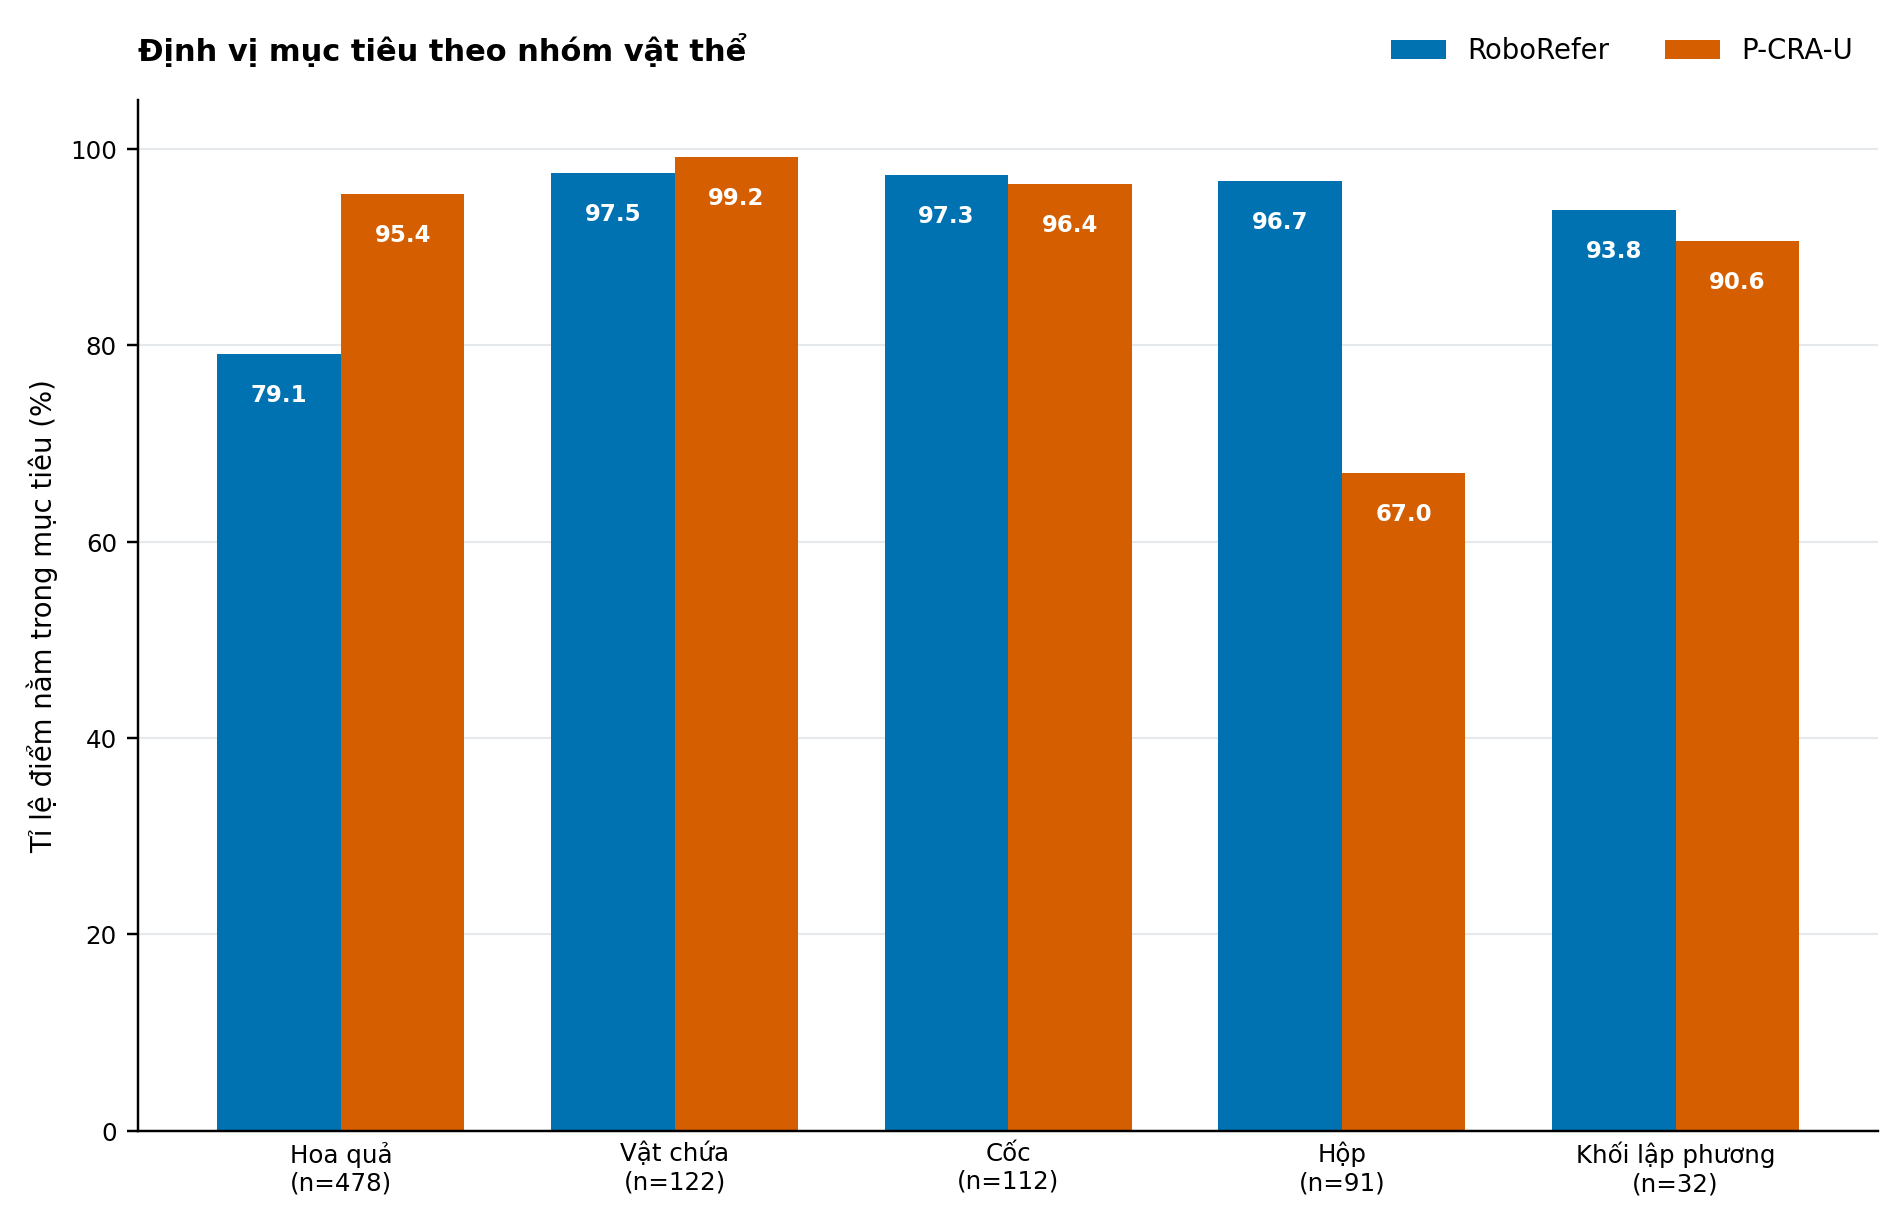
\includegraphics[width=\textwidth,height=0.58\textheight,keepaspectratio]{hinhanh/fig16_grounding_by_object_adapter_vi.png}
    \caption{Grounding theo nhóm vật đích.
    Biểu đồ không vẽ error bar; CI đầy đủ được giữ
    ở Bảng~\ref{tab:results-object-strata}.}
    \label{fig:results-object-strata}
    {\footnotesize Nguồn: prediction paired và
    evaluator Test-IID; cột dùng thang phần trăm.\par}
\end{figure}

\subsection{Phân tầng theo quan hệ vận hành}

\begin{table}[htbp]
    \centering
    \setlength{\tabcolsep}{4pt}
    \renewcommand{\arraystretch}{1.15}
    \caption{Point-in-target theo relation audit.
    Đây không phải relation classification accuracy.}
    \label{tab:results-relation-strata}
    \small
    \begin{tabularx}{\textwidth}{@{}>{\raggedright\arraybackslash}Xrrrrr@{}}
        \toprule
        Quan hệ & Family & $n$ & \shortstack{RoboRefer\\(\%)} & \shortstack{P-CRA-U\\(\%)} & \shortstack{$\Delta$ pp\\{[CI 95\%]}} \\
        \midrule
        \texttt{direct} & 200 & 338 & 92.01 & 90.83 & $-1.18\ [-7.43,5.23]$ \\
        \texttt{left\_\allowbreak of} & 29 & 53 & 96.23 & 88.68 & $-7.55\ [-17.74,0.00]$ \\
        \texttt{right\_\allowbreak of} & 27 & 57 & 75.44 & 94.74 & $+19.30\ [-1.72,40.91]$ \\
        \texttt{front\_\allowbreak of} & 53 & 137 & 83.94 & 94.89 & $+10.95\ [0.00,22.50]$ \\
        \texttt{behind} & 56 & 78 & 89.74 & 98.72 & $+8.97\ [0.90,19.23]$ \\
        \texttt{nearer\_\allowbreak than} & 27 & 57 & 78.95 & 96.49 & $+17.54\ [3.77,33.33]$ \\
        \texttt{farther\_\allowbreak than} & 26 & 46 & 76.09 & 95.65 & $+19.57\ [0.00,39.13]$ \\
        \texttt{between\_\allowbreak in\_\allowbreak depth} & 10 & 30 & 90.00 & 76.67 & $-13.33\ [-39.39,9.09]$ \\
        \texttt{nearer\_\allowbreak than\_\allowbreak both} & 13 & 39 & 69.23 & 97.44 & $+28.21\ [3.33,55.56]$ \\
        \bottomrule
    \end{tabularx}
    \vspace{2pt}
    {\footnotesize\raggedright Nguồn: phân tầng \texttt{relation},
    so sánh paired Test-IID. Một family có thể góp
    sample vào nhiều hàng; không cộng số family.
    CI chưa hiệu chỉnh multiple comparisons.\par}
\end{table}

Nearer, behind và nearer-than-both có
ước lượng dương và CI không chứa 0.
Nhưng phân tầng nhỏ và nhiều so sánh
đòi hỏi thận trọng; chưa hiệu chỉnh
việc lựa chọn nhiều nhóm.

Left-of và between-in-depth có ước
lượng thấp hơn baseline. Between
chỉ có 10 family, CI rộng; cần thêm
cảnh độc lập hoặc thí nghiệm kiểm
soát, không chỉ thêm câu lệnh từ
cùng ảnh rồi coi là bằng chứng mới.

\begin{figure}[htbp]
    \centering
    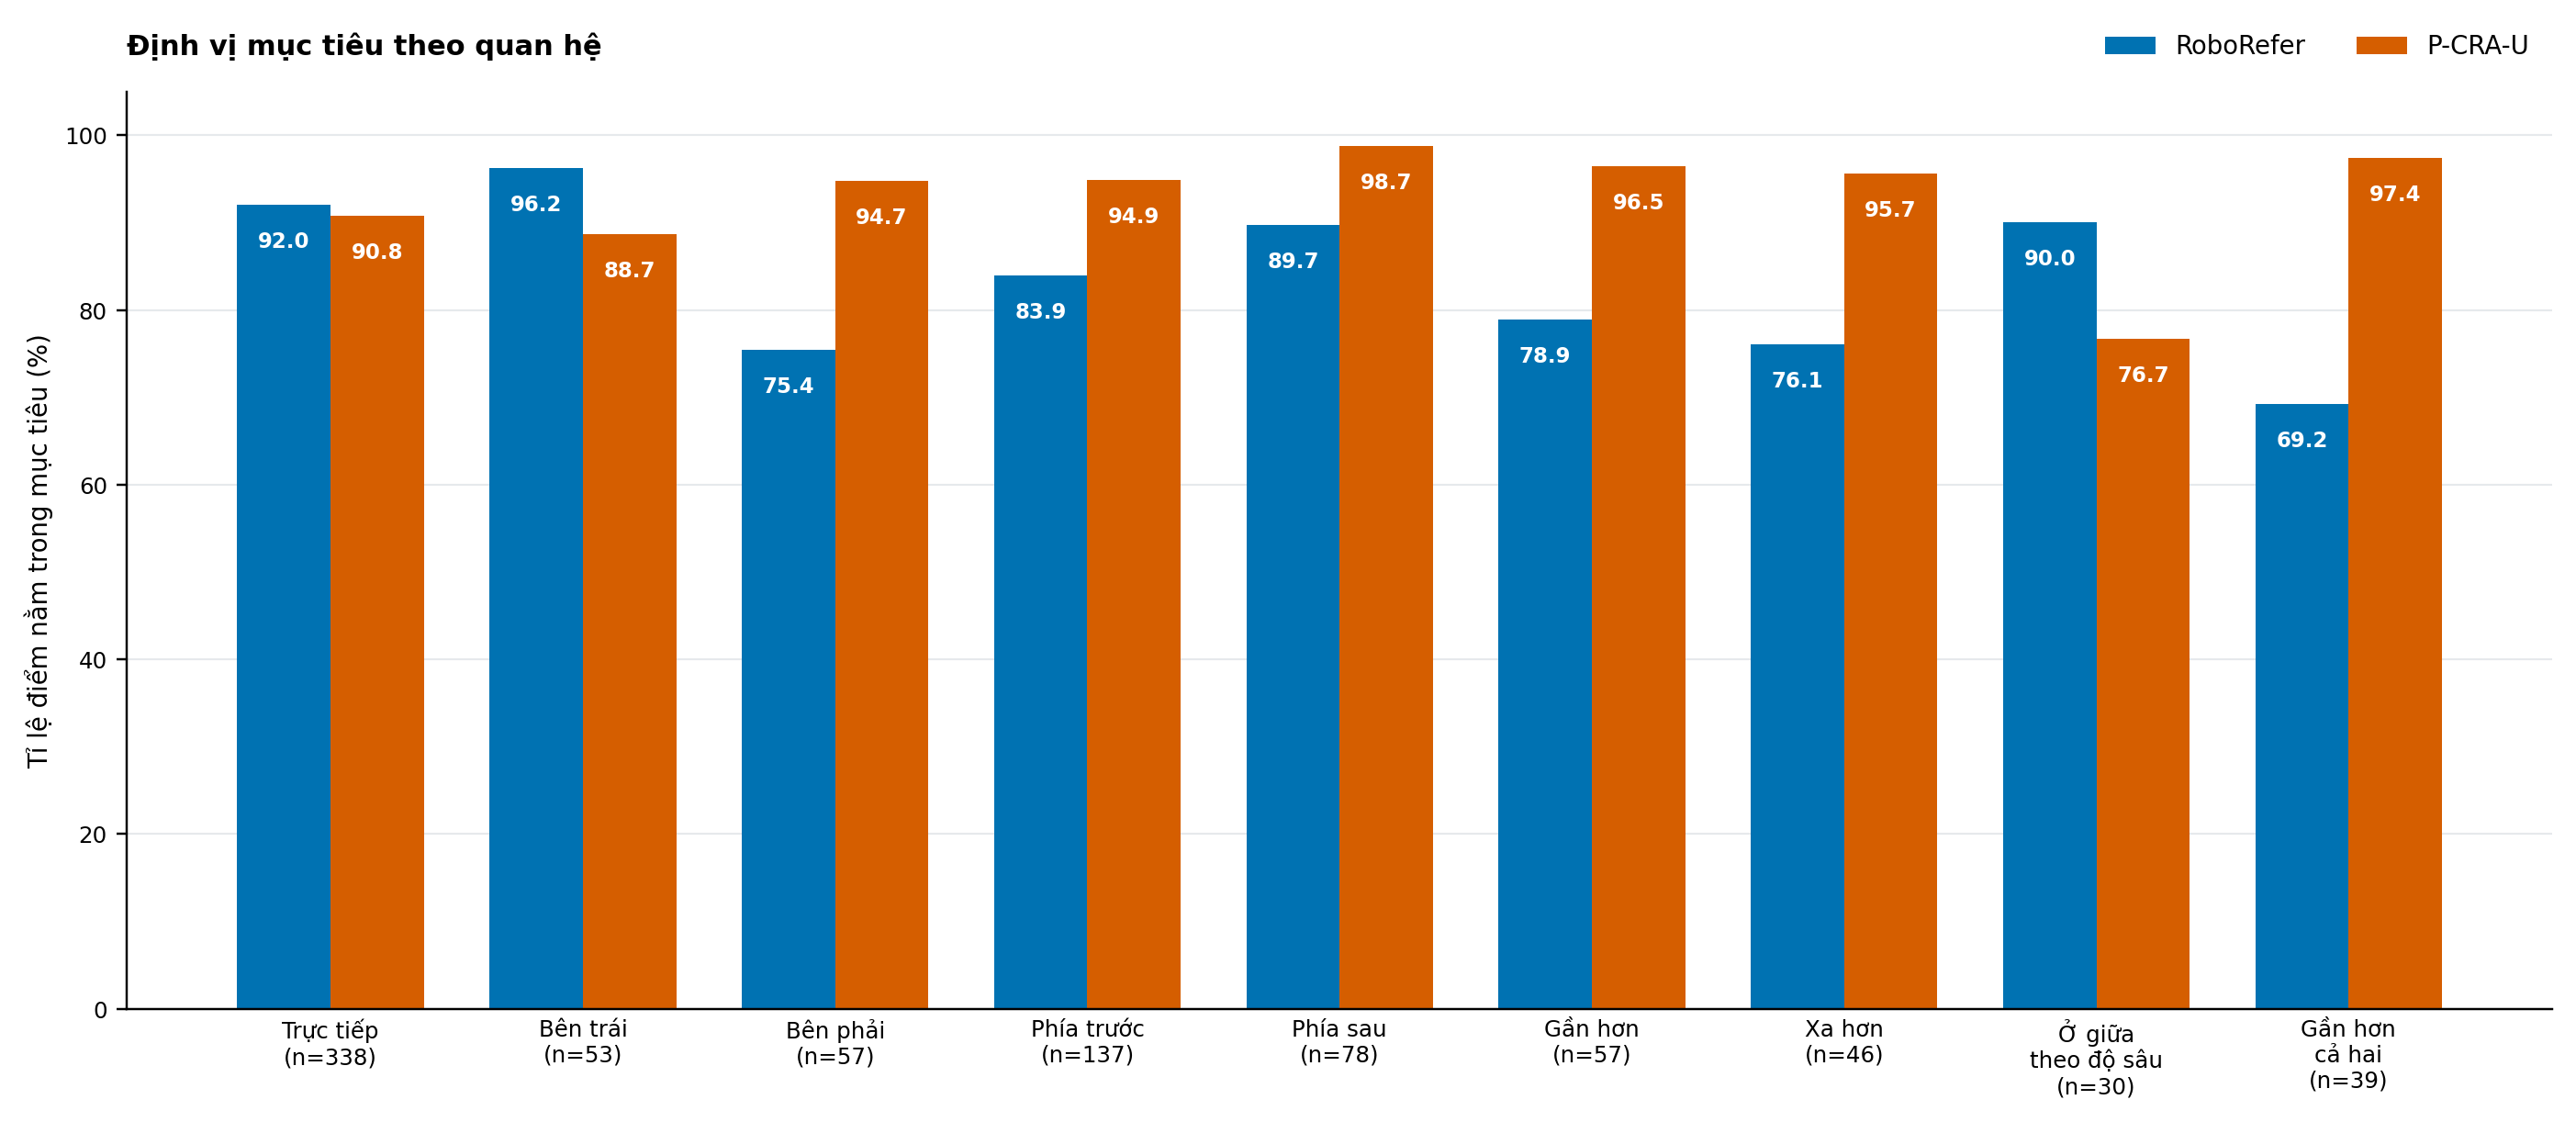
\includegraphics[width=\textwidth,height=0.60\textheight,keepaspectratio]{hinhanh/fig17_grounding_by_relation_adapter_vi.png}
    \caption{Grounding theo relation audit.
    CI không vẽ trên cột và được báo ở
    Bảng~\ref{tab:results-relation-strata}.}
    \label{fig:results-relation-strata}
    {\footnotesize Nguồn: so sánh paired trên
    sample có target của Test-IID.\par}
\end{figure}

\subsection{Phân tầng theo counterfactual}

\begin{table}[htbp]
    \centering
    \setlength{\tabcolsep}{4pt}
    \renewcommand{\arraystretch}{1.15}
    \caption{Grounding theo năm variant.
    $n$ chỉ gồm sample có target; mỗi variant có tổng 200 sample.}
    \label{tab:results-variant-strata}
    \small
    \begin{tabularx}{\textwidth}{@{}>{\raggedright\arraybackslash}Xrrrr@{}}
        \toprule
        Variant & $n$ & \shortstack{RoboRefer\\(\%)} & \shortstack{P-CRA-U\\(\%)} & \shortstack{$\Delta$ pp\\{[CI 95\%]}} \\
        \midrule
        Clean & 154 & 83.12 & 90.91 & $+7.79\ [0.00,15.54]$ \\
        Semantic CF & 200 & 96.00 & 99.50 & $+3.50\ [1.00,6.50]$ \\
        Relation CF & 173 & 89.60 & 94.80 & $+5.20\ [-0.56,10.92]$ \\
        Depth corruption & 154 & 81.17 & 88.31 & $+7.14\ [-1.33,15.75]$ \\
        Occlusion/view CF & 154 & 80.52 & 88.31 & $+7.79\ [-0.64,16.20]$ \\
        \bottomrule
    \end{tabularx}
    \vspace{2pt}
    {\footnotesize\raggedright Nguồn: phân tầng \texttt{variant},
    bootstrap theo family. Clean không mặc định FOUND.\par}
\end{table}

Ước lượng tăng ở cả năm variant,
nhưng CI depth, occlusion và relation
chứa 0. Semantic CF đạt 199/200 hit
ở V2. Toàn bộ semantic CF của test
hiện tại có nhãn FOUND; điểm cao
không chứng minh phát hiện tốt
semantic absence.

\begin{figure}[htbp]
    \centering
    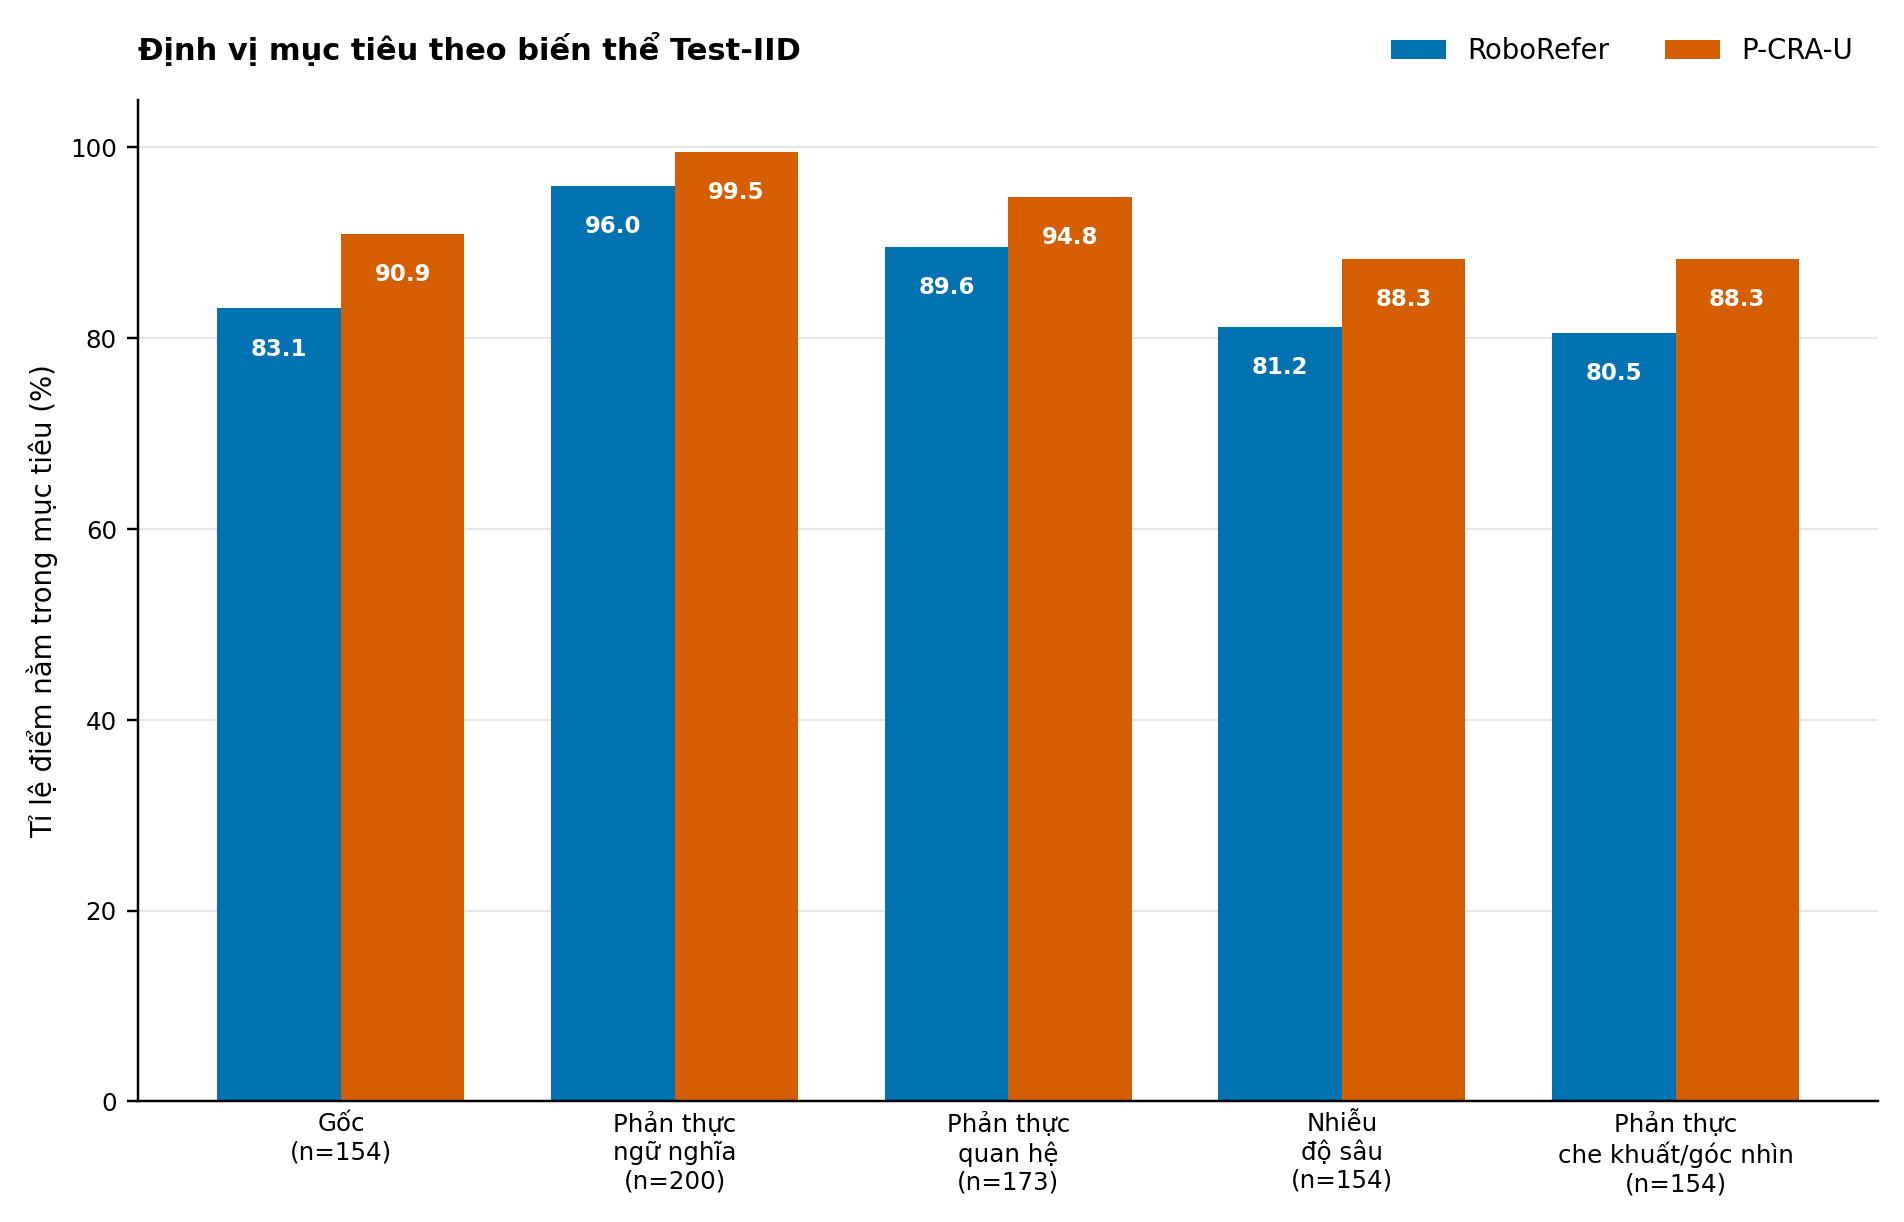
\includegraphics[width=\textwidth,height=0.58\textheight,keepaspectratio]{hinhanh/fig18_grounding_by_variant_adapter_vi.png}
    \caption{Grounding theo counterfactual.
    Tỉ lệ dùng sample có target, không mặc định
    mẫu số 200 cho mọi variant.}
    \label{fig:results-variant-strata}
    {\footnotesize Nguồn: paired prediction và
    evaluator; CI tại
    Bảng~\ref{tab:results-variant-strata}.\par}
\end{figure}

\begin{table}[htbp]
    \centering
    \setlength{\tabcolsep}{4pt}
    \renewcommand{\arraystretch}{1.15}
    \caption{Answerability, risk và policy theo variant,
    mỗi hàng dùng toàn bộ 200 sample.}
    \label{tab:results-variant-multitask}
    \small
    \begin{tabularx}{\textwidth}{@{}>{\raggedright\arraybackslash}Xrrrr@{}}
        \toprule
        Variant & \shortstack{Answer acc.\\(\%)} & \shortstack{Risk\\trung bình} & \shortstack{Tỉ lệ lỗi\\(\%)} & \shortstack{Policy acc.\\(\%)} \\
        \midrule
        Clean & 73.50 & 0.6969 & 63.50 & 67.00 \\
        Semantic CF & 98.00 & 0.0364 & 0.50 & 98.00 \\
        Relation CF & 74.50 & 0.3843 & 33.50 & 67.00 \\
        Depth corruption & 86.00 & 0.9750 & 100.00 & 86.00 \\
        Occlusion/view CF & 73.50 & 0.8031 & 100.00 & 76.50 \\
        \bottomrule
    \end{tabularx}
    \vspace{2pt}
    {\footnotesize\raggedright Nguồn: \texttt{strata.variant} trong
    \texttt{full\_\allowbreak metrics.json}. Lỗi là non-FOUND
    hoặc điểm ngoài target; policy acc. so intervention
    label, không phải recovery/task success.\par}
\end{table}

Depth và occlusion có tỉ lệ lỗi 100\%
theo tiêu chuẩn chấp nhận dù nhiều
điểm vẫn trúng mask. Không có mâu
thuẫn: thiếu bằng chứng vẫn phải
chặn. Mean risk depth 0.9750 cao
hơn occlusion 0.8031, phù hợp với
source depth dễ phân biệt hơn.

\section{Đánh giá quyết định chọn lọc}
\label{sec:results-selective}

\subsection{Phân bố bốn quyết định}

Policy Adapter cho 361 EXECUTE, 347 REOBSERVE, 134 ASK\_USER
và 158 ABSTAIN. Không execute chiếm 63.90\%, giảm từ 74.50\%
của V2. Đây là quyết định từ ảnh, chưa phải 639 lượt can thiệp thật.

\begin{table}[htbp]
    \centering
    \setlength{\tabcolsep}{4pt}
    \renewcommand{\arraystretch}{1.15}
    \caption{Bốn quyết định trên cùng 1000 mẫu Test-IID.}
    \label{tab:results-policy-counts}
    \small
    \begin{tabularx}{\textwidth}{@{}>{\raggedright\arraybackslash}Xrrr@{}}
        \toprule
        Quyết định & V2 lịch sử & Adapter & Adapter (\%) \\
        \midrule
        EXECUTE & 255 & 361 & 36.10 \\
        REOBSERVE & 375 & 347 & 34.70 \\
        ASK\_USER & 197 & 134 & 13.40 \\
        ABSTAIN & 173 & 158 & 15.80 \\
        \midrule
        Tổng & 1000 & 1000 & 100.00 \\
        \bottomrule
    \end{tabularx}
    {\footnotesize\raggedright Nguồn: runtime decision V2 và Adapter; không phải số trial robot.\par}
\end{table}

\subsection{Đánh đổi giữa ca hợp lệ được nhận và lỗi chấp nhận}

Ca hợp lệ được định nghĩa là FOUND thật và MAP trong target. Có 405 ca
như vậy, không phải toàn bộ 835 target-present hay toàn bộ 420 FOUND.
\begin{equation}
    \mathrm{ValidRecall}=\frac{\#\{\mathrm{EXECUTE},\ y=\mathrm{FOUND},\ \mathrm{MAP}\in M\}}
    {\#\{y=\mathrm{FOUND},\ \mathrm{MAP}\in M\}}.
\end{equation}

\begin{table}[htbp]
    \centering
    \setlength{\tabcolsep}{4pt}
    \renewcommand{\arraystretch}{1.15}
    \caption{So sánh hai profile vận hành đã khóa trên IID cũ.}
    \label{tab:results-adapter-policy-comparison}
    \small
    \begin{tabularx}{\textwidth}{@{}>{\raggedright\arraybackslash}Xrr@{}}
        \toprule
        Chỉ số & V2 lịch sử & P-CRA-U (Adapter) \\
        \midrule
        Ngân sách chọn ngưỡng (\%) & 5.00 & 7.50 \\
        Ngưỡng risk từng mẫu $\tau$ & 0.093701 & 0.261193 \\
        Nhận / toàn test & 255/1000 & 361/1000 \\
        Coverage (\%) & 25.50 & 36.10 \\
        Nhận đúng / ca hợp lệ & 249/405 & 327/405 \\
        Valid recall (\%) & 61.48 & 80.74 \\
        Lỗi / tập chấp nhận & 6/255 & 34/361 \\
        Selective risk (\%) & 2.35 & 9.42 \\
        Ca hợp lệ bị từ chối & 156 & 78 \\
        Chặn bởi answerability / risk & 66 / 90 & 48 / 30 \\
        \bottomrule
    \end{tabularx}
    {\footnotesize\raggedright Nguồn: \texttt{full\_\allowbreak metrics.json} Adapter và artifact V2.
    Hai profile thay cả answerability, calibrator, ngân sách và ngưỡng;
    chưa phải so sánh tại cùng selective risk hoặc cùng coverage.\par}
\end{table}

Adapter giữ cả 249 ca đúng từng được V2 nhận và nhận thêm 78 ca đúng.
Số nhận tăng 106, gồm 78 ca đúng và 28 ca lỗi tăng ròng. Valid recall
tăng 19.26 pp, CI paired theo family $[15.25,23.37]$ pp; đồng thời
selective risk tăng 7.07 pp, CI $[3.78,10.41]$ pp. CI của valid recall
mới là $[76.67,84.89]\%$. Đây là đánh đổi có ích theo mục tiêu tăng
ca hợp lệ được nhận, nhưng không phải cải thiện đồng thời mọi mặt.

\subsection{Lỗi trong tập được chấp nhận}

\begin{table}[htbp]
    \centering
    \setlength{\tabcolsep}{4pt}
    \renewcommand{\arraystretch}{1.15}
    \caption{Chất lượng tập EXECUTE của Adapter, với mẫu số rõ ràng.}
    \label{tab:results-execute-quality}
    \small
    \begin{tabularx}{\textwidth}{@{}>{\raggedright\arraybackslash}Xrr@{}}
        \toprule
        Chỉ số & Số đếm / mẫu số & Tỉ lệ (\%) \\
        \midrule
        Execute coverage & 361/1000 & 36.10 \\
        Điểm trong target khi execute & 346/361 & 95.84 \\
        FOUND và điểm đúng khi execute & 327/361 & 90.58 \\
        Lỗi tổng hợp trong execute & 34/361 & 9.42 \\
        Điểm ngoài target trong execute & 15/361 & 4.16 \\
        Non-FOUND trong execute & 29/361 & 8.03 \\
        Non-FOUND execute / toàn test & 29/1000 & 2.90 \\
        Non-FOUND execute / tất cả non-FOUND & 29/580 & 5.00 \\
        \bottomrule
    \end{tabularx}
    {\footnotesize\raggedright Nguồn: ghép prediction và runtime decision Adapter.
    Lỗi nhận thức khác wrong-object execution của robot.\par}
\end{table}

Phân rã gồm 327 FOUND--điểm đúng, 5 FOUND--điểm sai,
19 non-FOUND--điểm trúng mask và 10 non-FOUND--điểm sai.
Vì vậy, lỗi hợp là $15+29-10=34$, không phải 44.
Các lỗi chấp nhận gồm 22 INSUFFICIENT, 7 ABSENT và 5 FOUND--điểm sai.
Theo variant, occlusion có 16/16 chấp nhận là lỗi, relation 11/112,
clean 6/37, semantic 1/196; depth không có EXECUTE.
Occlusion/relation chiếm 27/34 lỗi, là nơi cần củng cố evidence;
phân tầng này là mô tả lỗi, chưa chứng minh một nguyên nhân kiến trúc.

Forced-point của chính nhánh grounding nhận cả 1000 mẫu có lỗi tổng hợp
59.50\%. Adapter hạ lỗi của tập chấp nhận xuống 9.42\% ở coverage 36.10\%,
nhưng chưa có đối chứng tại cùng coverage để quy mức giảm cho một head.
Risk dự đoán trung bình trong tập nhận khoảng 5.8\%, thấp hơn lỗi
thực nghiệm 9.42\%; 13/34 lỗi vẫn có $p(\mathrm{FOUND})\geq0.9$.
Độ tự tin cao vì vậy cần tiếp tục kiểm chứng ở vùng quyết định.

\subsection{Ca hợp lệ còn bị từ chối và intervention label}

Trong 78/405 ca hợp lệ bị từ chối, 16 bị đoán ABSENT và 32 bị đoán
INSUFFICIENT; 30 còn lại được đoán FOUND nhưng vượt ngưỡng risk.
Tăng riêng ngưỡng không mở được cổng lớp cho 48 ca đầu.
Số bị phân loại sai answerability đã giảm nhưng chưa được giải quyết hết.
Mặt khác, trên toàn bộ 420 FOUND có 88 ca không EXECUTE, trong đó có
cả điểm sai; không gọi cả 88 ca là từ chối không cần thiết.

Expected-action accuracy là 789/1000 = 78.90\%, so với 70.30\% của V2.
Intervention label chỉ biểu thị hành động mong đợi trên ảnh,
không biết robot có recovery hoặc gắp thành công.

\begin{table}[htbp]
    \centering
    \setlength{\tabcolsep}{4pt}
    \renewcommand{\arraystretch}{1.15}
    \caption{Ma trận decision Adapter: hàng là intervention label,
    cột là policy; đơn vị là số mẫu.}
    \label{tab:results-policy-confusion}
    \small
    \begin{tabularx}{\textwidth}{@{}>{\raggedright\arraybackslash}Xrrrrr@{}}
        \toprule
        Mong đợi & EXECUTE & REOBSERVE & ASK\_USER & ABSTAIN & Tổng \\
        \midrule
        EXECUTE & 332 & 50 & 16 & 22 & 420 \\
        REOBSERVE & 22 & 265 & 7 & 49 & 343 \\
        ASK\_USER & 0 & 0 & 105 & 0 & 105 \\
        ABSTAIN & 7 & 32 & 6 & 87 & 132 \\
        \midrule
        Tổng & 361 & 347 & 134 & 158 & 1000 \\
        \bottomrule
    \end{tabularx}
    {\footnotesize\raggedright Nguồn: runtime decision Adapter ghép intervention label
    evaluator-only theo sample ID.\par}
\end{table}

REOBSERVE, ASK\_USER và budget exhaustion chưa có chuỗi can thiệp rồi
suy luận lại để đánh giá recovery. Không suy tỉ lệ recovery từ ma trận này.

\begin{figure}[htbp]
    \centering
    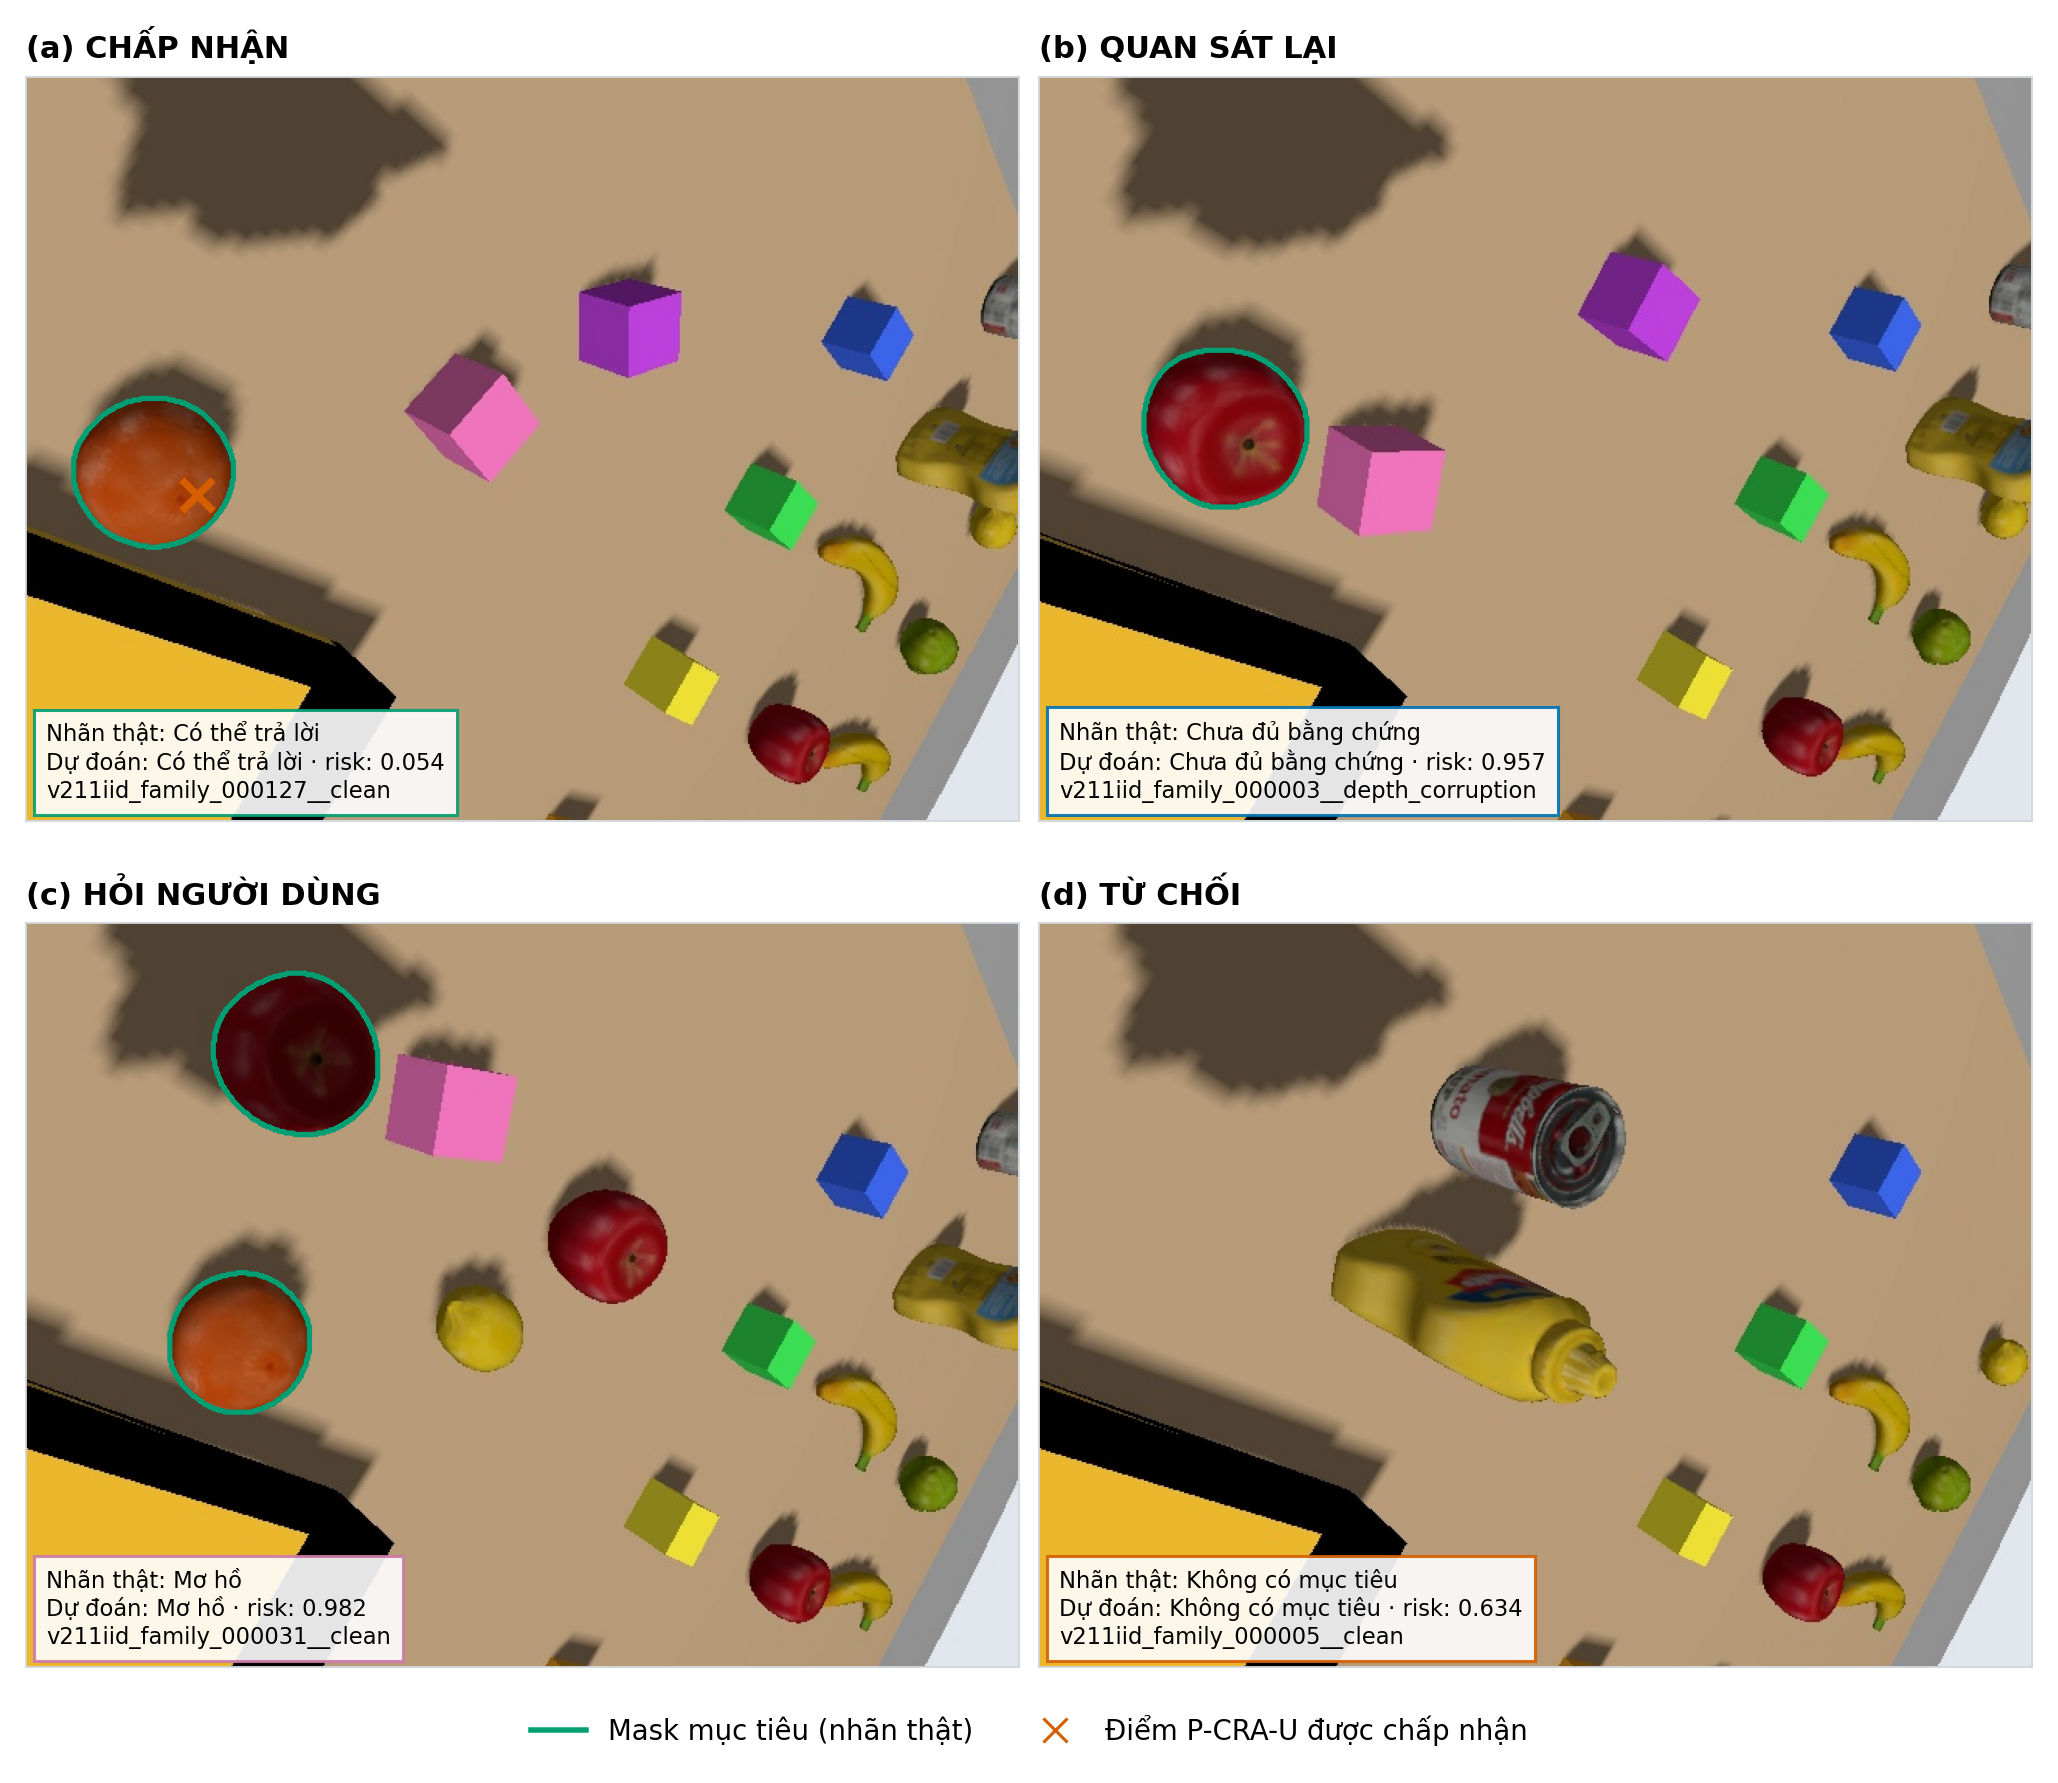
\includegraphics[width=\textwidth,height=0.72\textheight,keepaspectratio]{hinhanh/fig14_four_policy_decisions_adapter_vi.png}
    \caption{Bốn quyết định Adapter từ sample thật.
    Điểm cấp hành động chỉ thể hiện ở EXECUTE;
    các case còn lại chưa chứng minh recovery.}
    \label{fig:results-four-decisions}
    {\footnotesize Nguồn: RGB Gazebo, prediction, risk và runtime decision
    Adapter đã khóa.\par}
\end{figure}

\section{Kiểm chứng đường tích hợp Gazebo--UR3}
\label{sec:results-gazebo}

\subsection{Audit nhiều khung hình trước MoveIt}

Audit dưới đây dùng V2 lịch sử, chưa chạy lại bằng Adapter. Run audit dùng pose camera Test-IID nhưng trên
cảnh demo riêng, không phải năm sample test
mới. Năm frame có timestamp riêng được chạy
V2; prediction/decision được khóa trước khi
checker RGB-D và evaluator nhãn mô phỏng
đối chiếu vật đích.

Checker RGB-D không đọc semantic labels để
chọn vật trước inference. Nó kiểm tra một
thành phần đỏ đủ lớn, tương đối tròn và
depth phù hợp cho quả táo của cảnh cụ thể.
Đây là kiểm tra độc lập có phạm vi hẹp,
không phải object identity gate đã xác
nhận cho mọi vật thể.

\begin{table}[htbp]
    \centering
    \setlength{\tabcolsep}{4pt}
    \renewcommand{\arraystretch}{1.15}
    \caption{Audit năm frame tại pose camera Test-IID
    trong cảnh Gazebo demo riêng.}
    \label{tab:results-gazebo-frames}
    \small
    \begin{tabularx}{\textwidth}{@{}>{\raggedright\arraybackslash}Xrrrrl@{}}
        \toprule
        Frame & MAP $(u,v)$ & \shortstack{Depth tại\\điểm (m)} & Risk & \shortstack{Kiểm tra\\RGB-D} & Decision \\
        \midrule
        001 & $(150,210)$ & 0.45044 & 0.32664 & Đạt & ASK\_USER \\
        002 & $(150,210)$ & 0.44982 & 0.32682 & Đạt & ASK\_USER \\
        003 & $(150,210)$ & 0.44916 & 0.29459 & Đạt & ASK\_USER \\
        004 & $(150,210)$ & 0.44910 & 0.30674 & Đạt & ASK\_USER \\
        005 & $(150,210)$ & 0.44910 & 0.31965 & Đạt & ASK\_USER \\
        \bottomrule
    \end{tabularx}
    \vspace{2pt}
    {\footnotesize\raggedright Nguồn: \texttt{audit\_\allowbreak summary.json},
    run \texttt{iid\_\allowbreak pose\_\allowbreak audit\_\allowbreak 20261001T080100Z\_\allowbreak 49405}.
    Evaluator hậu kiểm xác nhận point-in-target và
    point-in-interior ở cả năm frame.\par}
\end{table}

Cả năm frame có điểm đúng và checker đạt,
nhưng decision đều ASK\_USER, nên pre-handoff
không đạt. Điểm đúng không đủ để tự ý thay
policy thành EXECUTE. Risk dao động khoảng
0.29459--0.32682, cao hơn threshold đã khóa;
không chỉnh threshold chỉ để demo chuyển động.

Maximum candidate jitter bằng 0 pixel
trên lưới dự đoán; mỗi ô tương ứng khoảng
$20\times20$ pixel ảnh. Sự ổn định này
chịu lượng tử hóa, không chứng minh không
có sai số subpixel hoặc 3D. Năm frame
cùng cảnh không phải năm trial độc lập
để ước lượng task success.

\begin{figure}[htbp]
    \centering
    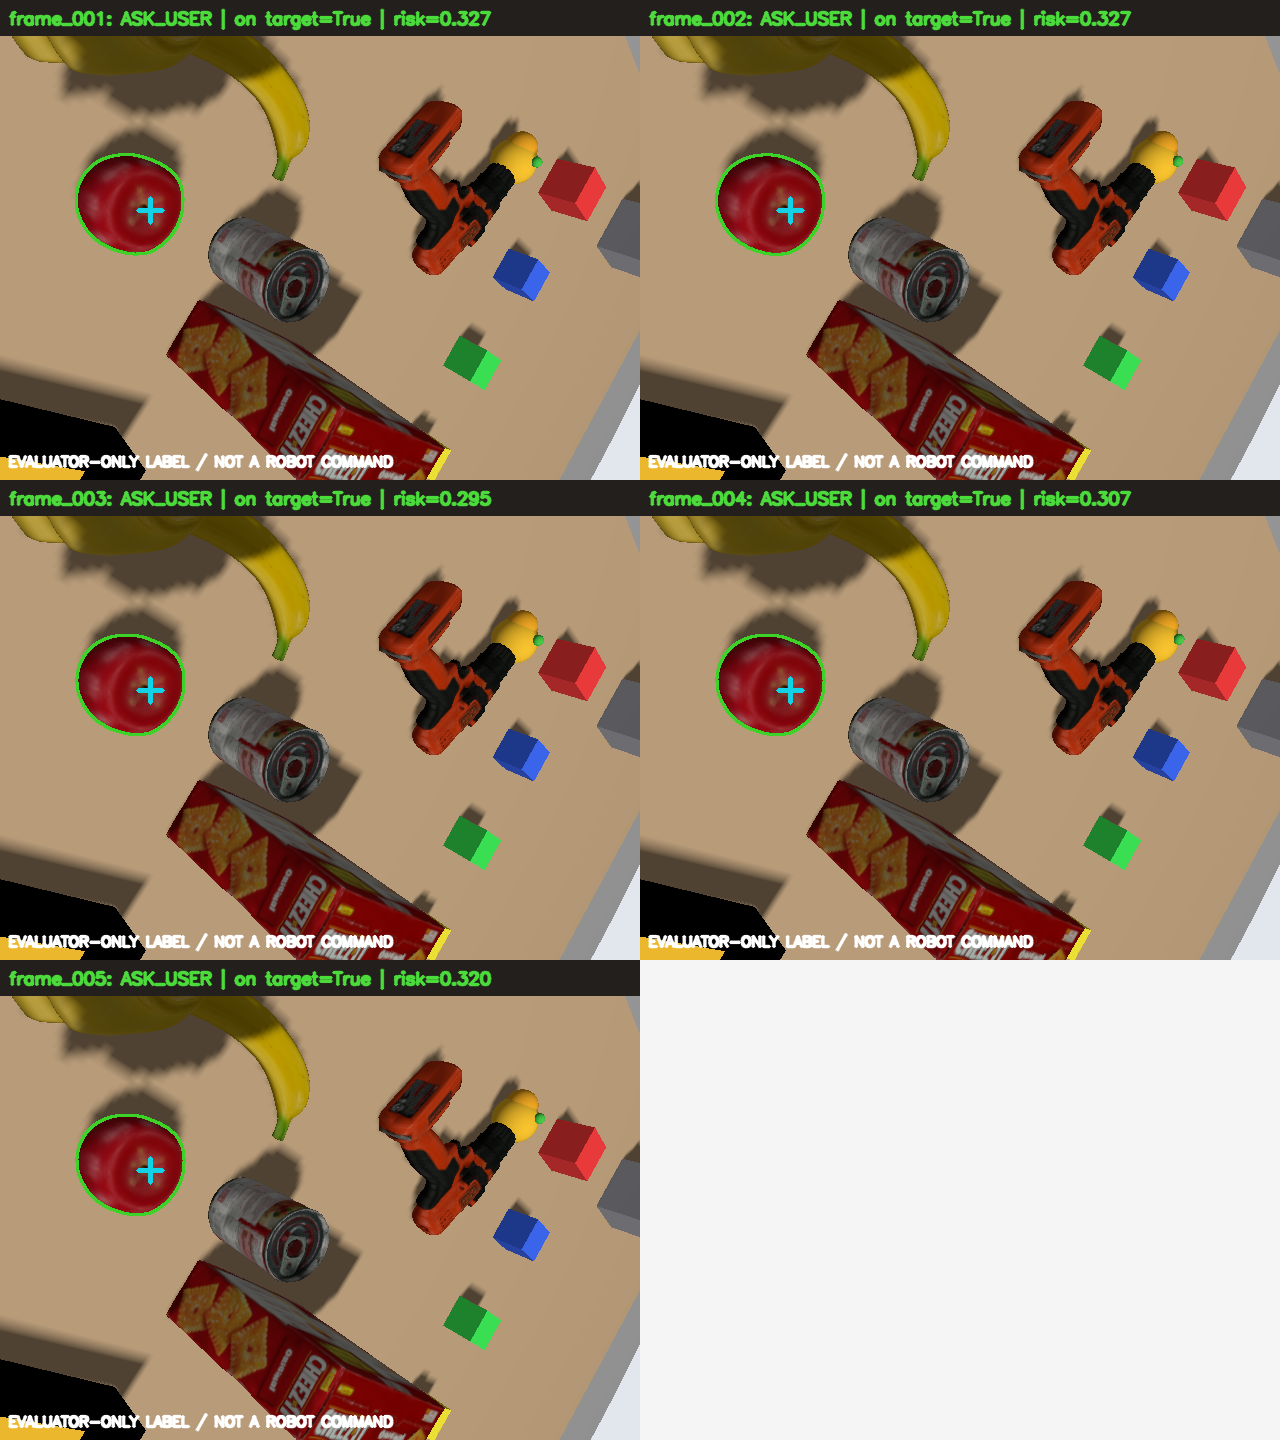
\includegraphics[width=\textwidth,height=0.72\textheight,keepaspectratio]{hinhanh/audit_montage.png}
    \caption{Audit năm frame: MAP ổn định và đúng
    target theo evaluator hậu kiểm, nhưng policy
    giữ ASK\_USER. Không có lệnh chuyển động robot.}
    \label{fig:results-gazebo-audit}
    {\footnotesize Nguồn: capture, prediction lock
    và montage của run audit Gazebo đã lưu.\par}
\end{figure}

\subsection{Kết quả nhận thức không phải kết quả thao tác}

\begin{table}[htbp]
    \centering
    \setlength{\tabcolsep}{4pt}
    \renewcommand{\arraystretch}{1.15}
    \caption{Ranh giới bằng chứng của demo downstream hiện tại.}
    \label{tab:results-downstream-status}
    \small
    \begin{tabularx}{\textwidth}{@{}>{\raggedright\arraybackslash}p{0.42\textwidth}r>{\raggedright\arraybackslash}X@{}}
        \toprule
        Nội dung kiểm tra & Kết quả & Phạm vi \\
        \midrule
        Điểm trong target / interior & 5/5 & Hậu kiểm trên năm frame \\
        Checker RGB-D không dùng nhãn & 5/5 & Checker quả táo riêng cho cảnh \\
        Metric depth consistency & 5/5 & Kiểm tra tại điểm ứng viên \\
        Pre-handoff đủ điều kiện & 0/5 & Cả năm decision ASK\_USER \\
        MoveIt nối với run audit & Không & Không truyền target từ V2 \\
        Robot motion được phát & Không & Không thực thi trajectory \\
        IK/planning success rate & -- & Chưa có trial tương ứng \\
        Grasp/lift/place success rate & -- & Chưa có trial tương ứng \\
        End-to-end task success & -- & Chưa đánh giá thao tác khép kín \\
        Wrong-object execution rate & -- & Chưa có lượt thực thi để chấm \\
        \bottomrule
    \end{tabularx}
    \vspace{2pt}
    {\footnotesize\raggedright Nguồn: audit summary và lock của run.
    Các metric thao tác chưa đo không được ghi 0\%
    hoặc suy từ 5/5 điểm đúng.\par}
\end{table}

Đánh giá robot còn cần chuyển điểm sang 3D
đúng CameraInfo/TF, kiểm tra workspace và
va chạm, chọn grasp pose, giải IK, điều
khiển gripper, xác minh lift/place và
ghi trial độc lập. Ba điều kiện forced
point, geometry gate và selective policy
chưa có thử nghiệm downstream công bằng.
World/URDF và log controller lịch sử
không thay cho bằng chứng V2 điều khiển.

Do đó, RQ5 được trả lời một phần bằng
giảm lỗi chấp nhận trên ảnh, chưa được
trả lời bằng tỉ lệ giảm sai vật trong
pick-and-place.

\begin{figure}[htbp]
    \centering
    \pcrauPendingResultsFigure{Chuỗi nhận target -- planning --
    grasp -- lift -- place, kèm log trial và xác minh trạng thái vật.}
    \caption{Kiểm chứng pick-and-place khép kín bằng
    best V2 (chưa có -- bổ sung sau).
    Cần thực hiện thí nghiệm thao tác; không chỉ
    thiếu ảnh minh họa.}
    \label{fig:results-robot-trial-pending}
    {\footnotesize Nguồn dự kiến: RGB/video Gazebo,
    MoveIt/controller log và evaluator trial độc lập.\par}
\end{figure}

\section{Phân tích các trường hợp điển hình}
\label{sec:results-case-study}

\subsection{Các case từ prediction thật}

Các case được chọn để giải thích hành vi, không
để ước lượng accuracy tổng. ID viết ngắn trong
Bảng~\ref{tab:results-case-study} có tiền tố
\texttt{v211iid\_\allowbreak family\_\allowbreak }; ký hiệu CF là
counterfactual. Tất cả risk, MAP và decision
đều lấy từ output đã lưu, không sửa theo nhãn.

\begin{table}[htbp]
    \centering
    \setlength{\tabcolsep}{4pt}
    \renewcommand{\arraystretch}{1.15}
    \caption{Case study từ Test-IID.
    Hit chỉ có nghĩa point-in-target, không phải task success.}
    \label{tab:results-case-study}
    \small
    \begin{tabularx}{\textwidth}{@{}>{\raggedright\arraybackslash}p{0.23\textwidth}>{\raggedright\arraybackslash}Xrrl@{}}
        \toprule
        Family / variant & \shortstack{Nhãn thật\\$\rightarrow$ dự đoán} & MAP & Risk & Decision \\
        \midrule
        000127 / clean & FOUND $\rightarrow$ FOUND &
        $(110,270)$ & 0.05371 & EXECUTE \\
        000031 / clean & AMBIG. $\rightarrow$ AMBIG. &
        $(130,290)$ & 0.98228 & ASK\_USER \\
        000003 / depth & INSUFF. $\rightarrow$ INSUFF. &
        $(130,250)$ & 0.95749 & REOBSERVE \\
        000005 / clean & ABSENT $\rightarrow$ ABSENT &
        $(270,250)$ & 0.63358 & ABSTAIN \\
        000127 / semantic CF & FOUND $\rightarrow$ FOUND &
        $(270,230)$ & 0.02632 & EXECUTE \\
        000002 / clean & FOUND $\rightarrow$ FOUND &
        $(170,290)$ & 0.04316 & EXECUTE \\
        000165 / relation CF & FOUND $\rightarrow$ INSUFF. &
        $(290,170)$ & 0.70824 & REOBSERVE \\
        \bottomrule
    \end{tabularx}
    \vspace{2pt}
    {\footnotesize\raggedright Nguồn: prediction và decision Test-IID.
    Ba hàng đầu và semantic CF hit target; hai
    hàng cuối không hit. ABSENT không có target mask,
    nên điểm của hàng này không có grounding score hợp lệ.\par}
\end{table}

\subsection{Target rõ và câu lệnh mơ hồ}

Family 127 clean có risk 0.05371, thấp hơn
threshold Adapter 0.26119, nhãn/dự đoán FOUND và MAP
trong target. Policy cho EXECUTE. Hình
heatmap ở Mục~\ref{sec:results-grounding}
minh họa một trường hợp nhận thức phù hợp;
chưa có grasp trial gắn với sample này.

Family 031 clean có nhiều vùng xác suất,
answerability AMBIGUOUS và spatial score
0.99830. MAP vẫn nằm trong target mask hợp
nhưng risk 0.98228 và decision ASK\_USER.
Case này cho thấy một điểm đúng không đủ
để thực hiện câu lệnh chưa phân giải.

\subsection{Depth hỏng và target absent}

Family 003 depth corruption có source
depth 0.96211, nhãn/dự đoán INSUFFICIENT,
risk 0.95749 và REOBSERVE. MAP trong mask
không phủ nhận việc bằng chứng depth
không đủ. Đây là perturbation relative
depth, không phải một thử nghiệm missing
depth toàn ảnh nếu manifest không ghi vậy.

Family 005 clean có nhãn/dự đoán ABSENT,
risk 0.63358 và ABSTAIN. Điểm ứng viên
$(270,250)$ vẫn có thể được head xuất,
nhưng không có target hợp lệ để cấp
cho hành động. Không chấm một pixel bất
kỳ như grounding đúng của absent.

\subsection{False positive source và hồi quy grounding}

Family 127 semantic CF vẫn FOUND và
MAP đúng, risk chỉ 0.02632. Tuy nhiên,
semantic score 0.65666 vượt threshold
0.5 trong khi nhãn semantic bằng 0.
Case này minh họa phản ứng với thay
đổi câu lệnh nhưng attribution thừa.
Không dùng tên variant để thay nhãn
source thực rồi gọi dự đoán này đúng.

Family 002 clean có RoboRefer đúng nhưng MAP sidecar sai.
V2 lịch sử đoán INSUFFICIENT, risk 0.50223 và REOBSERVE; Adapter đổi
sang FOUND, risk 0.04316 và EXECUTE dù điểm vẫn sai. Đây là hồi quy
quyết định đáng chú ý: tăng tự tin không tự sửa được lỗi định vị.
Occlusion score 0.53704 vẫn là false positive theo nhãn đã lưu;
chưa quy lỗi nhân quả cho source này.

Family 165 relation CF là ví dụ cả
hai mô hình sai. Adapter có risk 0.70824
và REOBSERVE, nên không cấp điểm
sai cho execute. Source occlusion
0.69925 trong khi nhãn source bằng
0 cho thấy một failure có thể được
chặn nhưng lý do attribution chưa
đúng theo supervision.

\begin{figure}[htbp]
    \centering
    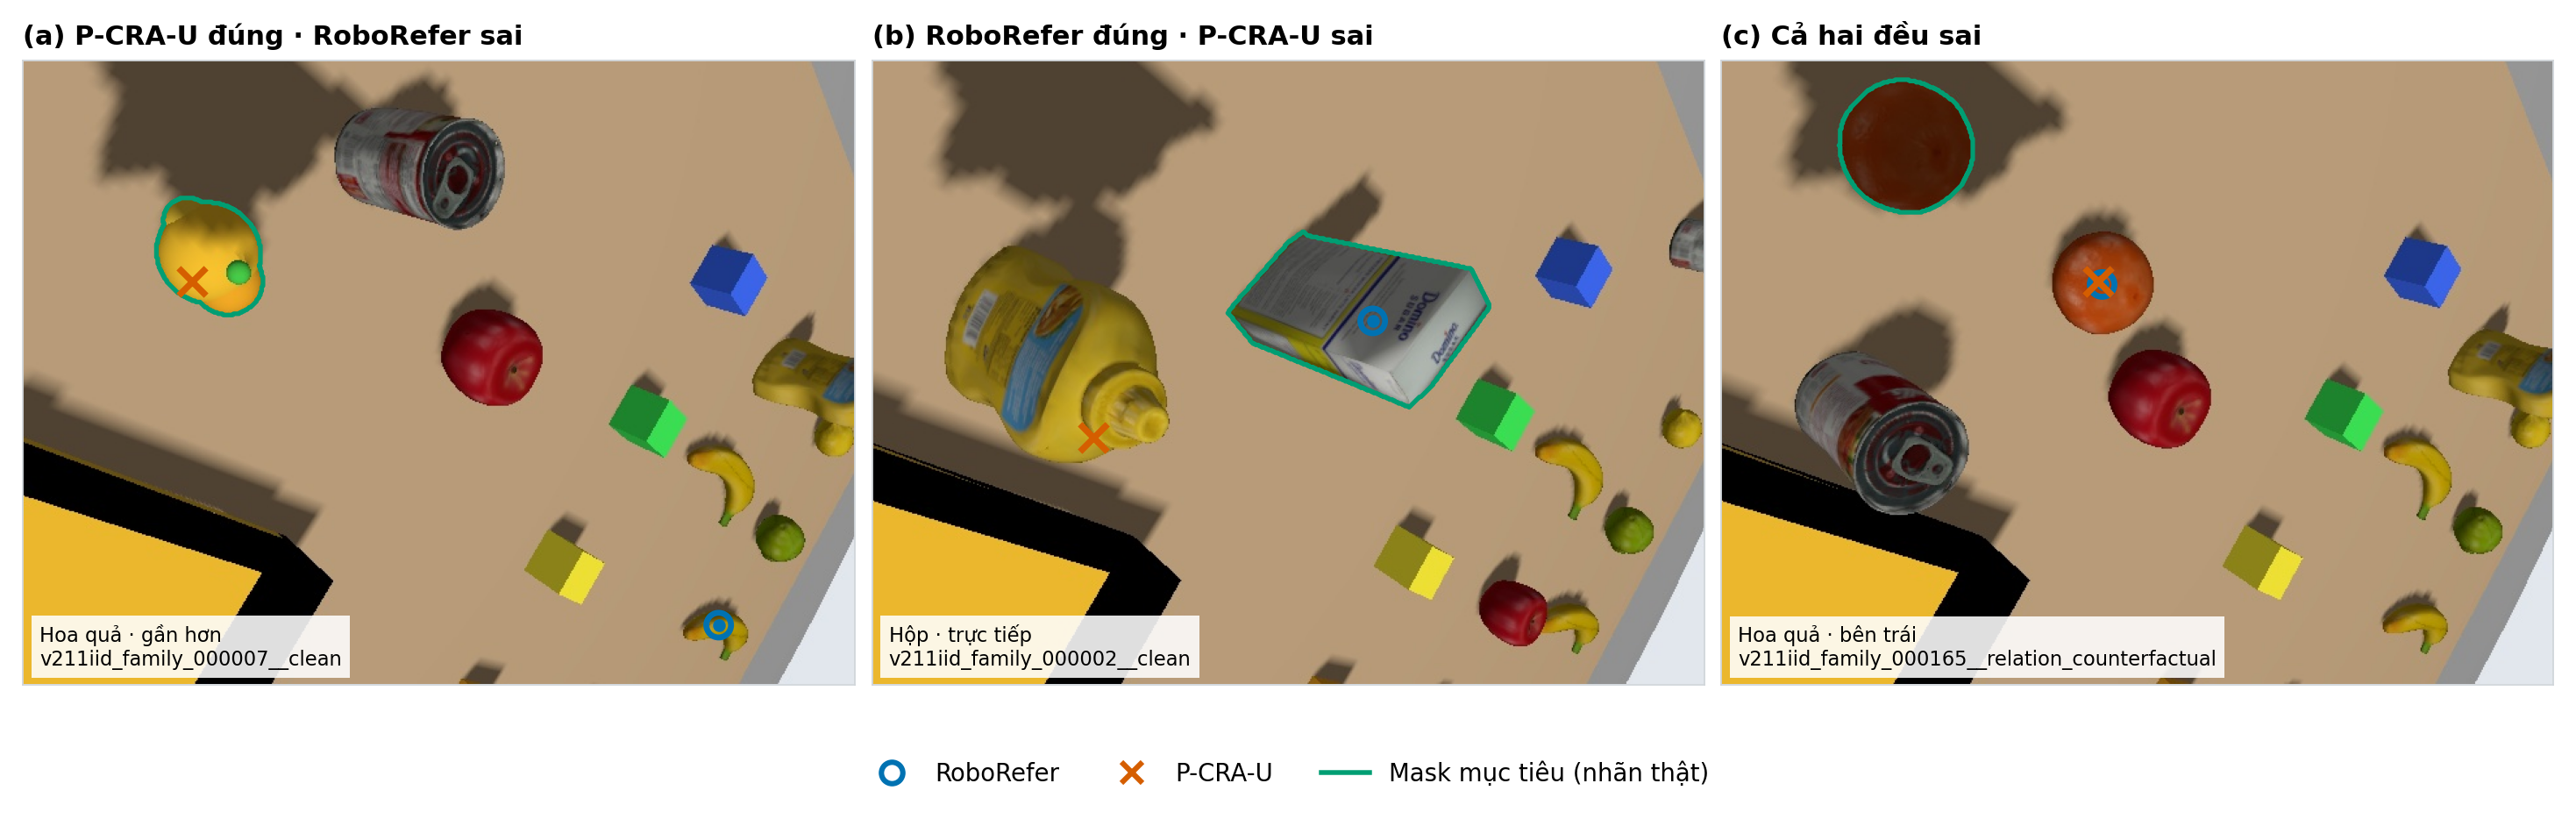
\includegraphics[width=\textwidth,height=0.68\textheight,keepaspectratio]{hinhanh/fig15_paired_success_and_failure_adapter_vi.png}
    \caption{Ba case paired: V2 đúng--RoboRefer sai
    (000007 clean), RoboRefer đúng--V2 sai
    (000002 clean) và cả hai sai
    (000165 relation counterfactual).
    Hình minh họa, không thay số liệu toàn tập.}
    \label{fig:results-paired-failure-cases}
    {\footnotesize Nguồn: RGB Gazebo, điểm của hai
    mô hình và mask evaluator Test-IID đã lưu.\par}
\end{figure}

Case occluded anchor cần có anchor prediction
và annotation visibility riêng để phân tích
đúng nguyên nhân. Hình source hiện có là
occlusion/view counterfactual, chưa đủ để
khẳng định đúng một anchor bị che là nguyên
nhân duy nhất của quyết định.

\section{Phân tích lỗi và thảo luận}
\label{sec:results-failure-analysis}

\subsection{Phân tách lỗi theo tầng}

Grounding, answerability, source attribution,
calibration và controller có event khác nhau.
Một điểm đúng nhưng nhãn AMBIGUOUS không
phải failure localization; một controller
timeout không tự là failure perception.
Bảng~\ref{tab:results-failure-layers} tổng
hợp bằng chứng và phần chưa thể quy nguyên nhân.

\begin{table}[htbp]
    \centering
    \setlength{\tabcolsep}{4pt}
    \renewcommand{\arraystretch}{1.15}
    \caption{Failure analysis theo tầng và giới hạn quy nguyên nhân.}
    \label{tab:results-failure-layers}
    \small
    \begin{tabularx}{\textwidth}{@{}>{\raggedright\arraybackslash}p{0.18\textwidth}>{\raggedright\arraybackslash}p{0.35\textwidth}>{\raggedright\arraybackslash}X@{}}
        \toprule
        Tầng & Bằng chứng hiện có & Diễn giải/giới hạn \\
        \midrule
        Ngôn ngữ & Chưa có parser exact-match riêng &
        Không quy mọi lỗi relation cho parser \\
        Grounding & 60/835 điểm sai; 56 RoboRefer-only &
        Hồi quy tập trung đáng kể ở box; cần kiểm tra có kiểm soát \\
        Relation & 145/650 cạnh proxy sai &
        Không tương đương 145 mệnh đề hình học sai \\
        Spatial region & 110/835 không đạt score coverage &
        Empirical thấp hơn nominal; cần giữ event rời rạc \\
        Answerability & 189/1000 phân loại sai; 55 false FOUND &
        Nhầm ABSENT--INSUFFICIENT ảnh hưởng loại can thiệp \\
        Source & Semantic FP 272; occlusion FP 141 &
        Cảnh báo thừa, chưa là attribution nhân quả \\
        Risk/policy & 34/361 execute có lỗi nhận thức &
        Lỗi chấp nhận chưa bằng wrong-object execution thật \\
        Robot & Chưa có trial khép kín &
        Không gộp MoveIt/controller failure vào metric nhận thức \\
        \bottomrule
    \end{tabularx}
    \vspace{2pt}
    {\footnotesize\raggedright Nguồn: grounding, edge, source,
    answerability/policy Adapter và audit V2 lịch sử.\par}
\end{table}

\subsection{Mức cải thiện và ý nghĩa đối với khoảng trống nghiên cứu}

\paragraph{Định vị và điều kiện chấp nhận là hai mục tiêu riêng.}
P-CRA-U cải thiện grounding target-present so với RoboRefer, với paired
CI không chứa 0. Tuy nhiên, nguồn tăng chính ở AMBIGUOUS cho thấy kết quả
này chủ yếu mở rộng khả năng định vị tới tập ứng viên, chưa đồng nghĩa
chọn được một referent duy nhất. FOUND-only chưa có CI chênh lệch loại
trừ 0, còn hộp hồi quy mạnh. Việc báo đồng thời grounding và answerability
làm rõ giới hạn của accuracy điểm đơn lẻ, đúng với khoảng trống đặt ở
Chương~1--2.

\paragraph{Evidence phong phú chưa tự tạo ra độ tin cậy.}
Spatial distribution, anchor/edge và source đã có đường dự đoán, nhưng
khả năng phát hiện lỗi cần được đo riêng. Phân tích trên FOUND cho thấy
entropy và margin liên hệ yếu với sai lệch vị trí; source depth phản ứng
tốt hơn các source không yếu khác, trong khi semantic/occlusion còn nhiều
cảnh báo thừa. Kết quả này chỉ ra nhu cầu kiểm chứng evidence bằng metric,
thay vì diễn giải heatmap sắc hoặc score nguồn cao như một giải thích đúng.

\paragraph{Hiệu chuẩn tạo cải thiện xác suất trong phạm vi so sánh.}
Logistic33 có Brier/NLL/ECE tốt hơn raw score Adapter, nhưng AUROC/AP và AURC kém hơn raw. So với logistic18 V2, các metric này tốt hơn; hai phép đối chiếu cần được tách rõ. Vùng không gian đã được đánh giá bằng cả score coverage, direct
intersection và coverage--area. Hai event coverage khác nhau cho thấy
quy tắc rời rạc là một phần của định nghĩa phép đo. Các kết quả củng cố
quy trình hiệu chuẩn và đánh giá đầu ra; chưa cô lập lợi ích riêng của
source conditioning hoặc xác lập bảo đảm conformal theo family.

\paragraph{Giá trị của hệ thống được kiểm chứng ở mức nhận thức.}
Policy Adapter nhận thêm 78 ca hợp lệ nhưng selective risk tăng lên 9.42\%, vượt ngân sách calibration 7.5\%,
và audit xác nhận đường Gazebo--RGB-D--prediction--decision. Đây là phần
đã làm được của ý tưởng nối grounding với quyết định sử dụng kết quả.
REOBSERVE/ASK\_USER chưa có đánh giá recovery, audit chưa handoff MoveIt,
nên kết luận chưa mở rộng đến giảm sai vật hay tăng thành công gắp--đặt.

Như vậy, tính đóng góp của đồ án nằm ở thiết kế tích hợp có thể truy
nguyên và các phép kiểm chứng tương ứng trên Test-IID. Khoảng trống đã
được xử lý một phần bằng đầu ra đa nhiệm và risk; phần còn lại là đối
chứng cô lập, chất lượng graph/instance và hiệu quả downstream. Việc
phân biệt các mức này giữ cho ý tưởng thiết kế, cải thiện thực nghiệm và
tính mới tuyệt đối không bị đồng nhất.

\subsection{Nguy cơ ảnh hưởng độ tin cậy}

\paragraph{Phụ thuộc dữ liệu.}
Năm variant cùng family không độc lập.
CI grounding đã dùng cluster bootstrap,
và CI Adapter đã có cho macro-F1, coverage, selective risk cùng valid recall; chưa có CI cùng đơn vị cho mọi source hoặc calibration metric.
Các phân tầng nhỏ có CI rộng và chưa
hiệu chỉnh multiple comparisons.

\paragraph{Giới hạn miền mô phỏng.}
Registry, texture, mẫu câu và cơ chế
perturbation hữu hạn. Relative depth
corruption dùng phép tổng hợp như dịch
vòng, không mô phỏng đầy đủ nhiễu cảm
biến. Không suy rộng sang robot vật lý,
asset mới hoặc miền OOD chưa đo.

\paragraph{Giới hạn supervision.}
Spatial source là nhãn yếu; relation
edge là proxy. Mask hợp cho AMBIGUOUS
làm hit có nghĩa khác với instance
identification. Chưa có oracle graph
hay evaluator anchor toàn diện.

\paragraph{Thiếu ablation và biến thiên seed.}
V2 chính là một seed. Ba seed V3 có
nhiều thay đổi đồng thời và không
đạt cổng, không thay bằng chứng nhiều
seed cho V2. Không tách được đóng góp
của từng head/loss khi thiếu retrain
ablation và calibrator tương ứng.

\paragraph{Khác phạm vi tính toán.}
V2 test dùng cache tower, RoboRefer
gốc sinh token. Không so cache-only
sidecar latency với inference gốc
rồi gọi là tốc độ end-to-end.
Chi phí tower, tiền xử lý, I/O và
camera phải được tính cùng phạm vi.

\paragraph{Bộ test đã được quan sát.}
Artifact V2 ban đầu được giữ nguyên. Phân tích lỗi của IID cũ đã
tham gia định hướng vòng phát triển Adapter; dù gradient chỉ dùng
train và lựa chọn mô hình/ngưỡng không fit bằng test, đánh giá lại
trên bộ đã xem không tương đương xác nhận mới độc lập. Các CI mô tả
biến thiên cluster trên bộ này, không loại bỏ ảnh hưởng của lựa chọn
nghiên cứu qua nhiều vòng. Nếu phát triển tiếp từ các lỗi đã thấy,
cần một bộ IID mới để xác nhận trước khi khái quát kết luận.

\subsection{Tổng hợp câu trả lời cho RQ1--RQ5}

\begin{table}[htbp]
    \centering
    \setlength{\tabcolsep}{4pt}
    \renewcommand{\arraystretch}{1.15}
    \caption{Tổng hợp bằng chứng theo câu hỏi nghiên cứu.}
    \label{tab:results-rq-summary}
    \small
    \begin{tabularx}{\textwidth}{@{}l>{\raggedright\arraybackslash}p{0.47\textwidth}>{\raggedright\arraybackslash}X@{}}
        \toprule
        Câu hỏi & Bằng chứng định lượng & Kết luận trong phạm vi đo \\
        \midrule
        RQ1 & PIT $+6.11$ pp, CI $[1.78,10.49]$;
        FOUND-only $+1.90$ pp, CI chứa 0 &
        Có cải thiện toàn hệ thống target-present,
        chưa cô lập relation và không đều theo nhóm \\
        RQ2 & Answer macro-F1 0.8097;
        false FOUND 55/580 non-FOUND &
        Head hữu ích nhưng chưa loại hết chấp nhận sai;
        localization ranking riêng còn thiếu \\
        RQ3 & Depth $\Delta u=+0.4304$;
        semantic FP 272, occlusion FP 141 &
        Có phản ứng theo perturbation,
        attribution còn hạn chế \\
        RQ4 & Brier raw/fit 0.08014/0.07711;
        ECE 0.04847/0.03108;
        region score/direct 86.83\%/95.81\% &
        Brier/ECE tốt hơn raw, ranking kém hơn raw; hai event vùng
        được tách; thiếu scalar-only/source ablation \\
        RQ5 & Valid recall 80.74\%, error 9.42\%
        ở coverage 36.10\%;
        audit chưa handoff, chưa robot motion &
        Có bằng chứng chọn lọc trong nhận thức,
        chưa kết luận hiệu quả thao tác \\
        \bottomrule
    \end{tabularx}
    \vspace{2pt}
    {\footnotesize\raggedright Nguồn: tổng hợp các bảng và
    artifact đã phân tích trong chương; không bổ
    sung kết quả của thí nghiệm chưa chạy.\par}
\end{table}

P-CRA-U có Adapter giữ cải thiện grounding của V2 và cải thiện
answerability cùng số ca hợp lệ được nhận. Mức tăng coverage đổi lấy
nhiều lỗi chấp nhận hơn, đặc biệt ở che khuất và quan hệ; chưa đạt
ngân sách lỗi 7.5\% trên IID cũ. Hồi quy nhóm hộp, false positive source,
score coverage dưới nominal và thiếu ablation/robot motion vẫn còn.
Các kết quả mới không thay đổi trạng thái của bằng chứng chưa đo.

Chương~6 sẽ tổng kết đóng góp trong đúng
phạm vi này và nêu hướng hoàn thiện,
không biến phần chưa đo thành kết quả.
